% **************************************************
% Document Class Definition
% **************************************************
\documentclass[%
	paper=A4,					% paper size --> A4 is default in Germany
	twoside=true,				% onesite or twoside printing
	openright,					% doublepage cleaning ends up right side
	parskip=full,				% spacing value / method for paragraphs
	chapterprefix=true,			% prefix for chapter marks
	11pt,						% font size
	headings=normal,			% size of headings
	bibliography=totoc,			% include bib in toc
	listof=totoc,				% include listof entries in toc
	titlepage=on,				% own page for each title page
	captions=tableabove,		% display table captions above the float env
	draft=true, 				% value for draft version
]{scrreprt}%

% **************************************************
% Debug LaTeX Information
% **************************************************
%\listfiles

% **************************************************
% Information and Commands for Reuse
% **************************************************
\newcommand{\thesisTitle}{
	Mixed Reality Media: Integration of live video feed in 3D environments
}
\newcommand{\thesisName}{Martin Zier}
\newcommand{\thesisSubject}{Bachelor Thesis}
\newcommand{\thesisDate}{\today}
\newcommand{\thesisVersion}{Initial Drafting}

\newcommand{\thesisFirstReviewer}{Kristian Hildebrand}
\newcommand{\thesisFirstReviewerUniversity}{\protect{Beuth University of Applied Sciences}}
\newcommand{\thesisFirstReviewerDepartment}{Department VI: Computer Sciences and Media}

\newcommand{\thesisSecondReviewer}{Prof. Dr.-Ing. Ren\'e G\"orlich}
\newcommand{\thesisSecondReviewerUniversity}{\protect{Beuth University of Applied Sciences}}
\newcommand{\thesisSecondReviewerDepartment}{Department VI: Computer Sciences and Media}

\newcommand{\thesisFirstSupervisor}{Kristian Hildebrand}
\newcommand{\thesisSecondSupervisor}{Joachim Quantz}

\newcommand{\thesisUniversity}{\protect{Beuth University of Applied Sciences}}
\newcommand{\thesisUniversityDepartment}{Department VI: Computer Sciences and Media}
\newcommand{\thesisUniversityInstitute}{ }
\newcommand{\thesisUniversityGroup}{ }
\newcommand{\thesisUniversityCity}{Berlin}
\newcommand{\thesisUniversityStreetAddress}{Luxemburger Stra{\ss}e 10}
\newcommand{\thesisUniversityPostalCode}{13353}

% **************************************************
% Load and Configure Packages
% **************************************************
\usepackage[utf8]{inputenc}		% defines file's character encoding
\usepackage[english]{babel} % babel system, adjust the language of the content
\usepackage[					% clean thesis style
	figuresep=colon,%
	sansserif=false,%
	hangfigurecaption=false,%
	hangsection=true,%
	hangsubsection=true,%
	colorize=full,%
	colortheme=bluemagenta,%
	bibsys=bibtex,%
	bibfile=bib-refs,%
	bibstyle=alphabetic,%
]{cleanthesis}

\usepackage{todonotes}		% orange big fat todo notes inside the pdf
\usepackage{listings}		% code listings
\usepackage{amsmath}		% huh.
\usepackage{mathtools}		% uhh?
\usepackage{subcaption}		% allows for multiple figures in one big figure
\usepackage{cleveref}		% allow for appendix references
\usepackage[toc]{appendix}	% generate appendix
\reversemarginpar
\setlength{\marginparwidth}{3.5cm}
\hypersetup{					% setup the hyperref-package options
	pdftitle={\thesisTitle},	% 	- title (PDF meta)
	pdfsubject={\thesisSubject},% 	- subject (PDF meta)
	pdfauthor={\thesisName},	% 	- author (PDF meta)
	plainpages=false,			% 	-
	colorlinks=false,			% 	- colorize links?
	pdfborder={0 0 0},			% 	-
	breaklinks=true,			% 	- allow line break inside links
	bookmarksnumbered=true,		%
	bookmarksopen=true			%
}

% Glossaries needs to be after hyperref to enable linking.
\usepackage[toc]{glossaries} 

\makeglossaries
% !TeX spellcheck = en_US
% !TEX root = ../thesis-example.tex
%

\begingroup
\let\cleardoublepage\clearpage

\chapter{Unitys' Monobehaviour Loop}
\label{app:engineloop}

The behavior of a Unity-initiated object is outlined by the following 
flowchart in \ref{fig:appendix:monoflow}, taken from Unitys' manual.

\begin{figure}[htb]
	\centering
	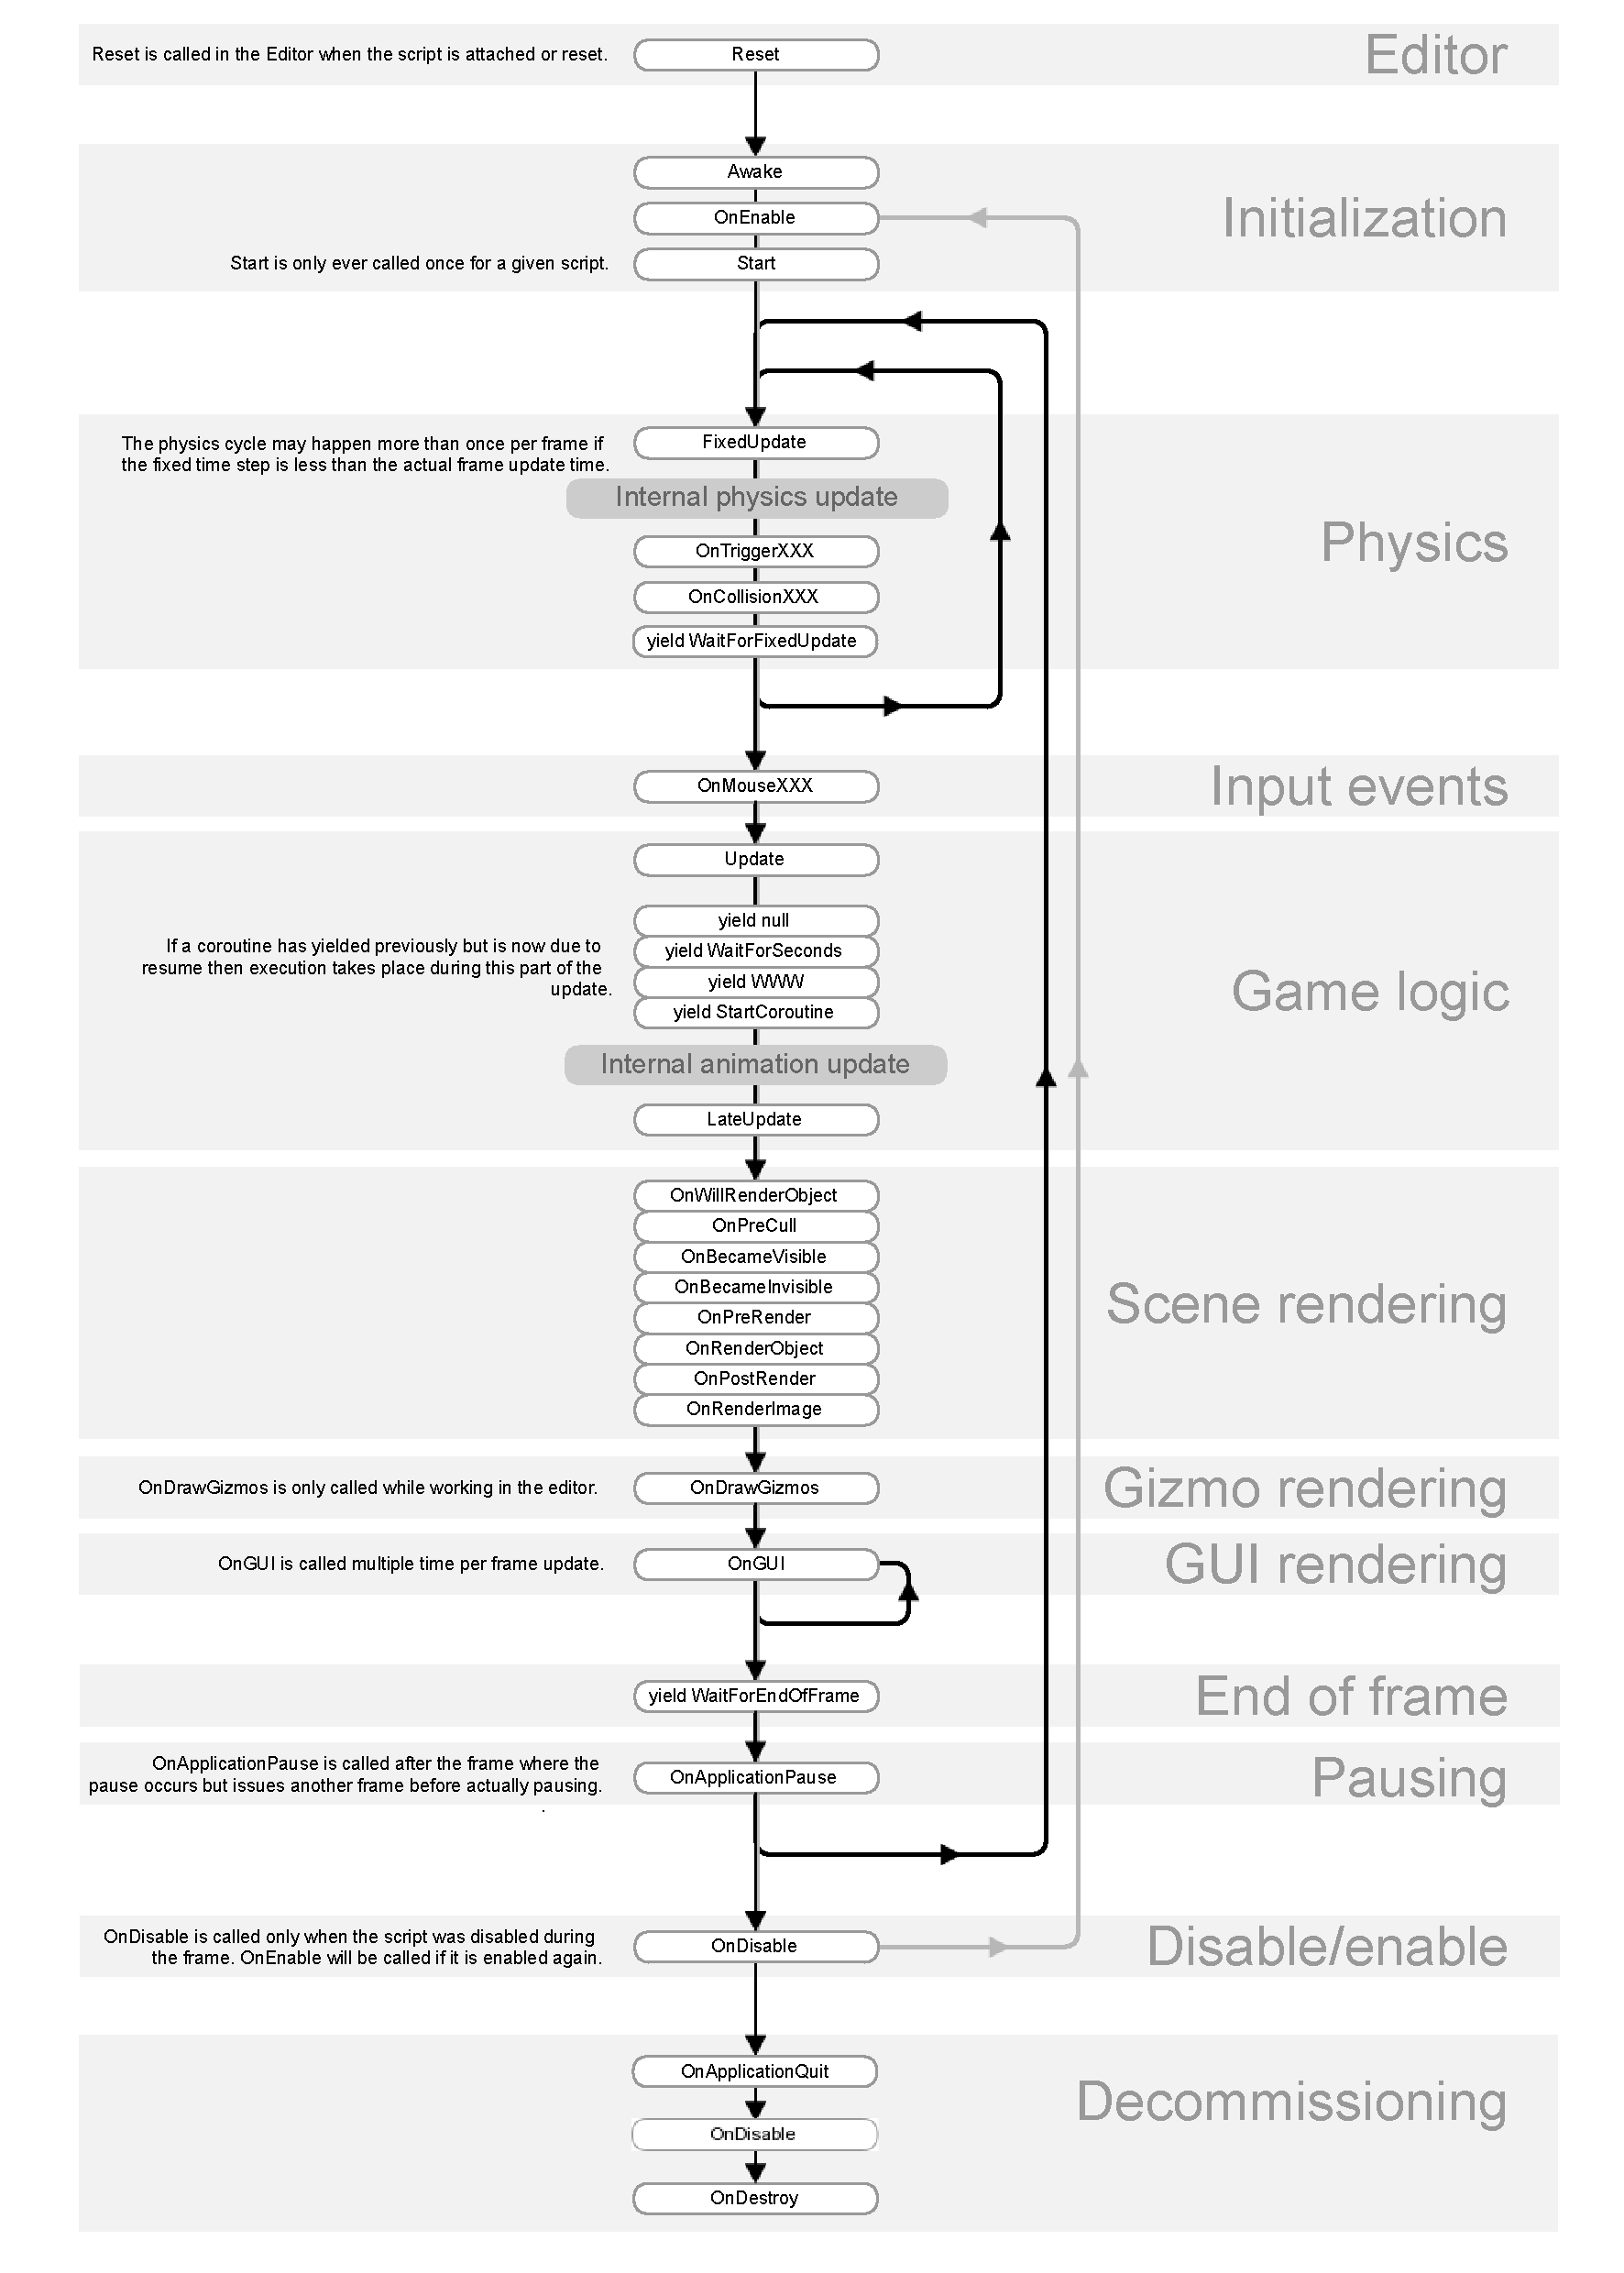
\includegraphics[width=0.85\textwidth]{_external/media/monobehaviour_flowchart2.pdf}
	\caption{Monobehaviour Flowchart}
	\label{fig:appendix:monoflow}
\end{figure}


\chapter{Simple Green Screen Setup}

Building a green screen set is no easy task and takes a lot of careful 
consideration in light setup, background coloring and material used on set. 
\newline
Figure \ref{fig:appendix:gs-setup} shows a very simple and low-cost green 
screen setup after Foster et al. \cite{foster:greenscreen:2010}

\begin{figure}[htb]
	\centering
	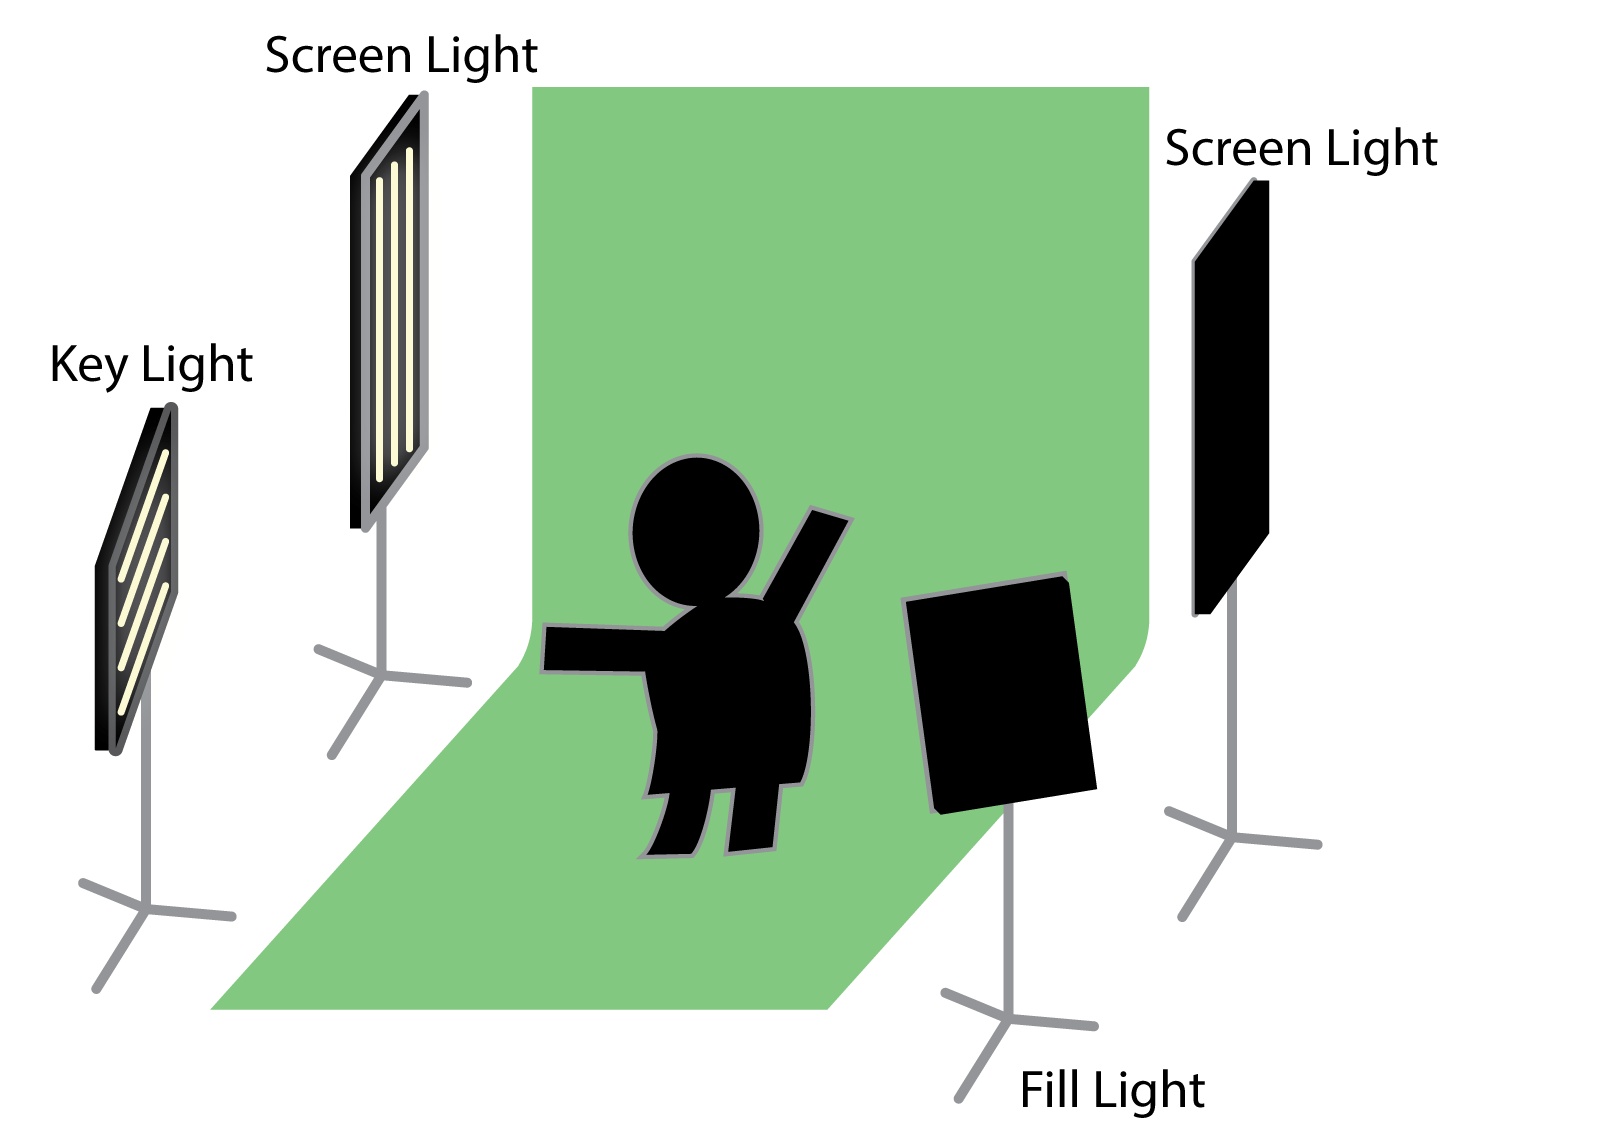
\includegraphics[width=\textwidth]{gfx/appendix/gs-setup.png}
	\caption{Basic green screen setup}
	\label{fig:appendix:gs-setup}
\end{figure}

\endgroup % actually is a glossary, sorry.

% **************************************************
% Document CONTENT
% **************************************************
\begin{document}

% --------------------------
% rename document parts
% --------------------------
%\renewcaptionname{ngerman}{\figurename}{Abb.}
%\renewcaptionname{ngerman}{\tablename}{Tab.}
\renewcaptionname{english}{\figurename}{Fig.}
\renewcaptionname{english}{\tablename}{Tab.}

% --------------------------
% Front matter
% --------------------------
\pagenumbering{roman}			% roman page numbing (invisible for empty page style)
\pagestyle{empty}				% no header or footers
% !TEX root = ../thesis-example.tex
% ------------------------------------  --> main title page
\begin{titlepage}
	\pdfbookmark[0]{Titlepage}{Titlepage}
	\tgherosfont
	\centering

	
\includegraphics[width=12cm]{_external/media/Beuth-Logo.png} \\[2mm]
	\textsf{\thesisUniversityDepartment} \\
	\textsf{\thesisUniversityInstitute} \\
	\textsf{\thesisUniversityGroup} \\

	\vfill
	{\large \thesisSubject} \\[5mm]
	{\LARGE \color{ctcolortitle}\textbf{\thesisTitle} \\[10mm]}
	{\Large \thesisName} \\

	\vfill
	\begin{minipage}[t]{.27\textwidth}
		\raggedleft
		\textit{1. Reviewer}
	\end{minipage}
	\hspace*{15pt}
	\begin{minipage}[t]{.65\textwidth}
		{\Large \thesisFirstReviewer} \\
	  	{\small \thesisFirstReviewerDepartment} \\[-1mm]
		{\small \thesisFirstReviewerUniversity}
	\end{minipage} \\[5mm]
	\begin{minipage}[t]{.27\textwidth}
		\raggedleft
		\textit{2. Reviewer}
	\end{minipage}
	\hspace*{15pt}
	\begin{minipage}[t]{.65\textwidth}
		{\Large \thesisSecondReviewer} \\
	  	{\small \thesisSecondReviewerDepartment} \\[-1mm]
		{\small \thesisSecondReviewerUniversity}
	\end{minipage} \\[10mm]
	\begin{minipage}[t]{.27\textwidth}
		\raggedleft
		\textit{Supervisor}
	\end{minipage}
	\hspace*{15pt}
	\begin{minipage}[t]{.65\textwidth}
		\thesisFirstSupervisor\
	\end{minipage} \\[10mm]

	\thesisDate \\

\end{titlepage}


% ------------------------------------  --> lower title back for single page layout
\hfill
\vfill
{
	\small
	\textbf{\thesisName} \\
	\textit{\thesisTitle} \\
	\thesisSubject, \thesisDate \\
	Reviewers: \thesisFirstReviewer\ and \thesisSecondReviewer \\
	Supervisor: \thesisFirstSupervisor \\[1.5em]
	\textbf{\thesisUniversity} \\
%	\textit{\thesisUniversityGroup} \\
%	\thesisUniversityInstitute \\
	\thesisUniversityDepartment \\
	\thesisUniversityStreetAddress \\
	\thesisUniversityPostalCode\ \thesisUniversityCity
}
		% INCLUDE: all titlepages
\cleardoublepage

\pagestyle{plain}				% display just page numbers
% !TeX spellcheck = en_US
% !TEX root = ../thesis-example.tex
%
\pdfbookmark[0]{Abstract}{Abstract}
\chapter*{Abstract}
\label{sec:abstract}
\vspace*{-10mm}

Virtual Reality is no distance dream anymore, but the technology has a 
marketing problem: A view through the eyes of the head-mounted display wearer 
is bland and loses the usage context. Following the first-person view is hard 
and it shows twitchy, unnatural motion.

This thesis discusses a general rendering pipeline for runtime 3D engines for 
Mixed Reality Media, a form of video composition that places a real person 
inside a virtual reality scene. The real world video will be augmented by 
multiple video techniques and parameters from the virtual environment.
\newline
For example this allows for recreation of light conditions from the virtual 
scene and creates an immersive and inviting view into the virtual scenery.

\begin{center}
	\hrulefill
\end{center}

VR ist kein entfernter Traum mehr, doch die Technologie hat ein 
Marketing-Problem: Ein Blick durch die Augen des Headset-Trägers ist 
uninteressant und verliert den Nutzerkontext. Der First-Person Sicht ist nur 
schwer zu folgen und zeigt unruhige, unnatürliche Bewegungen.

Diese Bachelor Arbeit beschäftigt sich mit dem Aufbau einer allgemeinen Mixed 
Reality Pipeline für Echtzeit 3D Engines, eine Aufarbeitung von 
Echtbildaufnahmen eines VR Nutzers und die Rückführung in eine virtuelle Szene. 
Durch mehrere Videoverfahren wird das Bild des Trägers mit der virtuellen Welt 
zusammengeführt und mit den Parametern der virtuellen Welt erweitert.
\newline
Dadurch können z. B. Lichtverhältnisse der virtuellen Szenerie nachempfunden 
werden und einen immersiven und einladenden Blick in den virtuellen Raum 
geboten werden.		% INCLUDE: the abstracts (english and german)
\cleardoublepage
%
% !TeX spellcheck = en_US
% !TEX root = ../thesis-example.tex
%
\pdfbookmark[0]{Acknowledgement}{Acknowledgement}
\chapter*{Acknowledgement}
\label{sec:acknowledgement}
\vspace*{-10mm}

This thesis is dedicated to background noise: 

Background noise! Background noise makes nothing easier - get it now from your 
local certified background noise dealer.
 % INCLUDE: acknowledgement
\cleardoublepage
%
\setcounter{tocdepth}{2}		% define depth of toc
\tableofcontents				% display table of contents
\cleardoublepage

% --------------------------
% Body matter
% --------------------------
\pagenumbering{arabic}			% arabic page numbering
\setcounter{page}{1}			% set page counter
\pagestyle{maincontentstyle} 	% fancy header and footer

% !TeX spellcheck = en_US
% !TEX root = ../thesis-example.tex
%
\chapter{Introduction}
\label{sec:intro}

\cleanchapterquote{If a technological feat is possible, man will do it. Almost 
as if it's wired into the core of our being.}{Motoko Kusanagi}{(Ghost in the 
Shell)}

Extending reality with the help of computer generated imagery is no new 
concept. Ever since real time 3D graphics was possible there was an attempt to 
extend the understanding of reality. Within the recent years there have been 
great successes in the industry, most notably in image augmentation was 
"Pokémon Go" with an estimated install base of 750 million downloads 
worldwide in June, 2017. \cite{appannie:2017}  Just before this thesis 
started, Apple and Google showed off their consumer-ready hard- and software 
for augmented reality experiences.
\newline
Virtual Reality Head Mounted Displays have had a similar push in sales with an 
approximate of 5.83 million sold devices, which range in a sales price between 
80 - 900€ for a VR kit, ranging from the very simple Google Daydream View and 
the very sophisticated HTC Vive. \cite{erguerel:2017} And in these figures are 
the sales of Google Cardboards missing, which is approximated at around 80 
Million.
\newline
This generation of computer systems, which includes PC workstations, game 
consoles and smartphones, is finally sophisticated enough in computation speed 
and sensor-sensitivity to allow low latency tracking, precise to just a few 
millimeters spanning over an area of about $35m^2$.

\section{Overview}
\label{sec:intro:outline}

The idea of Virtual Reality (VR) and Head Mounted Displays (HMDs) stems from a 
cultural need to slip into roles of foreign worlds. Through the advancing 
development of hard- and software over the last decades emerges a medium which 
has unmatched immersion and creates an unique, transforming experience into any 
imaginable environment.

VR and HMDs are now advanced enough for consumer markets - but it stumbles at 
communicating the experience. Without having ever put on a VR-Headset it is 
nearly impossible to understand - or even imagine - what the virtual reality 
experience means. Any observer of VR, usually done by showing what 
the VR actor is seeing, will not be able to get an understanding of the 
importance and shift of reality perception without wearing the headset himself.
\newline
Showing the video output from a HMD as marketing material is contradicting with 
classic motion video productions. There is even only one famous example where 
the perspective of a First Person Shooter is reenacted, which was in the 
overwhelmingly negatively received Doom (2005) movie.

The VR industry, including but not limited to game developers, exhibition 
creators and creative studios is in need of better communication of their 
products that includes more than the current headset wearer and allows for a 
similar, immersive but adapted experience.
\newline
The currently next step is called "Mixed Reality" (MR) and uses an external 
camera with the same tracking hardware of the headset to produce a video signal 
that shows the real world actor with the environment around him. There are 
currently three main ways of producing MR footage - where as only one variant 
allows for live compositing with highly accurate imaging results, which will be 
discussed in this thesis.

\section{Motivation}
\label{sec:intro:motivation}

My early teenage years started around the time where digitalization and global
interconnectivity begun and broadband Internet became commercially available.
Suddenly remote multiplayer games, unlimited image sharing - and yes, music
sharing, too -, Java-Applets, Flash, HTML framesets and "Marquee" CSS emerged in
that medium. 3D Acceleration became a de-facto standard and even simple office
PCs got weak, but dedicated graphics processing units built in. The mass of
pixels by increasing the resolution of displays was basically a yearly
iteration in greater, better, smaller, denser and brighter.

I am personally very interested and invested in Virtual/Mixed/Augmented Reality 
to succeed and liked the idea to merge multiple forms of media into one - which 
is, in my personal opinion, a great summary of my studies and its contents. 
This thesis represents my interests and the reasons why I chose these studies.

\section{Problem Statement}
\label{sec:intro:problem}

Initially I will research motion video productions, computer generated imagery 
and color theory. This leads to the knowledge of implementing basic, 
interactive live motion video feeds.
\newline
The core aspect will be integrating a multitude of Hardware in a software that 
allows for dynamic video compositing in 3D environments at runtime while a user 
is interacting with the virtual reality scene. This allows that the actor 
using the Vive HMD to be composited into the scenery from a third person view 
and it will looking like he is surrounded by the virtual scenery. The essential 
difference between classic post production is, that this system is planned to 
operate on runtime, allowing additional observers to get an interesting 
composited imagery of what the VR actor is experiencing.
\newline
An additional extension is to dynamically track the cameras position, allowing 
for dynamic camera movement and a freely moving actor. 

\section{Challenges \& Scope}
\label{sec:intro:challenges}

This thesis discusses the development and usage of a mixed reality setup inside 
a single PC and a single application.
\newline
It will highlight the core motion video production for mixed reality, as it 
differs from other MR setups, by staying inside the programs boundaries, 
integrating natively with the engine. Initially there is a need to solve for 
different input latencies, especially from the live video feed, which changes 
the rendering pipeline significantly.
\newline
Another core aspect will be chroma keying in real time rendering, as well as 
image reproduction from the chroma result. In detail there will be a discourse 
of layered image composition as result of fore- and background of the VR actor.
\newline
Lastly composition controls will be implemented, adding a color-correction 
layer to the input video, giving a more natural look to the actor inside a 
surrounding 3D environment.

Outside of the scope of this thesis will be green screen compositing, as it is 
used as tool - the same goes for video matting, which would require its own 
research for accurate realtime results with little to none user guidance. 
\cite{gong:realtime-matting:2010}, \cite{gastal:shared-sampling:2010}

\section{Results}
\label{sec:intro:results}

Result stuff

\section{Thesis Structure}
\label{sec:intro:structure}

This thesis gets contemplated by digital material hosted on GitHub. Print is a 
great medium, but lacks the ability for short demonstrations of video imaging 
solutions, problems and edge cases. To visualize these issues properly, all 
video media will have an annotation for cross referencing on the website. It is 
strongly suggested to follow these links for better understanding and 
highlighting of certain problems. They are be sorted by chapters for easier 
navigation.
% !TeX spellcheck = en_US
% !TEX root = ../thesis-example.tex
%
\chapter{Extending Reality}
\label{sec:extendingreality}

\cleanchapterquote{You are an aperture through which the universe is looking at 
and exploring itself.}{Alan W. Watts}{(Philosopher)}

The well known urban legend of "L'Arriv\'ee d'un train en gare de La Ciotat" in 
which a train arrives at the La Ciotat station, is, that "the audience was so 
overwhelmed by the moving image [...] coming directly at them that people 
screamed and ran to the back of the room". \cite{wiki:train:2017} With that a 
new medium was born, which matured into a new art form of film and movies.
\newline
Most important takeaway is, that with this short clip alone, a door beyond 
still images and their limited depiction of motion has been opened. Video 
imagery changed our imagination and allowed for a new communication form, 
inviting into an animated, moving world. There have been great achievements in 
the last century in motion video production with a great amount of visual 
trickery for composing more realistic and imaginative video content. With the 
help of Computer Generated Imagery (CGI) blurs the boundaries between real 
acting and virtual recreation so far, that it is almost impossible to 
differentiate between real world video capture and 3D recreated imagery in high 
budget productions.

\section{Motion Video Production}

Producing motion video has come a long way and a sufficient history of it would 
be far out of scope for this thesis. Concentrating on key aspects of 
composition techniques might give an appropriate overview to range where Mixed 
Reality takes its inspiration from.

Way before digital imaging processing took over production sets similar 
problems as discussed in this thesis had to be solved, in example how an actor 
can be captured without a back- or foreground and how he would then be 
integrated into an imaginative set. Today, modern action movies don't even 
necessarily capture the actor but his movements, which then will be 
artificially rendered with help of CGI. \todo{Missing: Camera tricks, computer 
aided visual effects, green screens}

\section{CGI \& Video Composition}

\subsection{History of Green \& Blue Screen Productions}

Set theory is beyond the scope of this thesis, but green- and blue screen 
production has first and foremost a simple reasoning: Green and blue are two of 
the three color triplets that resemble a least amount of color found in 
capturing of humans - and to a certain extent any flora or fauna. Since chroma 
keying (see Ch. \ref{sec:chromakey}) takes color distance as general basis, 
production environments use green screen keying in varying forms. Next to 
$\Delta E$, which will be discussed further, another approach is the 
calculation of fore- and background color spaces and separation of them. The 
latter solution is highly computation intense and is not suitable for runtime 
applications. \cite{disney:unmixing:2017}
\newline
Green boxes also abuse a correlating advantage that the human eye is most 
susceptible to green, allowing for a visual high color range and an ability to 
differentiate between many shades of green. Experiments to color range have 
been done since 1942, trying to understand gambit ranges and color 
differentiation of human vision. Experiments concluded that eye cone cells see 
a blending range of wavelengths to different intensities, giving the green 
vector space its highest perceptible range. \cite{MacAdam:1942}

\begin{figure}[htbp]
	\label{fig:greenscreen:stimula}
	\begin{subfigure}[t]{.35\textwidth}
		\centering
		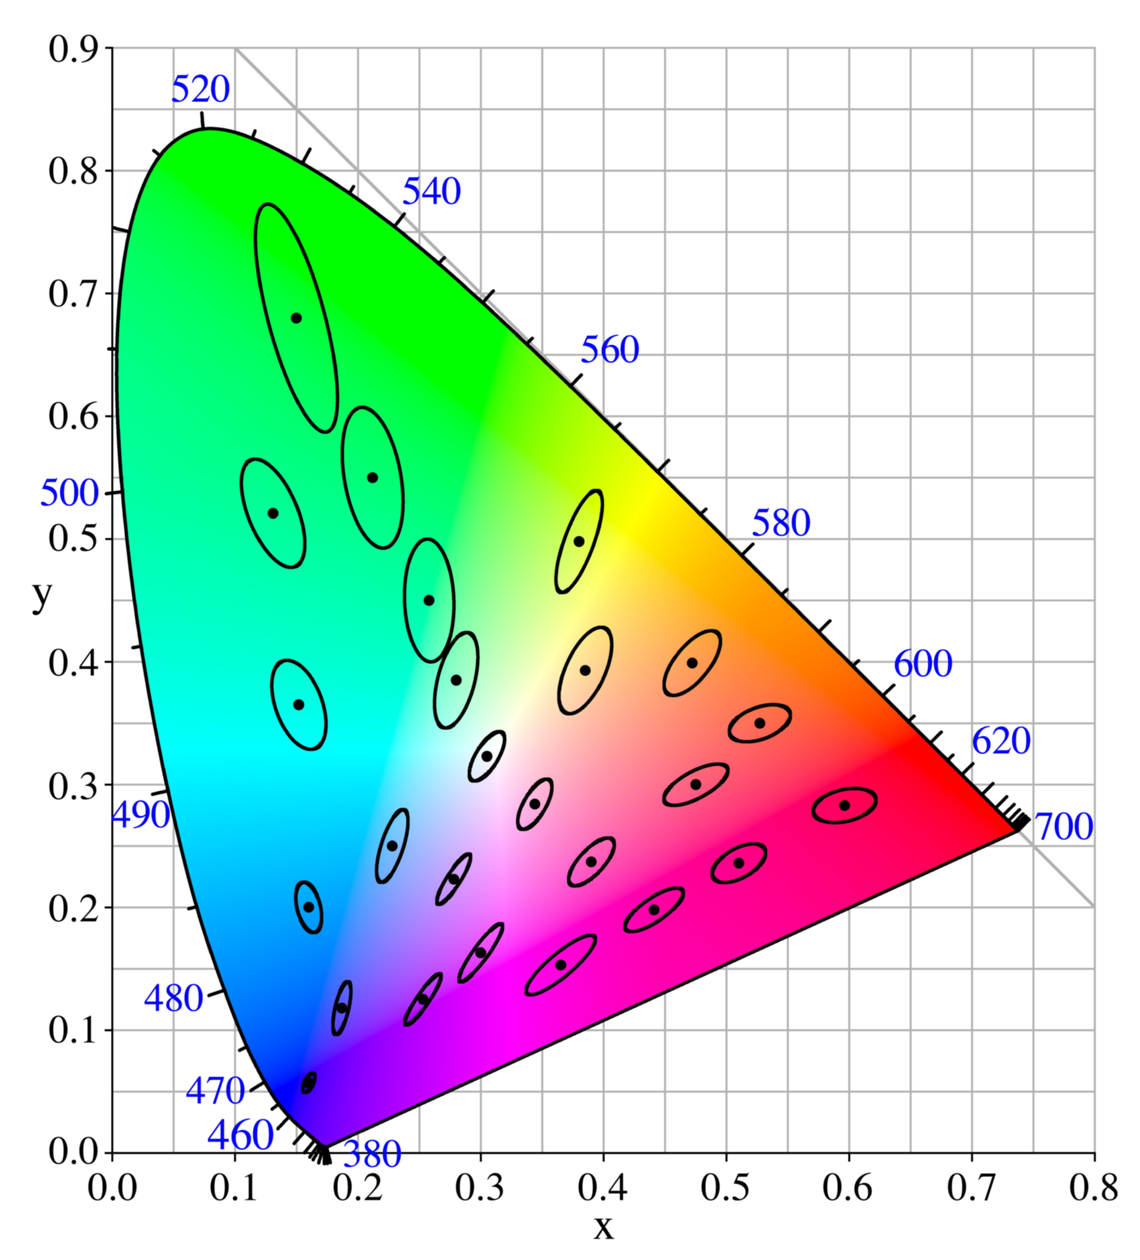
\includegraphics[width=\textwidth]{_external/media/CIExy1931_MacAdam.png}
	\caption{MacAdam ellipses on 1931 standard chromaticity diagram 
		\cite{wiki:macadam:2017}}
	\end{subfigure}
	\begin{subfigure}[t]{.5\textwidth}
		\centering
		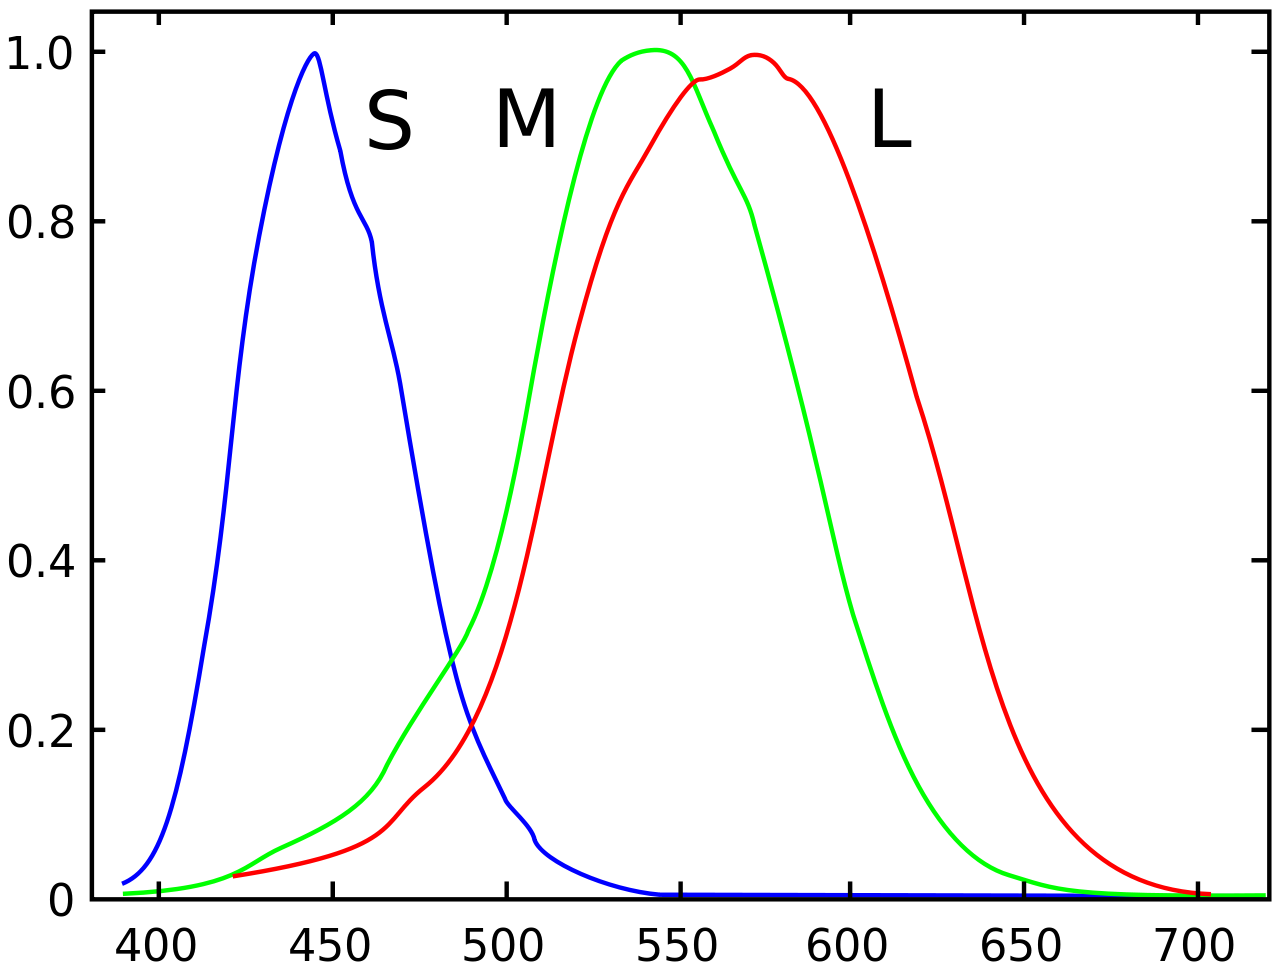
\includegraphics[width=\textwidth]{_external/media/1280px-Cones_SMJ2_E.png}
		\caption{Normalized responsivity spectra of human cone cells, S, M, and 
		L types after Wyszecki et. al \cite{wiki:Wyszecki:2017}}. Notice the 
		overlap between M and L cones.
	\end{subfigure}
\end{figure} \todo{The layout is a bit wonky here.}

Most consumer cameras - and even most production cameras - use dot-matrix 
sensors with a weighted ration of green (4), red (2) and blue (2) pixels, 
called Bayer pattern \cite{kodak:bayer:1976}, giving it - similar to human 
vision - a high color vector space. Green is generally easier to light, 
illuminate and adjust over blue screens. Small irregularities, for example 
through uneven lightning or crinkles in the material, can be adjusted easily by 
the user and allows for a relatively clean camera image generation.
\newline
The quality of input footage makes a big difference in separating back- and 
foreground, hence a well lit and adjusted set is a good backbone for well 
working chroma keying.

\section{What's VR - Differentiation of AR, VR \& MR}

In search of an appropriate abbreviation for computer-enhanced real time 
imagery a recent addition is "XR", where \textit{X} is a letter of your choice. 
Definitions are getting more diluted and generally describe a technique, rather 
than an apparent effect by now.

\begin{figure}[htb]
	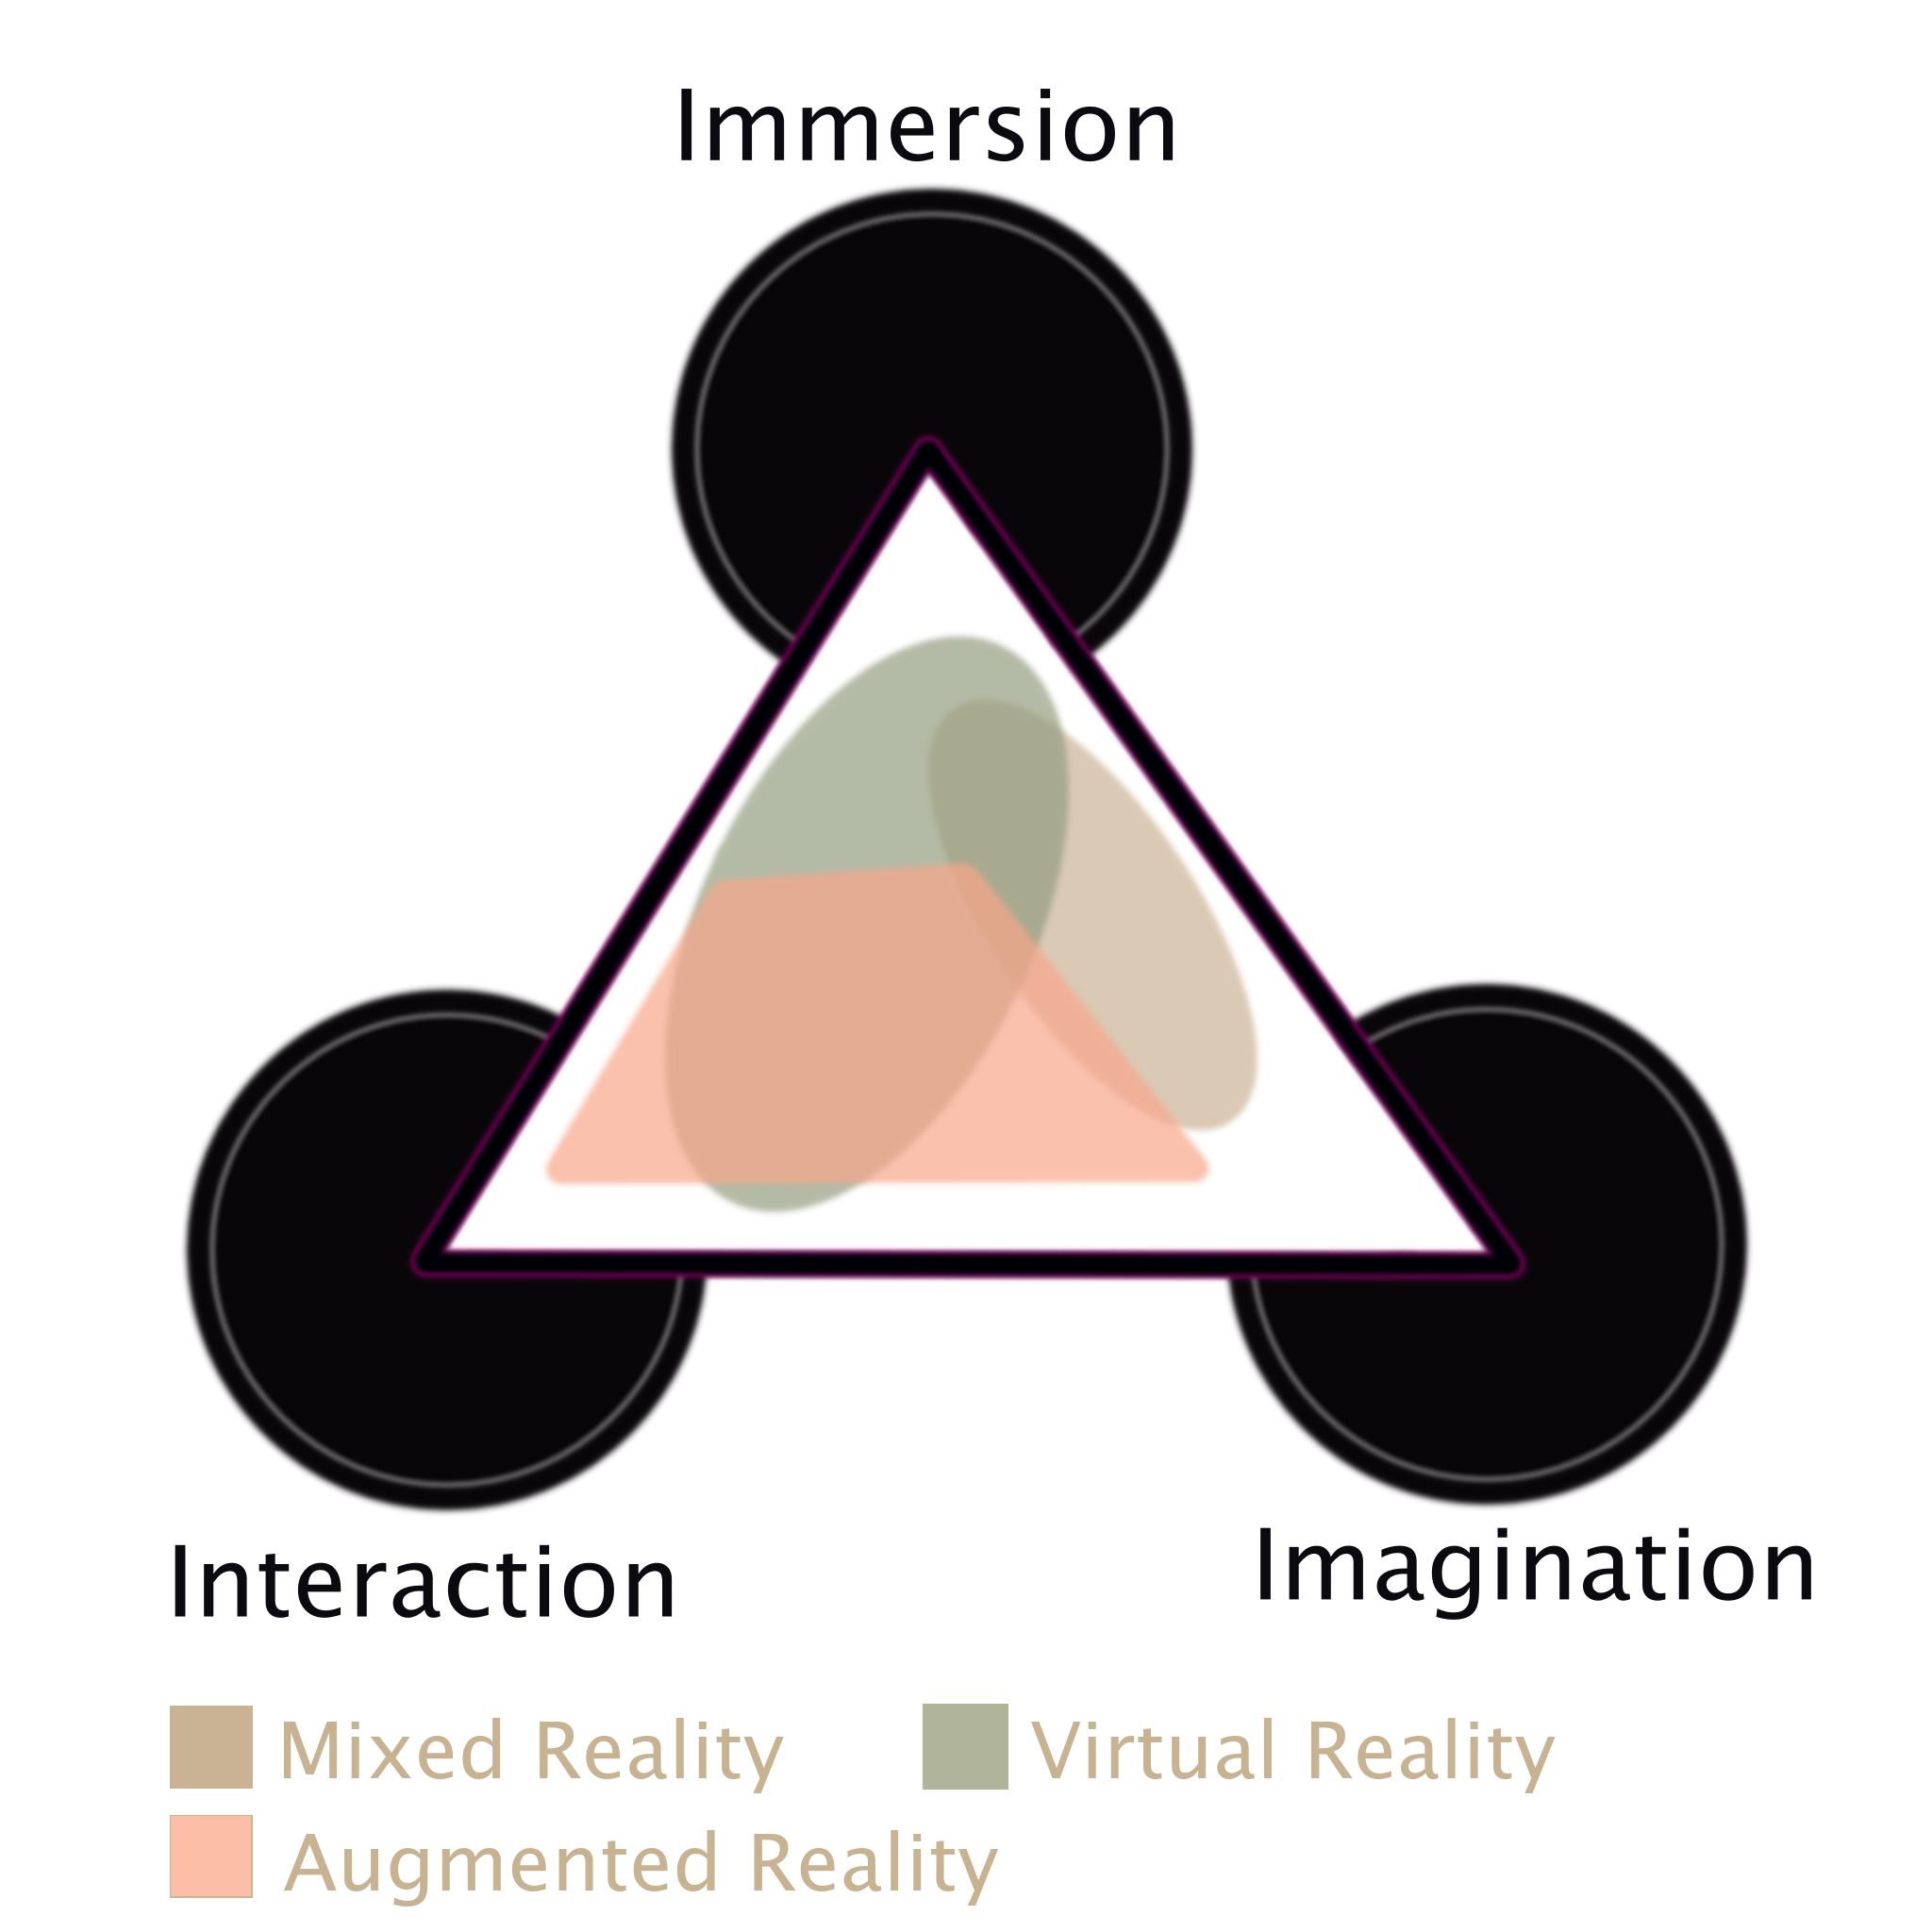
\includegraphics[width=\textwidth]{_raw_resources/i3-triangle.png}
	\caption{I\textsuperscript{3} Triangle - figurative quantization of 
		different reality extending methods}
	\label{fig:xr:i3-triangle}
\end{figure}
Augmented Reality (AR) is a concept by augmenting real world imagery with 
additional information and interactable objects. It used to be called Mixed 
Reality\cite{satoh:case:1998} \cite{tamura:mixed-reality:2001}, merging real 
world imagery with 3D objects but has slowly adapted to AR, since they both 
described the same concept. It ranges from very simple devices displaying data 
in the field of view of an user up to full augmentation, displaying 3D models 
overlaying on real world objects. This can be done ranging from Pepper's Ghost 
projections, augmenting video - a famous example is the rather successful 
"Pokémon GO" -, up to the Microsoft HoloLens, that has sensors for a wide range 
of spatial mapping, spatial anchoring and distant field calculation.

Virtual Reality is a concept usually done by stereo projection of a 3D 
environment inside a Head Mounted Display. It takes an user out of the current 
room and sets him into a complete new, virtual reality - hence its names 
origin. HMD hardware ranges from the simplistic Google Cardboard 
\footnote{using a smart phone as display device} to the Samsung GearVR 
\footnote{similarly uses a smart phone as display driver} up to the Oculus Rift 
and HTC Vive\footnote{which are driven by a mid- to high range PC}. The latter 
two products offer room-scale experiences where an user is able to move freely 
in his play space (basically a tacked bounding volume) and allows for six 
degrees of freedom (\gls{6dof}) tracking.

Mixed Reality is an extension of Virtual Reality, allowing bystanders to get an 
impression of the virtual 3D environment around an actor. By reproducing 
virtual projection parameters of a 3D environment, it is possible to place a 
real world camera feed at the right position inside the 3D scene. This 
yields a combined application of Augmented and Virtual Reality technique. A 
production environment can be achieved with a \gls{6DOF} HMD and additional - 
either user or tracking input for positional and rotational parameters for the 
real world camera. 

\section{Immersion vs. Communication}

\todo[inline]{maybe the overview does already a "good enough" job to bring this 
across.}

Virtual Reality, as previously mentioned in \ref{sec:intro:outline}, is very 
immersive but the experience is hard to imagine without wearing a HMD yourself. 
Additionally doesn't VR offer any ways to allow observers a similar experience 
as the VR actor.
\newline
A very obvious problem starts on interaction. A VR user doesn't always need to 
see his hands to interact with a scene due to the natural way of holding these 
controllers in his hands and directly translating controller interaction to the
virtual environment. However an outside viewer does not see the actors hands 
and will not understand any actions performed by the user if he doesn't see the 
virtual hands. Any usage context that happens off-screen cannot be communicated 
and therefore will be lost.
\newline
A recent game example, Rick and Morty: Virtual Rick-ality, tries to mitigate 
this issue by placing virtual CCTV cameras into the scene, which can be 
controlled through outside observers - giving a neutral third-person view into 
the three-dimensional scene. A VR actor is replaced as a loose avatar 
representing a figure (Morty) from the cartoons universe.
\todo{Add a screenshot of that}

Mixed Reality merges the actors and virtual realities context, allowing outside 
bystanders a comparable window into the actors experienced world. In fact, 
initial promotional material for the HTC Vive showed mixed reality footage, 
produced by one VR computer and a secondary composition PC 
\cite{valve:mr-production:2016}. It's setup is comparable to the one in this 
thesis and differs by composition techniques and by using more than one 
software context, done by outputting a rendered image of the virtual scene and 
compositing it on another system.

\subsection{Evolution of Virtual Reality Footage}

Originally VR footage consisted of the output that was sent to the headset, 
including image transformation that needs to be done to correct the headset 
lenses \footnote{this is referred to as "Barrel Distortion"} - this distorted 
dual image is very hard to follow, as it adds two ambiguous images and has 
additional a high distortion. Since the direct feed to a HMD is used, any 
translation of the headsets position is visible, which results in a jittery and 
unnatural looking motion feed.

\begin{figure}[htbp]
	\label{fig:evolution:steps}
	\begin{subfigure}[t]{.45\textwidth}
		\centering
		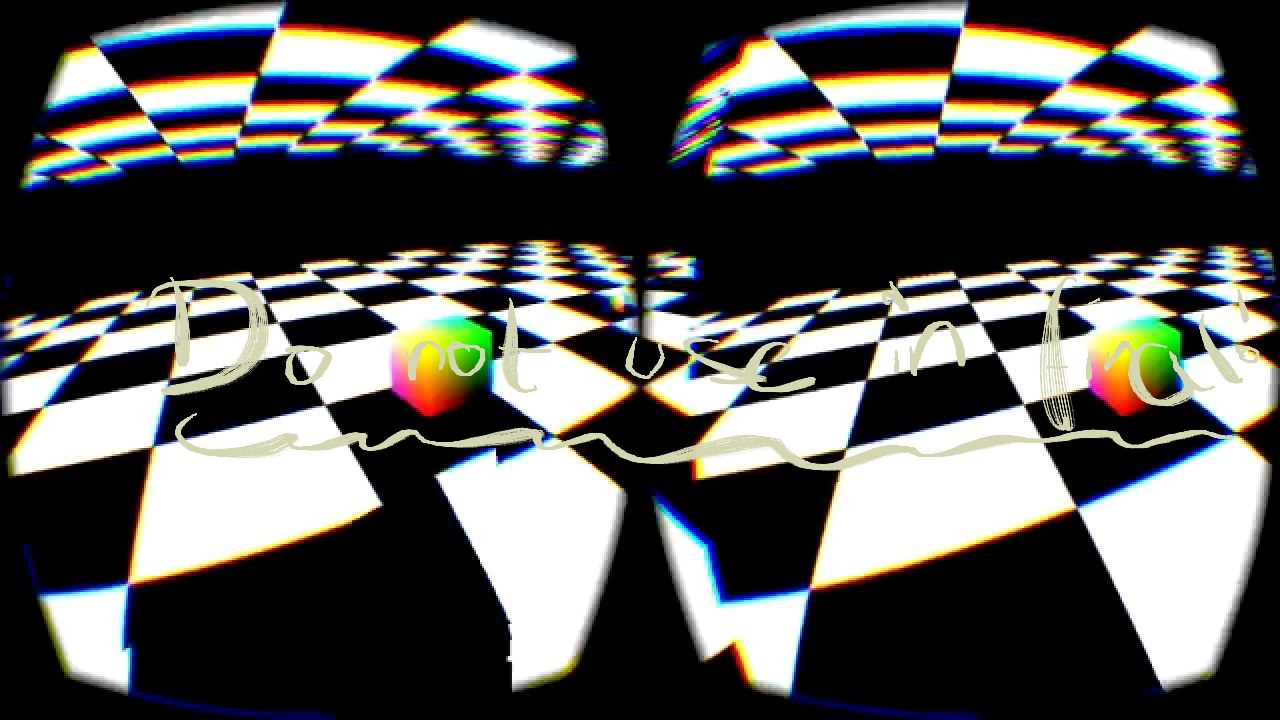
\includegraphics[width=\textwidth]{_raw_resources/lens_distortion.jpeg}
		\caption{Distorted direct dual output to a Oculus DK2.}
	\end{subfigure}
	\begin{subfigure}[t]{.45\textwidth}
		\centering
		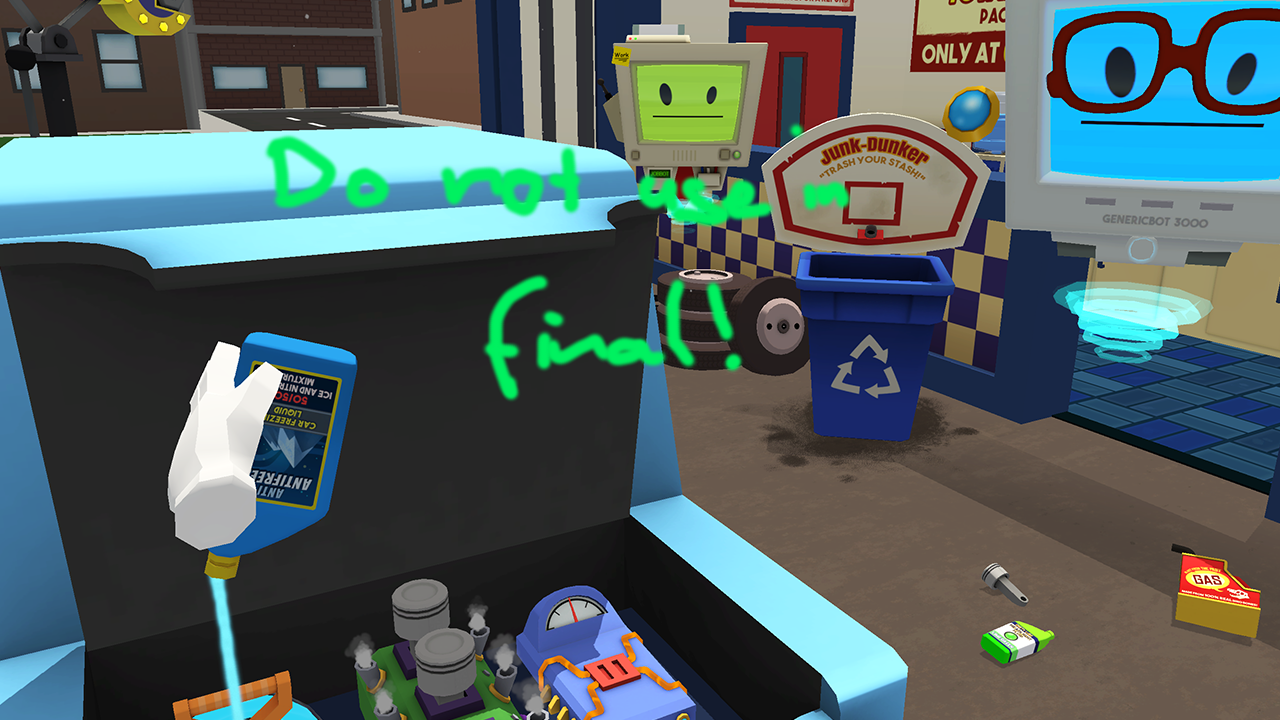
\includegraphics[width=\textwidth]{_raw_resources/job_simulator_vr.png}
		\caption{A first person, single screen output is an improvement, but is 
			hard to follow in motion.}
	\end{subfigure}
	\newline
	\begin{subfigure}[t]{.45\textwidth}
		\centering
		
\includegraphics[width=\textwidth]{_raw_resources/rickality_cctv.png}
		\caption{"Rick and Morty: Virtual Rick-Ality" allows outside observers 
			to control mounted CCTV cameras to observe the actors interaction.}
	\end{subfigure}
	\begin{subfigure}[t]{.45\textwidth}
		\centering
		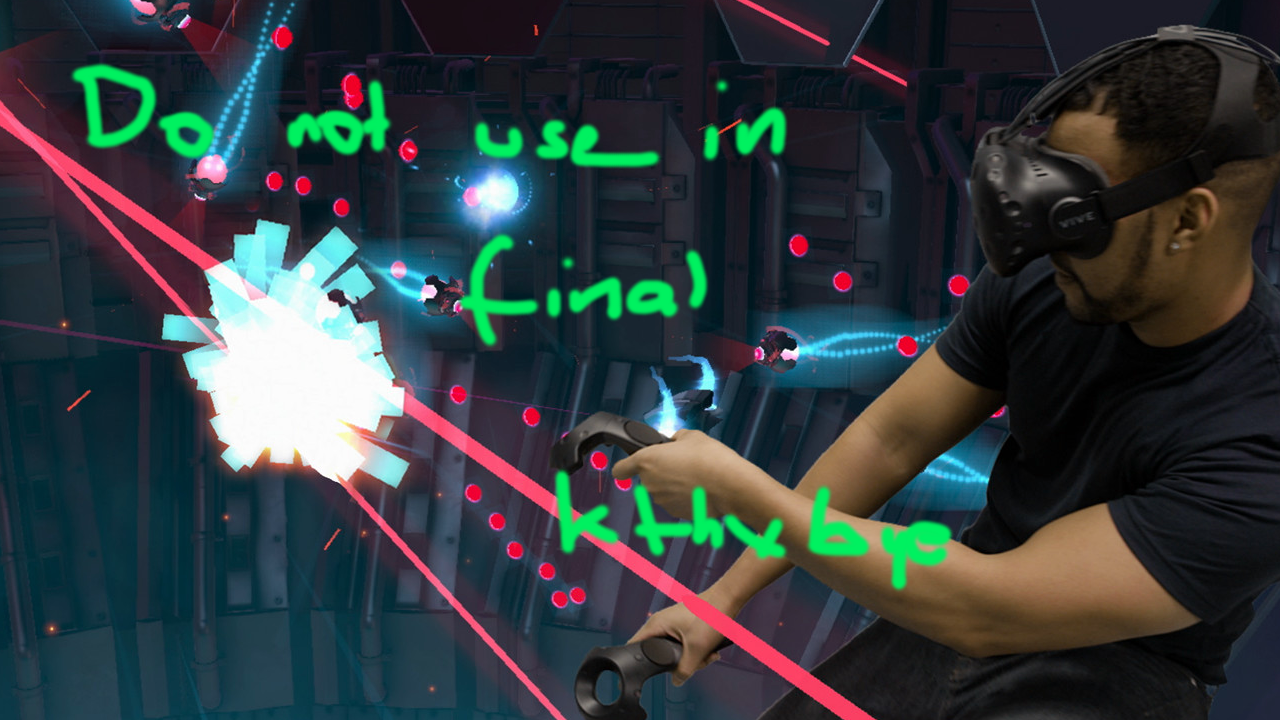
\includegraphics[width=\textwidth]{_raw_resources/the_lab_mr.png}
		\caption{Currently a screenshot of The Lab MR - but actually will be 
			one of my solution. Just gotta take some screenshots.}
	\end{subfigure}
\end{figure}

A next step was to render one eye in fullscreen of the attached monitor and do 
all image transformations (mainly crop and distort) after rendering it, 
allowing bystanders to get a clear first person image of the actors experience. 
Additionally, as a secondary camera, a dampened movement can be set to mitigate 
jittery motion. As previously pointed out, this works but sometimes loses 
interaction context, especially when no hands are visible. 
\newline
Then there is currently only one game, Rick and Morty: Virtual Rick-ality, that 
has an optional CCTV feature enabled, in which third persons can control a 
variety of mounted, virtual cameras and follow the actors interaction with the 
3D environment. This VR actor is then replaced with an avatar to visualize what 
how he is interacting with the scenery.
\todo{Maybe I should pin down the timeline - how long it took for a 
next step to emerge from the medium.}
\newline
Finally there is mixed reality, where the VR actor is placed in context of 
the virtual reality scene. This has been done previously by post-production for 
trailers and allows for a better understanding between virtual interaction and 
real actor motion. With its help it is possible to invite third person viewers 
into the VR experience in a natural way.

\section{Mixed Reality and its use cases}

\todo{There is a meeting planned to discuss A+Cs interest and use cases 
for MR - which then probably ends up in here in a summary.}

\section{Current state of Mixed Reality Production}

There have been an increasing number of presentations for mixed reality setups. 
To sort this thesis into the current scope of production environments, it is 
necessary to look at other approaches and their differences to the proposed 
solution.

\subsection{SteamVR \& Oculus SDK plugins}

Both SteamVR and Oculus SDKs supply plugins to enable mixed reality capturing. 
These system approach the problem similarly by compositing an incoming video 
stream directly at the current position of an registered camera tracker, thus 
failing to accommodate for different input latencies from the motion video 
feed, yielding an inconsistent visual performance. Oculus states on their 
manuals, that these are currently only intended "for proof-of-concept, 
troubleshooting, and hobby use." \ref{oculus:mr-setup:2017}
\newline
In addition SteamVRs solution supports only video-output composition with a 4K 
HDMI output - which in turn means that the signal has to be captured on an 
external device and has to be composited on a secondary system. The 
configuration parameters are "barebones" at best and yielding good results is a 
matter of the best possible studio setup capture.

\subsection{Fantastic Contraption}

The game "Fantastic Contraption" from 2016 allows livestreamers to do a video 
composition for mixed reality. While this approach allows to mitigate video 
input delays it cannot have a free moving camera with an additional motion 
tracker.
\newline
"Fantastic Contraptions" trailers also show another approach by replacing the 
actor with an avatar by basically rendering a certain depth and then placing 
real world camera footage as background. With such a system any live video 
background removal is not necessary and real world footage of the actor is 
lost. The games trailer composition has been achieved in post production. 
\cite{gartner:cinematography:2017}

\subsection{Owlchemy Labs Mixed Reality}

Owlchemy Labs is a VR game developer located in Austin, Texas. They're working 
on VR experiments and use similar techniques discussed in this paper. Their key 
difference in visual reproduction is by using a stereoscopic camera to record 
an actor and can reproduce the actors depth per pixel, allowing for more 
complex fore- and background separation for a more accurate visual reproduction.
\newline
While Owlchemy Labs announced real time mixed reality compositing, there hasn't 
been a shipped product or update for one of their games that allows for live 
mixed reality capture. \todo{Sauce!11!}

\subsection{Apple Keynote}

Apple presented a real time mixed reality showcase done on their computer 
systems on their annual keynote "WWDC17". It is driven by Unreal Engine and 
uses also similar techniques as discussed in this thesis. That presentation is 
currently the best live performance of mixed reality with a high quality chroma 
keying, depth reconstruction and high fidelity graphics. There is no technical 
information available yet. \todo{Gimme that sauce, at least 'ze video!}
% !TeX spellcheck = en_US
% !TEX root = ../thesis-example.tex
%
\chapter{System Setup}
\label{ch:system-setup}

The following section describes the hard- and software components used for the 
thesis and results. All demonstrations have been performed on that environment. 
All dependencies have been explicitly marked to allow a similar, but not exact, 
setup to reproduce these results.

\begin{figure}[htb]
	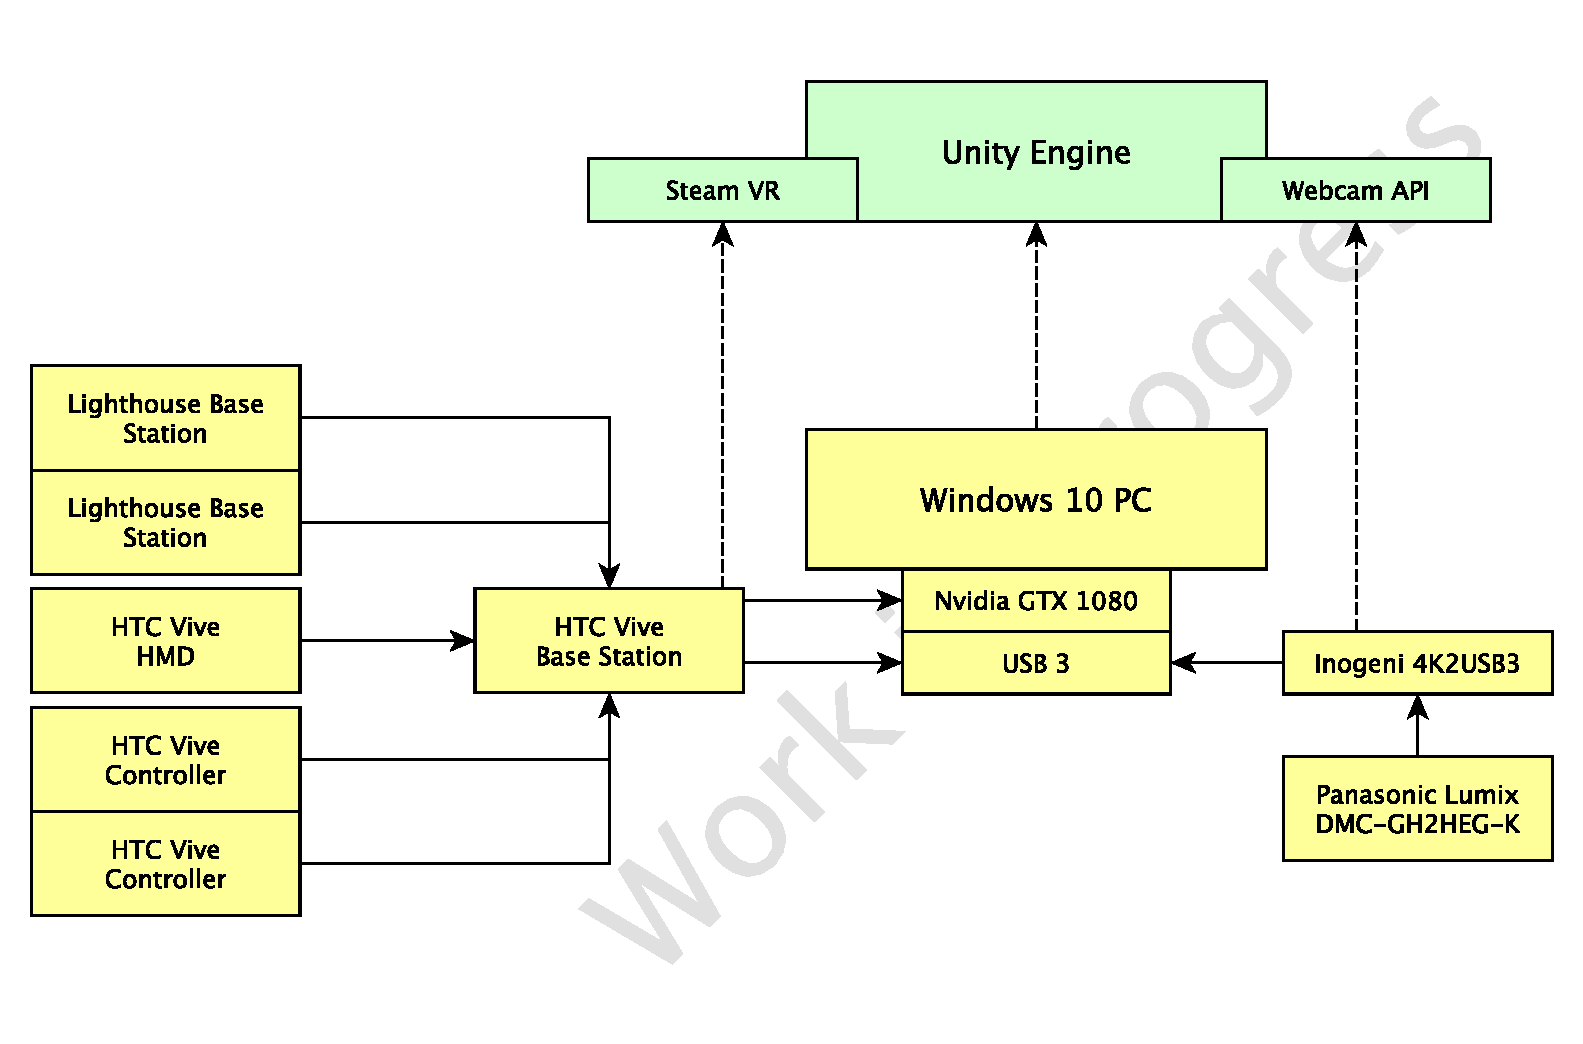
\includegraphics[width=\textwidth]{gfx/System-Components}
	\caption{Diagram of hard- and software components.}
	\label{fig:system-components}
\end{figure}

\section{Hardware Configuration}
\label{sec:hardware-config}

The hardware configuration is split in three main parts:
\begin{my_list}
	\item Windows PC Workstation
	\item Virtual Reality Tracking Solution
	\item Motion Video Input Feed
\end{my_list}

Each individual configuration is basically interchangeable with other systems, 
as long as predefined conditions are met. Each condition is listed first in 
each subsection.

\subsection{PC Workstation}

As the software is built in the Unity Engine, the workstation is limited to 
either Windows or Mac OS X systems the only requirement - besides being 
powerful enough to render the 3D scenes - is two USB3 ports to ensure enough 
data throughput for the video and virtual reality solution, as well as two 
video outputs for a monitor and its headset.
\newline
The configuration used for this thesis is:
\begin{lstlisting}
	CPU: Intel i7-6700 @ 3.40 GHz
	RAM: 16GB DDR4
	GPU: Nvidia Geforce GTX 1080
	System: Windows 10 v. 1703
	Engine: Unity 5.6f3
\end{lstlisting}

This system configuration is to date a high-end workstation that has an 
abundance of render performance and memory for complex and taxing computations 
that have to be performed for a mixed reality composition.

\subsection{Inogeni 4K2USB3 Capture Device}
The Ingoeni 4K2USB3 converter is a standalone box that allows to receive any 
HDMI source and converts it as a webcam video feed usable by "plug'n'play" 
device management of Windows. It's advantage is that it enables any HMDI source 
to be usable as system webcam, thus enabling and arbitrary choice of video 
cameras and a very simple integration with any software through the systems 
provided webcam API. With help of the converter box it's possible to request a 
webcam as video resource and process that video feed as a texture on the GPU.

\subsection{Panasonic GH2 System Camera}
This camera provides a direct video feed via HDMI with low latency. It can 
directly feed into the Inogeni 4K2USB3 and produces a stable, high quality 
video feed with a low signal to noise ratio in well lit environments. 
Additionally it has a well sized photo sensor allowing the camera to capture 
singular frames with reduced motion blur.

\subsection{HTC Vive with Controllers and Lighthouses}
The currently best virtual reality and tracking device available to the public 
is the HTC Vive. It includes two infrared sending stations called "Lighthouse", 
two Vive Controllers\footnote{often delightfully called "Wands" due to its 
controllers design} and a headset. Both, headset and controller systems, are 
enabled with 6 degrees of freedom (6DOF) tracking. The tracking system is a 
black box, in which only the transformation matrices for the hand controllers 
and the HMD can be accessed\footnote{as well as sensor input data from the 
controllers}, which already have been processed by the additional SteamVR 
software. By default this transformation has a normalized length of 1 unit to 1 
meter. Designing scenery and sense of size is therefore rather imaginable. The 
data provisioning is done by a library called "SteamVR for Unity", which makes 
the usage of said matrices in engine fully transparent.

\subsection{Vive Controller Tripod Mount}
Most cameras have a standardized way of mounting tripods. Since the Vive  
controllers have no reference plane. Minuscule differences in mounting angles 
change the projection parameters to noticeable effects, so it was necessary to 
build a mount for the camera to keep controller and video equipment 
transformation synchronized.

\begin{figure}[htb]
	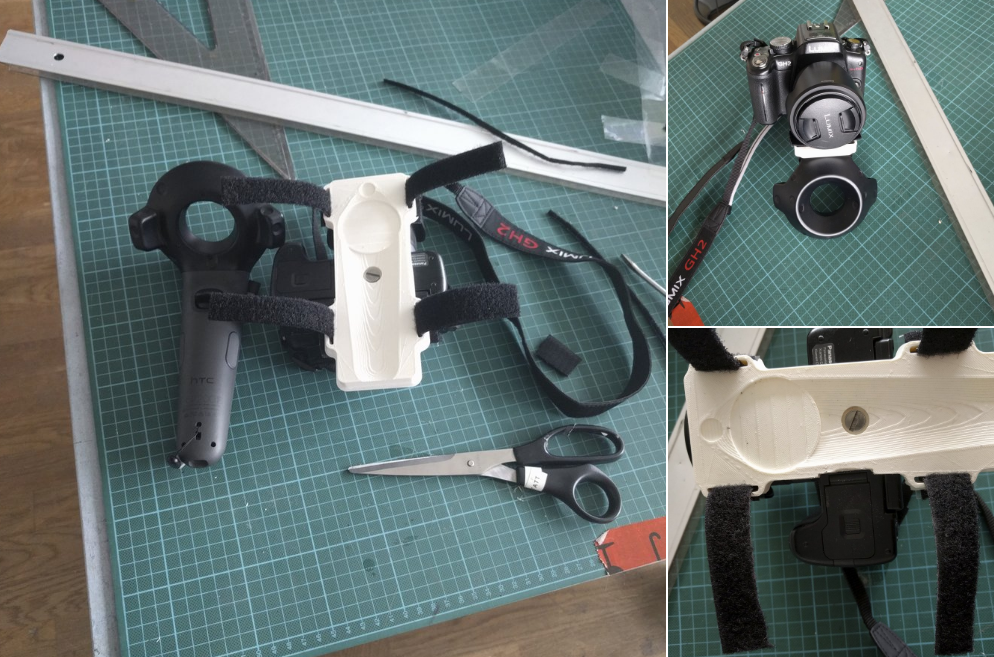
\includegraphics[width=\textwidth]{_raw_resources/ViveStrap-Mount.png}
	\caption{Camera mount for a HTC Vive controller, mounted on the cameras 
		tripod mount}
	\label{fig:system:camera-mount}
\end{figure}

I've built a mount that fits on tripod attachment points and keeps the 
controller locked in the same rotation and position (see figure 
\ref{fig:system:camera-mount}).



\section{Software}

The software of choice is Unity3D, which is a free game engine for students, 
non-profit organizations and small studios. It provides an easy introduction to 
game / 3D engine programming and has a huge development community. While it is 
not the technologically most advanced engine, its fairly easy usage and fast 
development cycles make it a great tool for a bachelor thesis.
\newline
Thankfully, the high abstraction of system APIs means that cross-platform 
development only needs a single code base and makes excruciating tasks like 
webcam access simple - so much so that it boils down to one line of code. 
However, this has drawbacks in overall performance, partially introduced by the 
engine's garbage collection, which are no issue for the used system.
\newline
Its weakness is usually API documentation and - on the downside, too - high 
abstraction levels from most APIs. For example, Unity relies on its own shading 
language which cross-compiles to HLSL, OpenGL and WebGL - this leads to 
problems in buffer and data management, which cannot be controlled well inside 
its render loop.

The software discussed in this thesis integrates and depends additionally on 
SteamVR, a library for Unity, providing the necessary tracking data in the 
engine. SteamVR is developed by Valve, the software is available for free on 
Steam, the complementary library is hosted on GitHub. As of writing this 
thesis, SteamVR is available for Windows and Mac OS X and the software of this 
thesis works on both systems. 

There are no further dependencies or external libraries used.
% !TeX spellcheck = en_US
% !TEX root = ../thesis-example.tex
%
\chapter{From Video to Mixed Reality}
\label{chap:video2mr}

To achieve a real-time rendering environment, as previously mentioned, there 
are two main production cycles. The one discussed in this thesis resolves this 
problem by staying inside one application with multiple render operations per 
frame, the other will be briefly mentioned in the related work section below. 
\newline
The first and most important render cycle is the stereoscopic output of the 
Vive HMD, which has a set frame rate of either 45 or 90 frames per second - 
this is a hard limitation by the providing library, which stalls Unity's 
rendering if a render cycle is above $11ms = 1s / 90$. It is important to have 
consistent performance, otherwise the experience for an actor with the HMD will 
be terribly degraded. This will influence a mixed reality composition, since 
frame rate targets should be evaluated early in production to fit the 
composition environment. Since the render pipeline is mostly affected by GPU 
performance, high fidelity graphics can be achieved with later iterations of 
graphical hardware. Also recent history has shown that different instancing and 
render methods can yield massive performance gains and will likely improve in 
the future of VR\cite{oculus:improv-render:2016}.
\newline
After rendering a stereoscopic image to the HMD another, secondary render cycle 
has to be done on the same frame, which is an in-engine camera inside the 
virtual scene and the relative position of the real-world HMD and real-world 
camera. Since the SteamVR library for the HTC Vive already exposes a 
normalized, synchronized device tracking, it is easily possible to position the 
in-engine camera at an accurate location of the real world capturing device. 
This positional and rotational data is achieved by strapping a HTC Vive 
Controller (or HTC Vive Tracker) to the real world camera and adding another 
transform to the in-engine render camera to allow for an offset, which is 
yielded to the difference between sensor location of the video capturing device 
and the tracking center of a controller / tracker.

\begin{figure}[htb]
	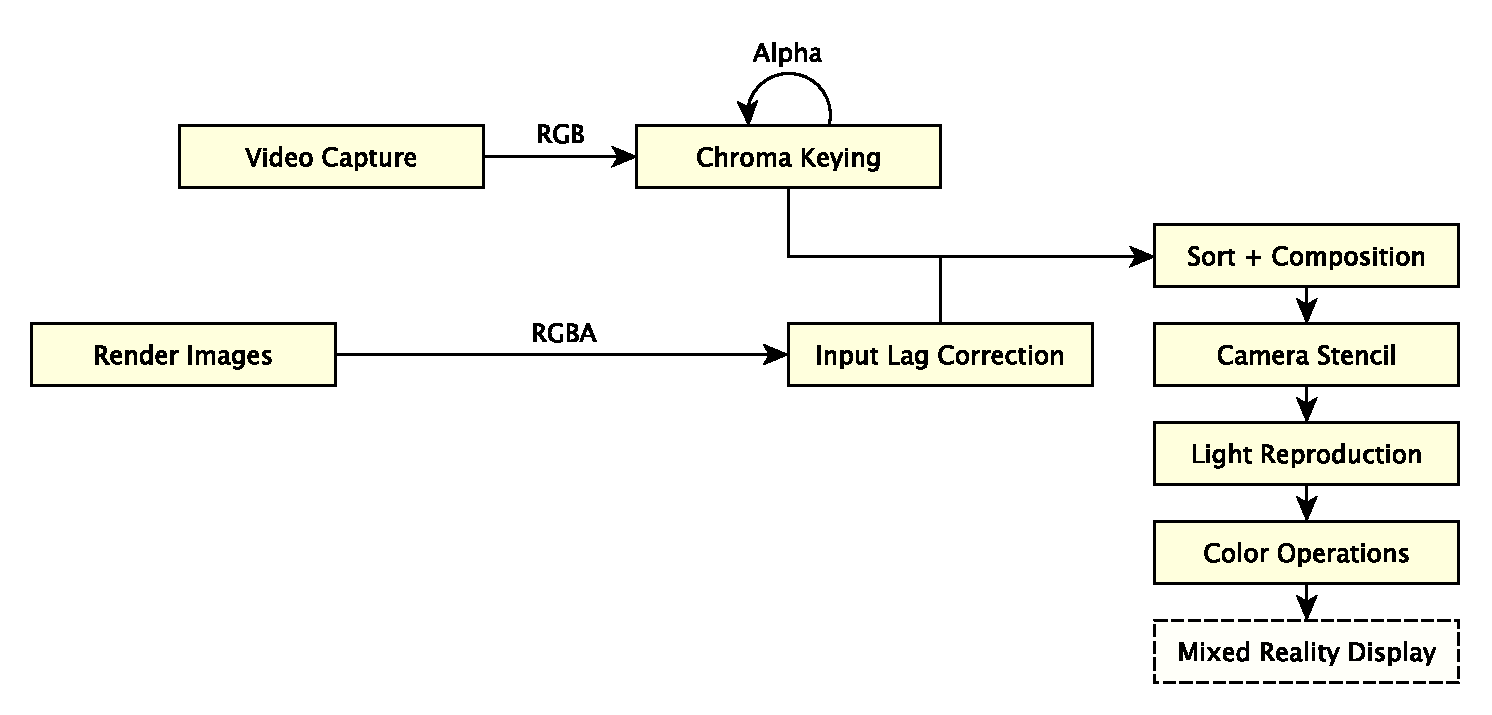
\includegraphics[width=\textwidth]{_raw_resources/pipeline_steps/4_0_pipeline.pdf}
	\caption{Full mixed reality graphics pipeline in order of graphical 
	fidelity impact}
	\label{fig:steps:pipeline}
\end{figure}

The following chapter describes the techniques used to transform motion video 
inside a green screen into a mixed reality image. As brief overview, the steps 
required are performed in order of biggest impact in graphical fidelity (Fig. 
\ref{fig:steps:pipeline}) for the composition of a real world motion video 
feed. This is different to the actual render order but gives a better 
understanding of the techniques used to achieve a mixed reality imagery. A 
closing remark with the order of calculation has been added at the end of the 
chapter.

% !TeX spellcheck = en_US
% !TEX root = ../thesis-example.tex
%
\section{Chroma Key}
\label{sec:chromakey}

Beginning from a real-world camera, the video signal travels through the 
Inogeni 4KUSB3 converter and is accessible with the systems API for webcams. 
(See figure \ref{fig:system-components})

\begin{figure}[htb]
	\centering
	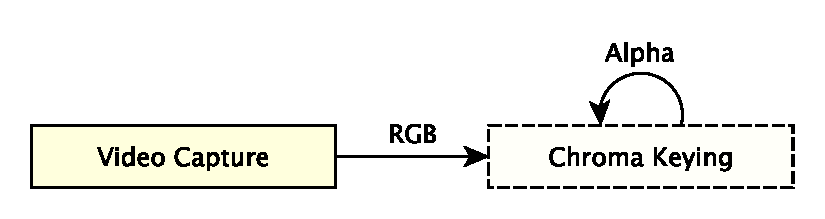
\includegraphics[width=.7\textwidth]{gfx/pipeline/4_1_chroma.pdf}
	\caption{Initial step upon receiving the camera image}
	\label{fig:steps:chroma}
\end{figure}

The initial step is to remove the green (or blue) background from the image, 
which should be live footage of a green (or blue) box. Other literature usually 
refers to it as "pulling a video matte" or "chroma keying." For a reference 
green, there has to be a color picked manually in the material editor of Unity 
--- this was made by a checkbox to show raw output from the camera (eg. fig. 
\ref{fig:chroma:editor}). Then an average green from the background box can be 
picked. This is an important setup step, since lightning situations can vary 
greatly and minor differences in light setups can have a great effect on the 
outcome of visible green background captured by the camera, thus making a 
recalibration necessary.

\begin{figure}[htb]
	\centering
	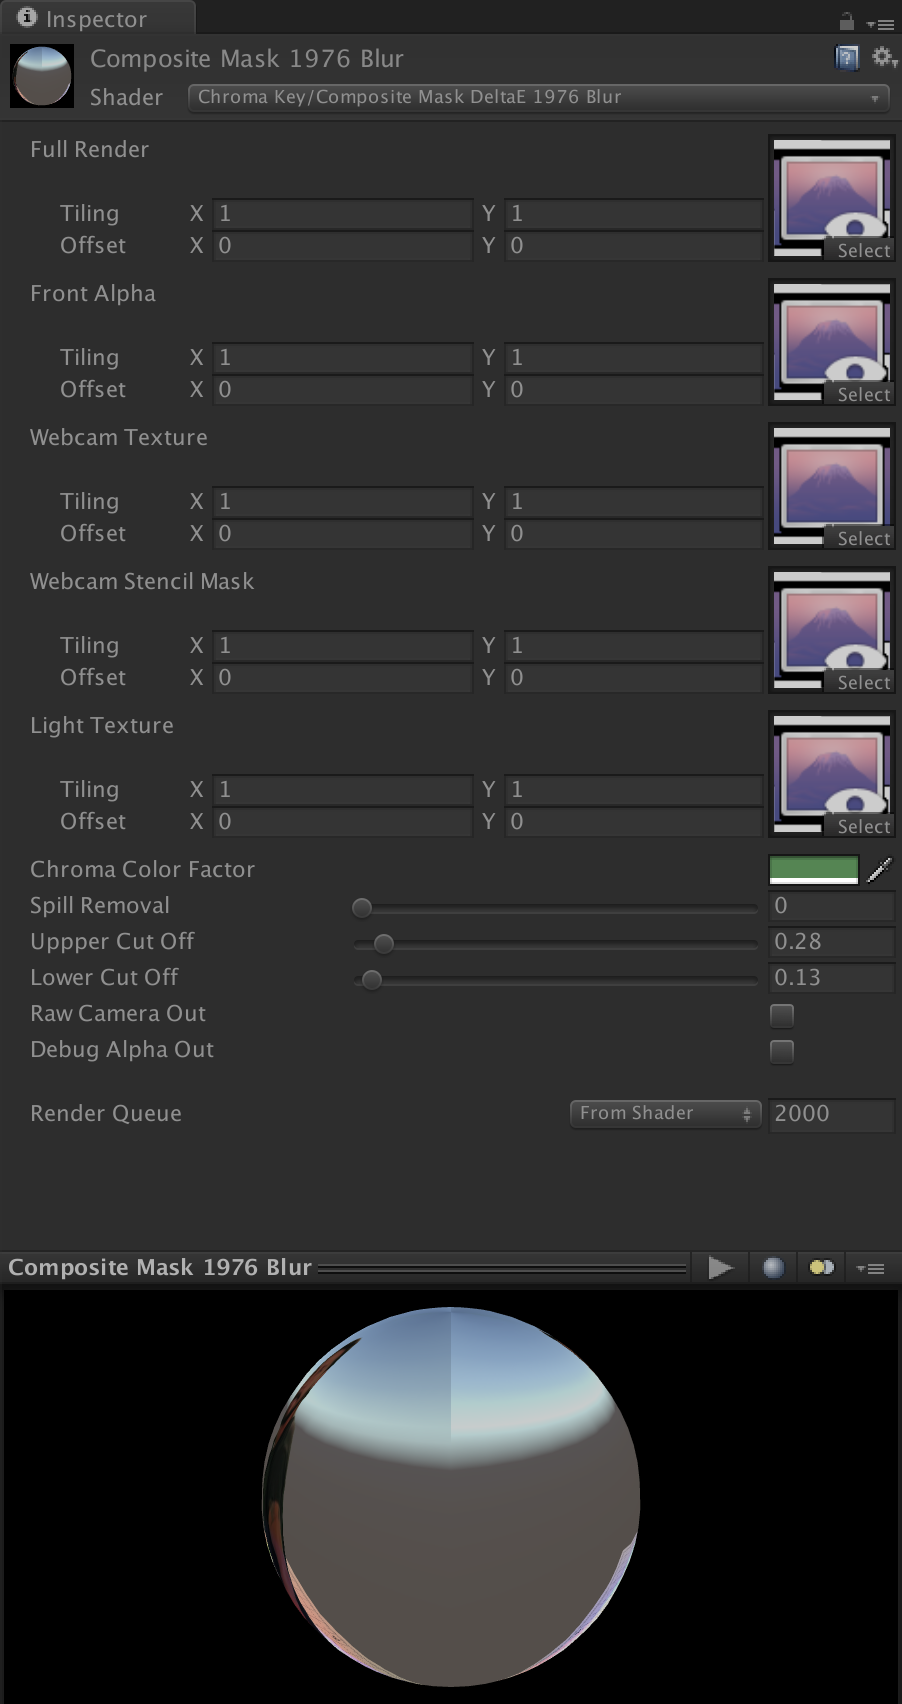
\includegraphics[width=.45\textwidth]{gfx/distances/material-editor.png}
	\caption{Material Editor inside Unity}
	\label{fig:chroma:editor}
\end{figure}

An extreme example case is used for comparing different chroma keying variants, 
which shows high motion blur due to a low shutter speed of the capturing 
camera and fast movement of the depicted actor:

\begin{figure}[htb]
	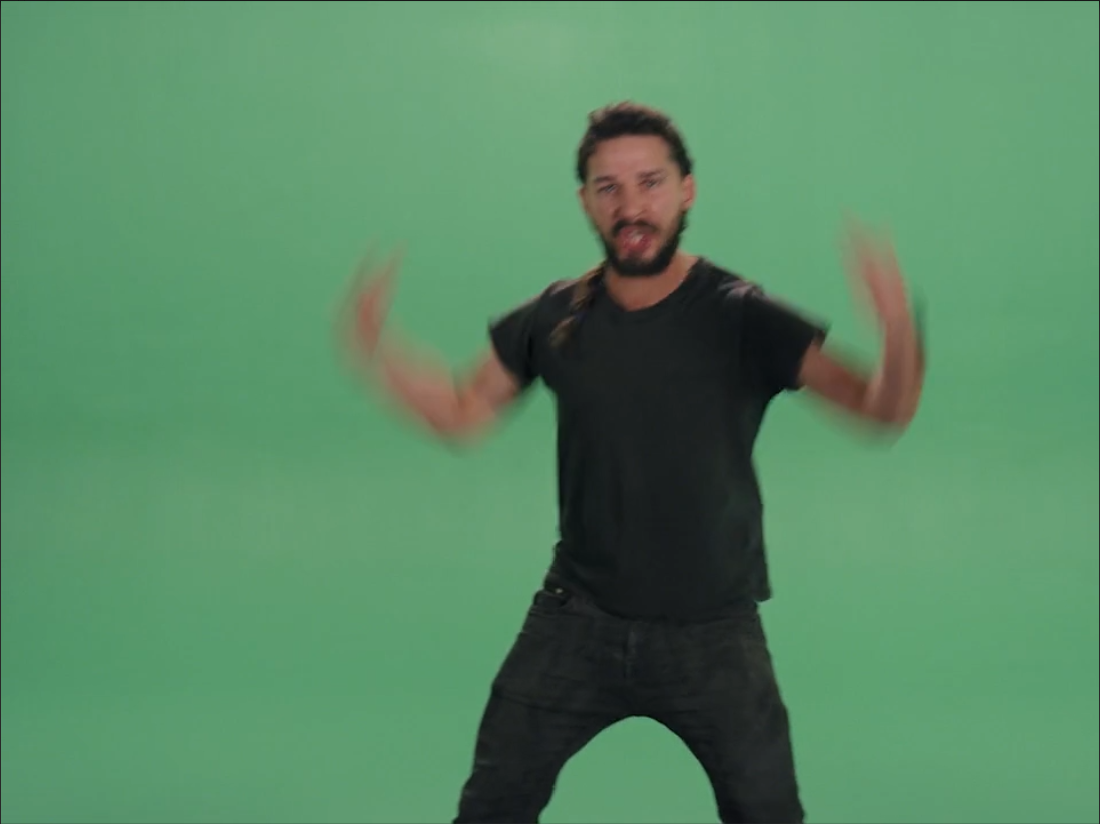
\includegraphics[width=\textwidth]{gfx/distances/example.png}
	\caption{Comparison Image \cite{vimeo:shia:2015} --- sRGB Output}
	\label{fig:chroma:color}
\end{figure}

\subsection{Initial Assumption}

Each RGB color can be represented as a discrete 3-Vector of (red, green and 
blue)  values in range of $[0, 1]$\footnote{Software RGBA color representations 
usually take 8bit per color channel and map between $[0, 255]$ --- graphic 
computing usually maps between $[0, 1]$}. An interpolation between two colors 
can be summarized as a matting equation as follows, where a foreground image 
$C_F$ and a background image $C_B - \alpha_B$ is assumed to be $1$:

\eq{eq:chroma:assumption:alpha:1}{
	I_{x, y} = \alpha_{x, y} C_{F_{x, y}} + (1 - \alpha_{x, y}) C_{B_{x, y}}
}

This matting equation has to be generalized for a later step, where 
$\protect\alpha$ is a value between [0, 1] on fore- and background, yielding a 
total Alpha of $\alpha_T$ as following:

\eq{eq:chroma:assumption:alpha:weak}{
	\alpha_T = \alpha_B * (1 - \alpha_F) \\
}

thus:

\eq{eq:chroma:assumption:alpha:cont}{
	I_{x, y} = (1 - \alpha_T) F_{x, y} + \alpha_T B{x, y}
}

This equation can take $\alpha_T < 1$ into account, which is needed later when 
fore- and background of the virtual environment are merged with a layer in 
between that results from the real world capture.

\subsection{Euclidean RGB Distance}
Assuming a source pixel color $C_S$ and a reference color $C_R$ we can 
calculate the euclidean distance between these two color vectors:
\eq{eq:euclidianrgb}{
	\alpha = \sqrt{(C_RR - C_SR)^2 + (C_RG - C_SG)^2 + (C_RB - C_SB)^2}
}

\begin{figure}[htb]
	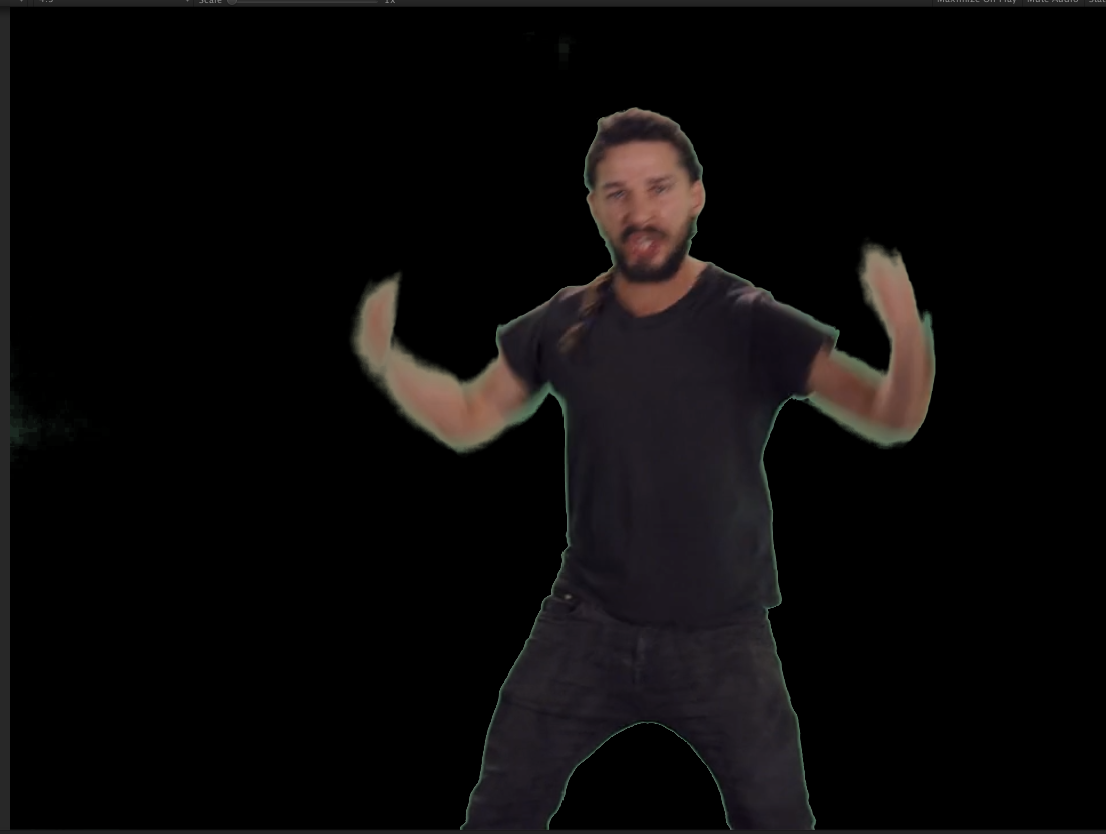
\includegraphics[width=\textwidth]{gfx/distances/chroma-rgb.png}
	\caption{Chroma Keying by using euclidean RGB distance}
	\label{fig:chroma:euclidean:rgb}
\end{figure}

This is computationally very low cost and works well enough to detect a 
difference between two distinct colors. It fails to accommodate for coloring 
that is perceived as different, but tinted by the reference colors. Since the 
green screen material will never achieve 0\% reflectivity, some color will 
spill onto the filmed actor and will therefore generate unwanted chroma-keying 
artifacts, most noticeable on semi-glossy reflection of skin or color tints on 
white clothing.

\subsection{Euclidean YCgCo Distance}

YCgCo gets its name for Luminance (Y), chrominance green (Cg) and chrominance 
orange (Co) and helps decorrelating color spaces by splitting color-lightness 
from color chrominances, thus splicing the color model into brightness and 
color appearance. Since it is a fast, lossless color transformation it 
is used in example for H.264 video encoding and other image compression 
techniques. The two chrominance channels are then split into green to magenta 
and orange to blue color channels and allow for a more accurate distance 
calculation between two colors.

\begin{figure}[htb]
	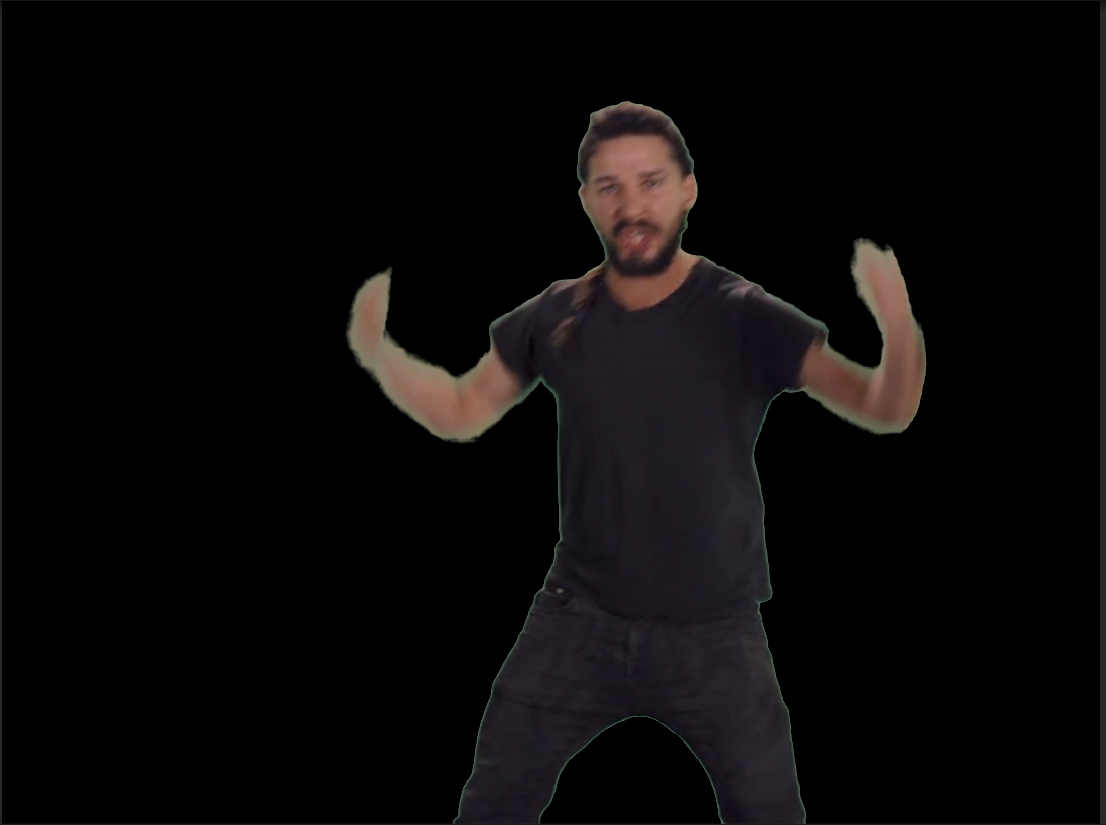
\includegraphics[width=\textwidth]{gfx/distances/chroma-ycgco.png}
	\caption{Chroma Keying by using euclidean YCgCo distance}
	\label{fig:chroma:euclidean:ycgco}
\end{figure}

Transforming any RGB color to YCgCo can be done with a single matrix  
multiplication, which is --- again --- a very low-cost computation on a GPU:

\eq{eq:ycgco:transformation}{
	\begin{bmatrix}
		Y \\
		Cg \\
		Co \\
	\end{bmatrix}
	=
	\begin{bmatrix}
		 \frac{1}{4} && \frac{1}{2} &&  \frac{1}{4} \\
		-\frac{1}{4} && \frac{1}{2} && -\frac{1}{4} \\
		 \frac{1}{2} && 0           && -\frac{1}{2}
	\end{bmatrix}
	*
	\begin{bmatrix}
		R \\
		G \\
		B 
	\end{bmatrix}
}

Given two colors, one from the video source $C_S$ and a reference color $C_R$ 
it is now possible to calculate the euclidean distance on the two chrominance 
channels:

\eq{eq:ycgco:euclidean}{
	\alpha = \sqrt{(C_RCg - C_SCg)^2 + (C_RCo - C_SCo)^2}
}

Due to the increased decorrelation, the result is more accurate and shows less 
artifacts on target pixels, allowing for better matte pulling, less 
green edges and a more continuous, smooth image of an actor.

\subsection{Euclidean Lab Difference}
The International Color Consortium (ICC) defined 1976 \textit{Lab $\Delta$E} as 
a standard model of calculating color differences inside the \textit{Lab} color 
vector volume. The final distance calculation is a linear euclidean scalar as 
with all other models, but accommodates for perceived color differences. It is 
a more expensive computation and needs code branches, which will evaluate all 
branches first by the GPU before using either code path.

A reference white has to be used to convert RGB to the Lab color model to 
accommodate for different RGB color spaces\footnote{which are usually only 
different on stored image material like photos or video}. Luckily the given 
webcam signal defaults to sRGB D65 and does not need a configurable reference 
matrix based on a given color model to handle different RGB color standards.

sRGB conversion needs to be converted to linear RGB while respecting light 
energy per color channel, rather than relative, perceived color brightness: 

\eq{chroma:inversecompanding}{
	v \in \{r, g, b\} \land V \in \{R, G, B\}
}

where: 

\eq{chroma:inverseRGBcompanding}{
	v = \\
	\begin{cases}
		\frac{V}{12.92}                 & \quad \text{if } V \leq 0.0405 \\
		(\frac{V + 0.055}{1.055})^{2.4} & \quad \text{otherwise}
	\end{cases}
}

from there an linear RGB color can be converted to XYZ by the following 
equation:

\eq{chroma:conversioncalc}{
	\begin{bmatrix}
		X\\
		Y\\
		Z\\
	\end{bmatrix}
		=
	\begin{bmatrix}
		M
	\end{bmatrix}
	\begin{bmatrix}
		R\\
		G\\
		B\\
	\end{bmatrix}
}

where:

\eq{chroma:rgbmatrix}{
	\begin{bmatrix}
		M
	\end{bmatrix}
		=
	\begin{bmatrix}
		R X_r && G X_g && B X_b \\
		R Y_r && G Y_g && B Y_b \\
		R Z_r && G Z_g && B Z_b
	\end{bmatrix}
}


\eq{chroma:xyzmatrix}{
		\begin{bmatrix}
		X\\
		Y\\
		Z\\
	\end{bmatrix}
	\begin{bmatrix}
		M
	\end{bmatrix}
	=
	\begin{pmatrix}
		X_r / Y_r && X_g / Y_g && X_b / Y_g \\
		1 && 1 && 1 \\
		\frac{1-X_r-Y_r}{Y_r} && \frac{1-X_g-Y_g}{Y_g} && \frac{1-X_b-Y_b}{Y_b}
	\end{pmatrix}
}

The needed $\begin{bmatrix}M\end{bmatrix}$ for RGB D65 is defined as:

\eq{chroma:sRGBD65}{
	\begin{bmatrix}
		0.4124564 && 0.3575761 && 0.1804375 \\
		0.2126729 && 0.7151522 && 0.0721750 \\
		0.0193339 && 0.1191920 && 0.9503041 \\
	\end{bmatrix}
}

Based on a reference white $U_r \in \{X_r, Y_r, Z_r\}$:

\eq{chroma:xyz2lab:defines}{
	U \in \{X, Y, Z\} \land W \in \{L, a, b\}
}

\eq{chroma:xyz2lab:epsilon}{
	\epsilon = 0.008856 \land \kappa = 903.3
}

where:

\eq{chroma:xyz2lab:ref}{
	w_r = \frac{U}{U_r}
}

\eq{chroma:xyz2lab:channel}{
	f(w) = \\
	\begin{cases}
		\sqrt[3]{w_r}      & \quad \text{if } U > \epsilon \\
		\frac{\kappa w_r + 16}{116} & \quad \text{otherwise}
	\end{cases}
}


\eq{chroma:xyz2lab:conversion}{
	\begin{bmatrix}
		L \\
		a \\
		b \\
	\end{bmatrix}
	=
	\begin{bmatrix}
		116 f_y - 16 \\
		500 (f_x - f_y) \\
		200 (f_y - f_z)
	\end{bmatrix}
}

With this conversion from sRGB to linear RGB to XYZ to Lab we can now calculate 
the euclidian linear distance between two colors $C_S$ and $C_R$, which already 
have been converted to Lab:

\eq{chroma:cie76:distance}{
	\Delta E = \sqrt{(C_R L - C_S L)^2 + (C_R a - C_S a)^2 + (C_R b - C_S b)^2}
}

The resulting values are rated by their perceptive difference (after Mkrzycki 
et. al. \cite{mokrzycki:2012}):

\begin{tabular}[htb]{l | l}
	0.0 \dots 0.5 & the difference is unnoticeable \\
	0.5 \dots 1.0 & the difference is only noticed by an experienced observer \\
	1.0 \dots 2.0 & the difference is also noticed by an unexperienced observer 
	\\
	2.0 \dots 4.0 & the difference is clearly noticeable \\
	4.0 \dots 5.0 & fundamental color difference  \\
	> 5.0 		  & gives the impression that these are two different 
	colors
\end{tabular}

Now it's possible to map alpha values for each pixel based on $\Delta$E 
distances between $m, n$ by clamping and biasing $\Delta$E with a proposed 
"smooth step" algorithm:

\eq{chroma:cie76:clamp}{
	f({\Delta E}) = x = \frac{\Delta E - n}{m - n}
}

\eq{chroma:cie76:min/max}{
	g(f({\Delta E})) = y =
	\begin{cases}
		n        & \quad \text{if } x \leq n \\
		x        & \quad \text{if } n \leq x \leq m \\
		m        & \quad \text{if } m \leq x
	\end{cases}
}

\eq{chroma:cie76:mapping}{
	\alpha(I_{x, y}) = 3 y ^2 - 2 y ^3
}

With that we receive a more natural matte with nearly no green edges, 
continuous actor imagery and smooth alpha transition between actor and green 
screen. Motion blur is hard to account for and is even with professional video 
matting hardware, extensive post production or intrinsic frame matting 
algorithms hard to remove without rough image results.

\begin{figure}[htb]
	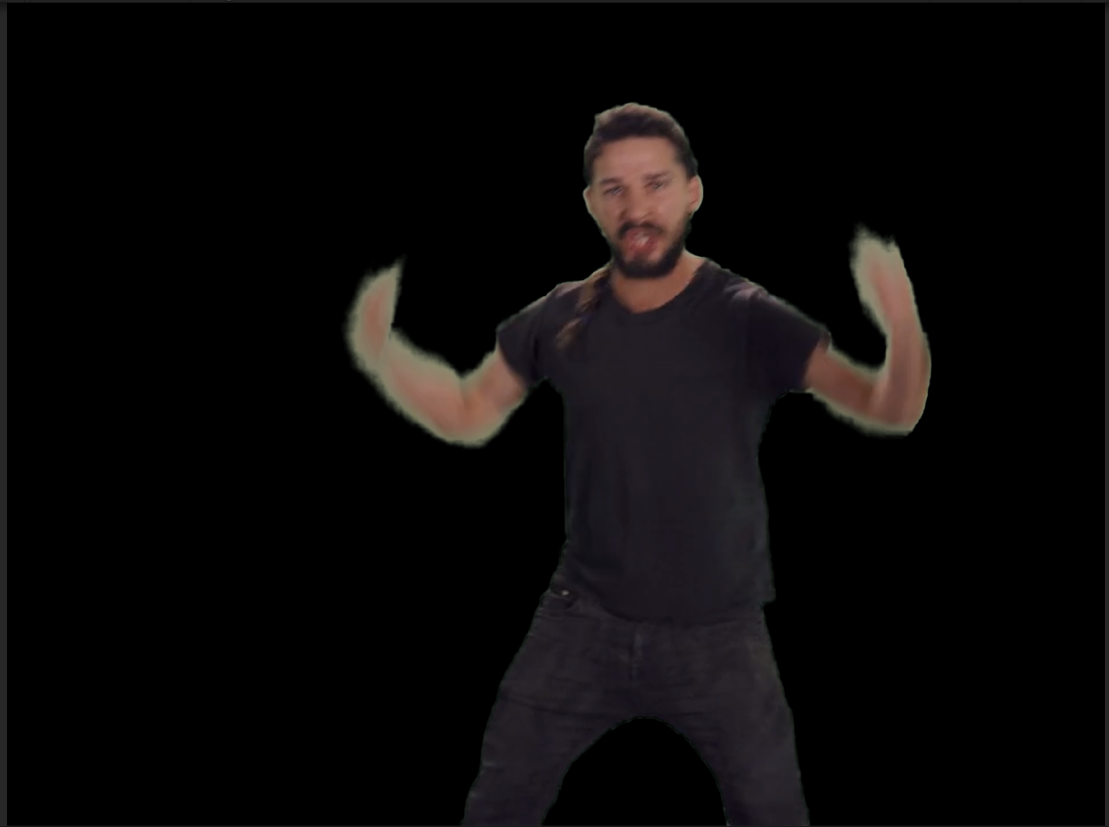
\includegraphics[width=\textwidth]{gfx/distances/chroma-deltae.png}
	\caption{Chroma Keying by using $\protect\Delta $E distance}
	\label{fig:chroma:deltae}
\end{figure}

\subsection{Comparison between Computational Models}

To chose the best variant, balancing runtime and efficiency, there has to be a 
comparison between the presented methods. Again, the previous image will be 
used, since it has complicated color mixing between background and actor. First 
we pick scan line of the image, in this case the 301st row from top, and 
calculate the color distance from each pixel to a reference color $[R, G, B] = 
[0.341, 0.588, 0.42]$.

As seen in figure \ref{fig:chroma:image_comparison}d, CIEDE76s performance is 
significantly better in separating colors and has a broader margin between 
green background and other foreground. This can be observed in figure 
\ref{fig:chroma:image_comparison}, where the scan line is set as background and 
the values are normalized again:

\begin{figure}[htbp]
	\caption{Comparison between different color distance methods}
	\label{fig:chroma:image_comparison}
	\begin{subfigure}[t]{.65\textwidth}
		\centering
		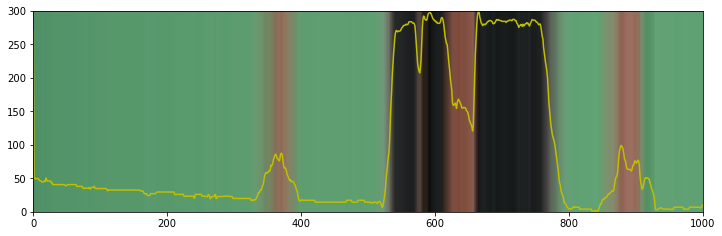
\includegraphics[width=\textwidth]{gfx/distances/color-rgb.png}
		\caption{RGB color distance} 
	\end{subfigure}
	\begin{subfigure}[t]{.3\textwidth}
		\centering
		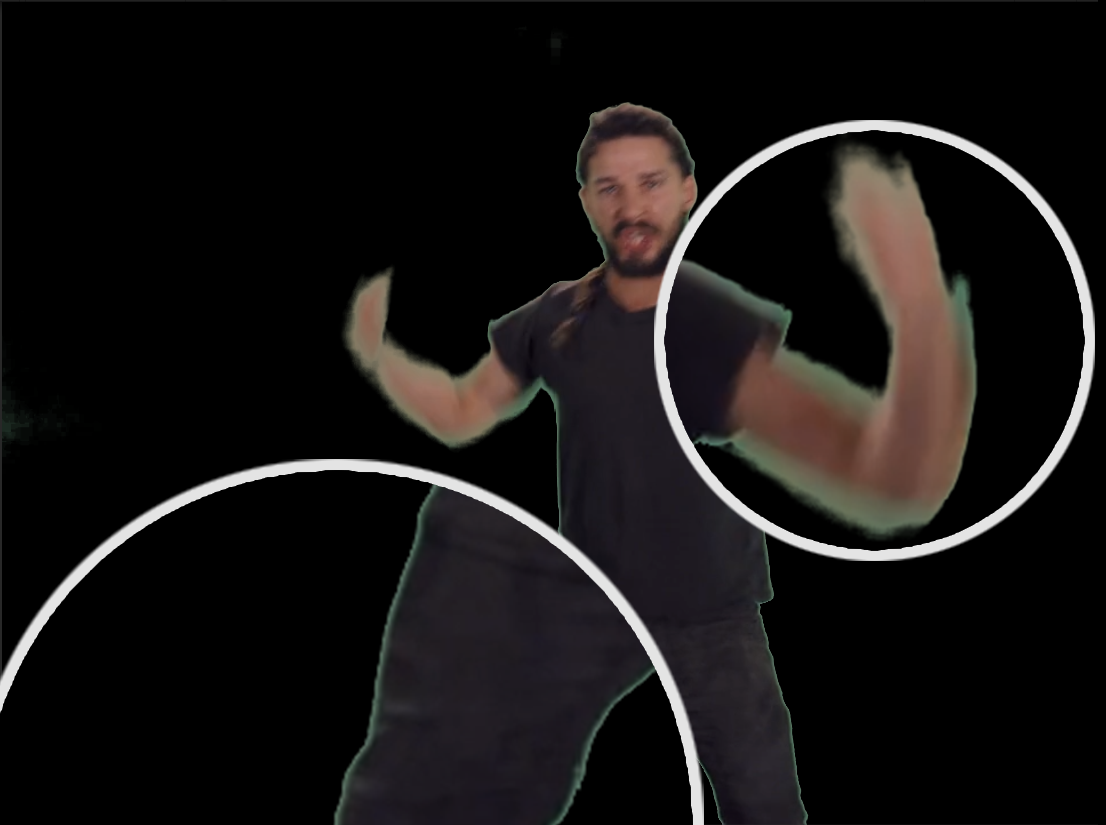
\includegraphics[width=\textwidth]{gfx/distances/zoom-rgb.png}
	\end{subfigure}
	\begin{subfigure}[t]{.65\textwidth}
		\centering
		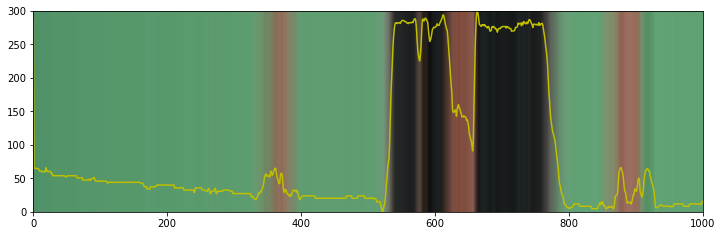
\includegraphics[width=\textwidth]{gfx/distances/color-ycgco.png}
		\caption{YCgCo color distance}
	\end{subfigure}
	\begin{subfigure}[t]{.3\textwidth}
		\centering
		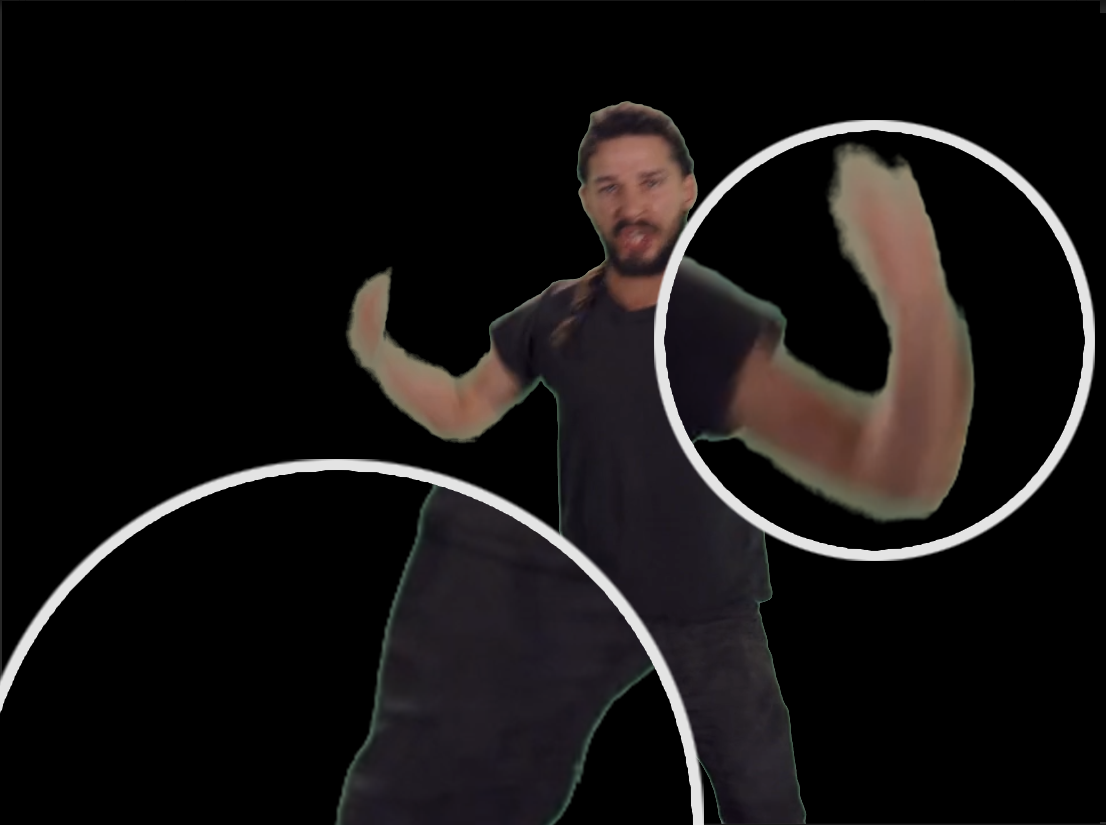
\includegraphics[width=\textwidth]{gfx/distances/zoom-ycgco.png}
	\end{subfigure}
	\begin{subfigure}[t]{.65\textwidth}
		\centering
		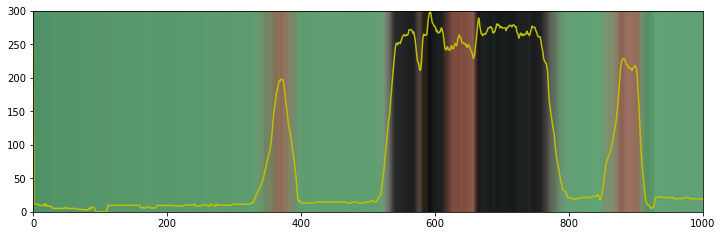
\includegraphics[width=\textwidth]{gfx/distances/color-ciede76.png}
		\caption{CIEDE76 color distance}
	\end{subfigure}
	\begin{subfigure}[t]{.3\textwidth}
		\centering
		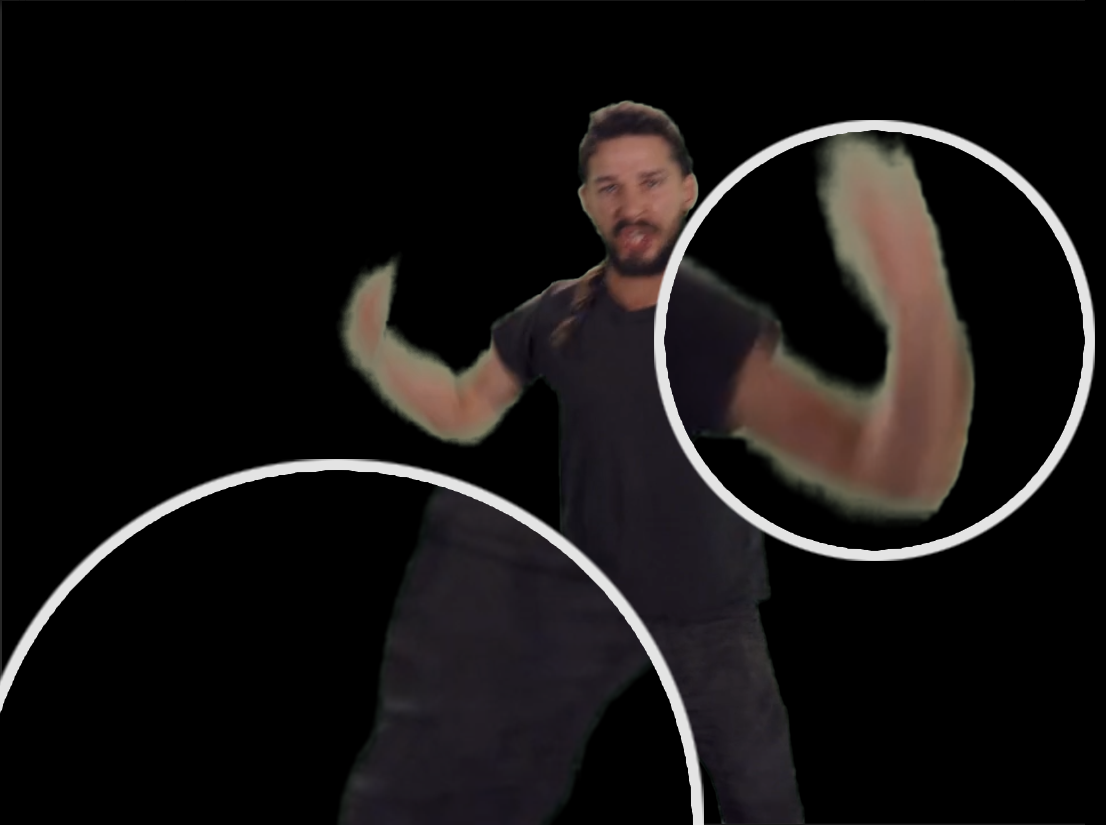
\includegraphics[width=\textwidth]{gfx/distances/zoom-delta_e.png}
	\end{subfigure}
	\begin{subfigure}[t]{\textwidth}
		\centering
		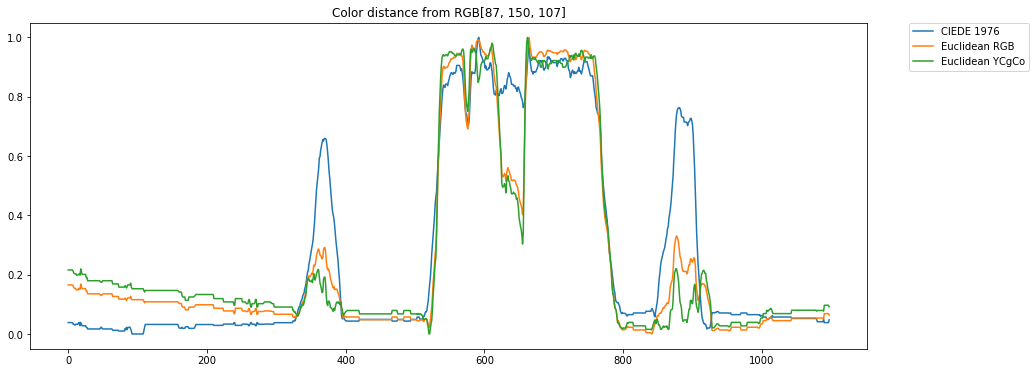
\includegraphics[width=\textwidth]{gfx/distances/dist-comp.png}
		\caption{Normalized graph comparing color difference methods}
	\end{subfigure}
	\begin{subfigure}[t]{\textwidth}
		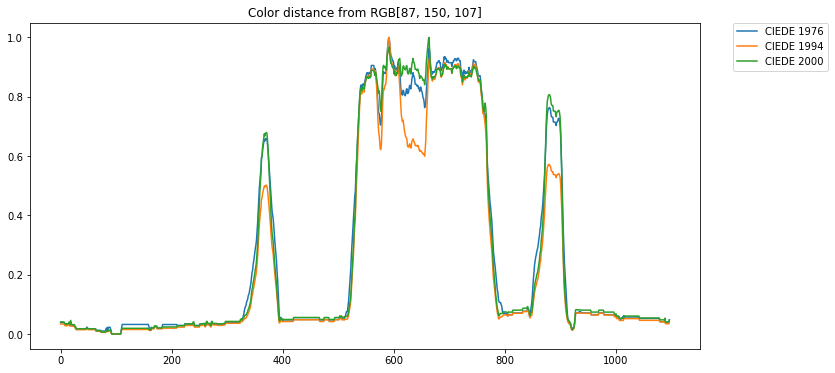
\includegraphics[width=\textwidth]{gfx/distances/ciede-comp.png}
		\caption{Comparison with different CIEDE $\Delta E$ variants}
	\end{subfigure}
\end{figure}
Additionally, CIEDE76 shows less variance on similar colored spaces to the 
target color as well as high color difference peaks on all other pixels. This 
yields an accurate upper and lower limit, in which the green screen can be 
calibrated in.
\newline
Finally, comparing CIEDE76, CIEDE94 and CIEDE2000 reveals, that CIEDE76 
performs well enough while having the lowest performance overhead. The 
similarities between the 1976 and 2000 method are very apparent, while 
CIEDE2000 has a significantly more complex algorithm. (cf.  
\cite{sharma:ciede2000:2005}) Performing the same operation on the same data 
with different CIEDE color distance revisions (fig. 
\ref{fig:chroma:image_comparison}e), that there is little difference between 
CIEDE76 and CIEDE2000.        % Chroma Key Section
\section{Camera Offsets}

\begin{lstlisting}
	> Is this text?
	< No, this is doge.
\end{lstlisting}      % Render Buffer Swapper
% !TeX spellcheck = en_US
% !TEX root = ../thesis-example.tex
%
\section{Mitigating Frame Jitter}

An additional step that can be handled by the same algorithm is the mitigation 
of frame or time jittering, a term that describes a effect of different running 
framerates of an actors captured video footage and rate of 3D environment 
rendering. Since the native framerate of the HMD is higher than the frames 
produced by the video feed, there will be noticeable small jitters of virtual 
camera movement, which are not present on the source video material. The HTC 
Vive Controller are very good at picking up minuscule changes in motion, which 
are instantly translated to the transform of the camera rig and then result in 
minor motion of the 3D environment. Visually this shows in a shaking virtual 
world while the real world video stands still.
\newline
To minimize the effect, it is possible to overwrite framebuffers for as long as 
one duration of a video frame and then swapping out these buffers. The headset 
recommends to run it at 90fps - miss timings are no issue either, since it 
results in non noticeable errors in virtual projections while the displayed 
frame is stable visual performance is unaffected. Thus it is possible to write 
less than three times into a framebuffer, which is mitigated again by 
displaying the final result later - the final image is therefore unaffected 
besides imperceptible differences between the real world camera and its virtual 
position.

\todo[inline]{needs then lstlisting when the code further up is modified}
			  % Frame Jitter Mitigation
% !TeX spellcheck = en_US
% !TEX root = ../thesis-example.tex
%
\section{Virtual projection parameters from real world camera}
\label{sec:projection-params}
To produce a virtual projection there are four unknowns to solve for:

\begin{my_list}
	\item Position of the real world camera
	\item Rotation of the real world camera
	\item Field of View (FoV) of the camera
	\item Distance between the HMD and the real world camera
\end{my_list}

Luckily the former two are solved by the tracking solution, thus can be used 
directly as transformation matrix for the virtual camera - ignoring an 
additional offset from the actual controller to the camera, which is accounted 
for inside the software.
\newline
The calculation of a corresponding distance between a camera and the Vive HMD 
to control the virtual projection parameters can be solved, too: Since both 
devices are tracked, one natively and the other with a controller as 
tracking anchor, it can be calculated with the same euclidean distance as 
discussed earlier, with $C$ as camera position and $H$ as HMD position:

\eq{eq:zsort:distance}{
	Z = \sqrt{(C_X + H_X)^2 + (C_Y + H_Y)^2 + (C_Z + H_Z)^2}
}

\begin{figure}[htb]
	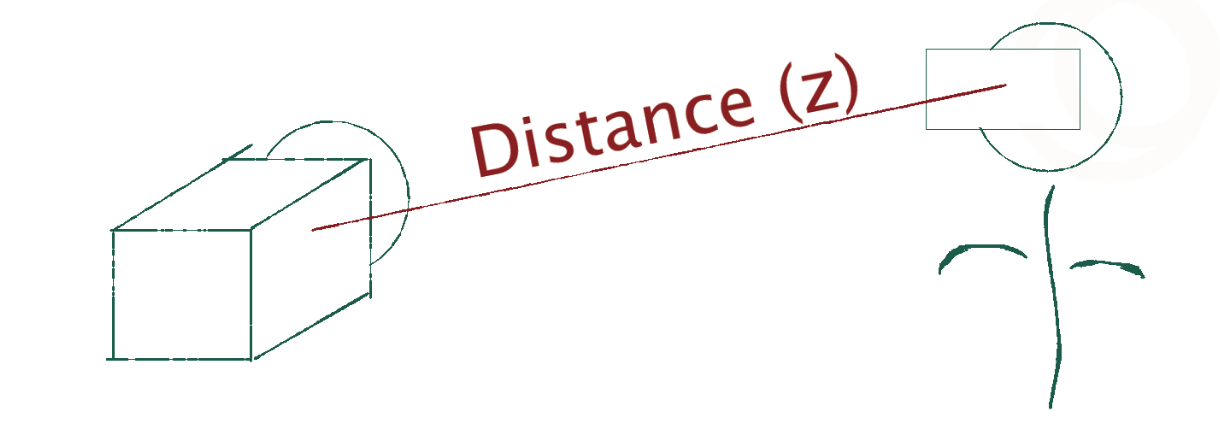
\includegraphics[width=\textwidth]{_raw_resources/composition/Composition-Z-Distance.png}
	\caption{Distance correlation}
	\label{fig:projection:distance}
\end{figure}

Another important projection parameter is field of view. Most production 
cameras only declare a focal length on lenses - which makes sense in that 
context, since field of view is a constraint between sensor size and focal 
length. Through the specification sheet of the camera the current field of view 
can be calculated inside Unity, with the sensor height as $S_h = 17.3mm$ and 
focal length as $F_l = 14mm$:

\eq{eq:zsort:fov}{
	FoV = 2*tan^{-1}\frac{S_h}{2 * F_l}
}

\eq{eq:zsort:fov:result}{
	FoV = 63.42028^\circ
}

With that we have now all projection parameters for the virtual environment to 
generate an image that matches in relative transformation parameters as the 
real world camera would look at. % Projection Parameters
% !TEX root = ../thesis-example.tex
%
\section{Virtual Z Sorting}

\todo[inline]{here a recap image of current steps: keying + delaying}

We have now a properly keyed video feed and synchronous motion between the VR 
actor and the 3D environment. To increase the immersion of that composition the 
next important step is to sort the scene on a tri-graph of planes.

\begin{figure}[htb]
	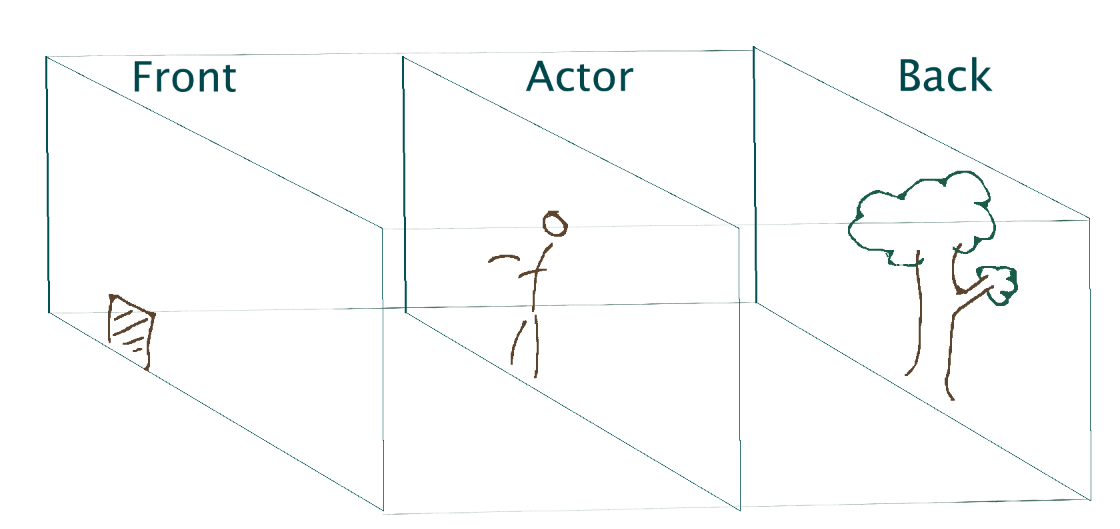
\includegraphics[width=\textwidth]{_raw_resources/composition/Composition-TriGraph.png}
	\caption{A sketch of the video composition with three layers of projection}
	\label{fig:zsort:sketch}
\end{figure}

There are multiple ways to achieve proper segmentation and composition of all 
three layers, depending on the rendering method. Deferred shading allows for 
better lightning simulation in engine but changes alpha- and depthmaps of a 
rendered scenery - this yields incorrect layer blending and results into an 
incorrectly displayed image. This software takes account for this and lets 
creators decide between two render modes:

\begin{my_list}
	\item Replace Masking: A front plane is displayed, after it follow the 
	chroma-keyed video and then the background. This is the most accurate image 
	generation.
	\item Alpha Masking: A front alpha mask of the geometry is displayed, then 
	the actor is mixed with a full render image of the background. The 
	resulting image has inconsistencies with alpha-blending but this method 
	works with all rendering setups.
\end{my_list}

The decision is between accuracy and presentation. Many post processing effects 
or deferred shading are not able - or simply do not respect - the alpha matte, 
which is usually no issue, since these steps are taken after rendering is 
complete, thus causing no unwanted side-effects. Other post effects need 
certain projection requirements and / or get disregarded through culling, like 
in Figure \ref{fig:zsort:comparison:front} where the volumetric lightning is 
culled out of the virtual projection and therefore gets completely ignored, 
resulting in a black front geometry.

\begin{figure}[htbp]
	\caption{A comparison of different composition methods in engine}
	\label{fig:zsort:comparison}
	\begin{subfigure}[t]{.45\textwidth}
		\centering
		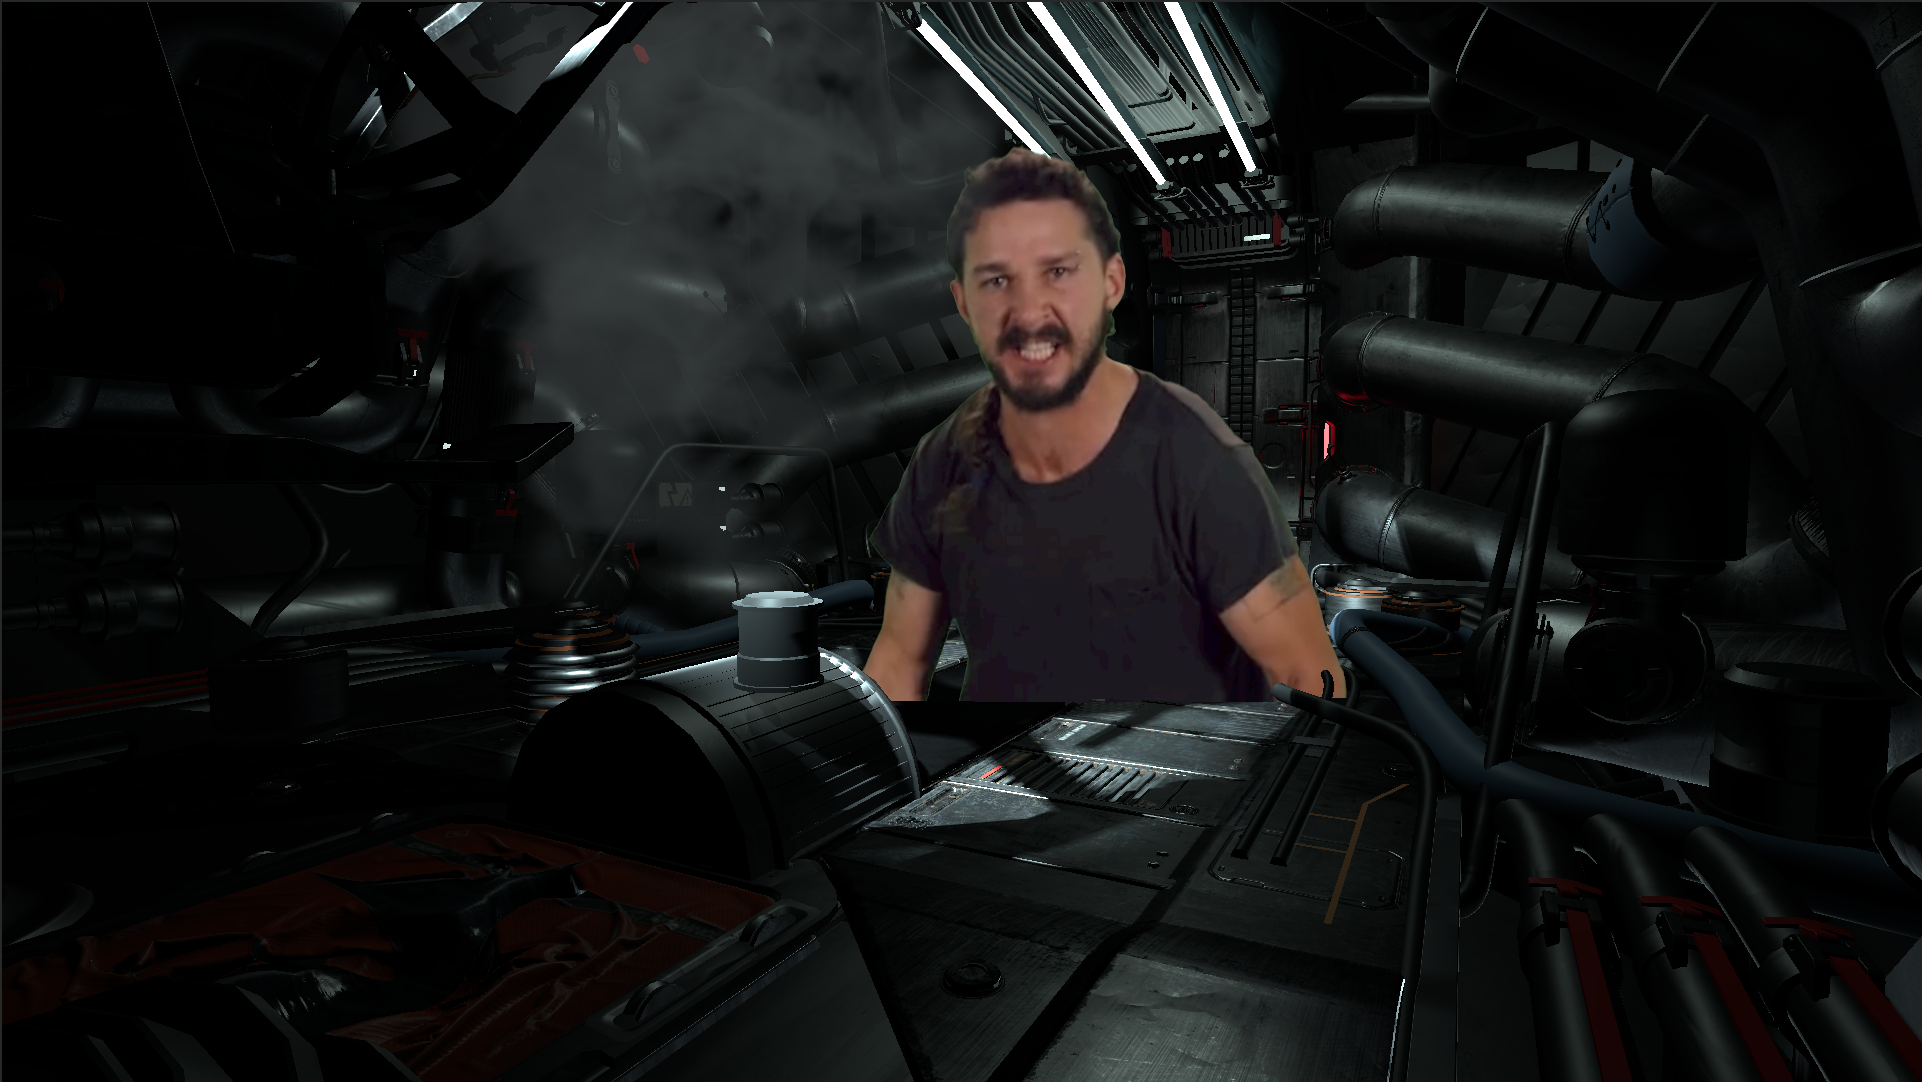
\includegraphics[width=\textwidth]{_raw_resources/composition/Composition-Perfect-Realigned.png}
		\caption{The proposed composition, simulated, with an arbitrary depth 
		of the video feed}
	\end{subfigure}
	\begin{subfigure}[t]{.45\textwidth}
		\centering
		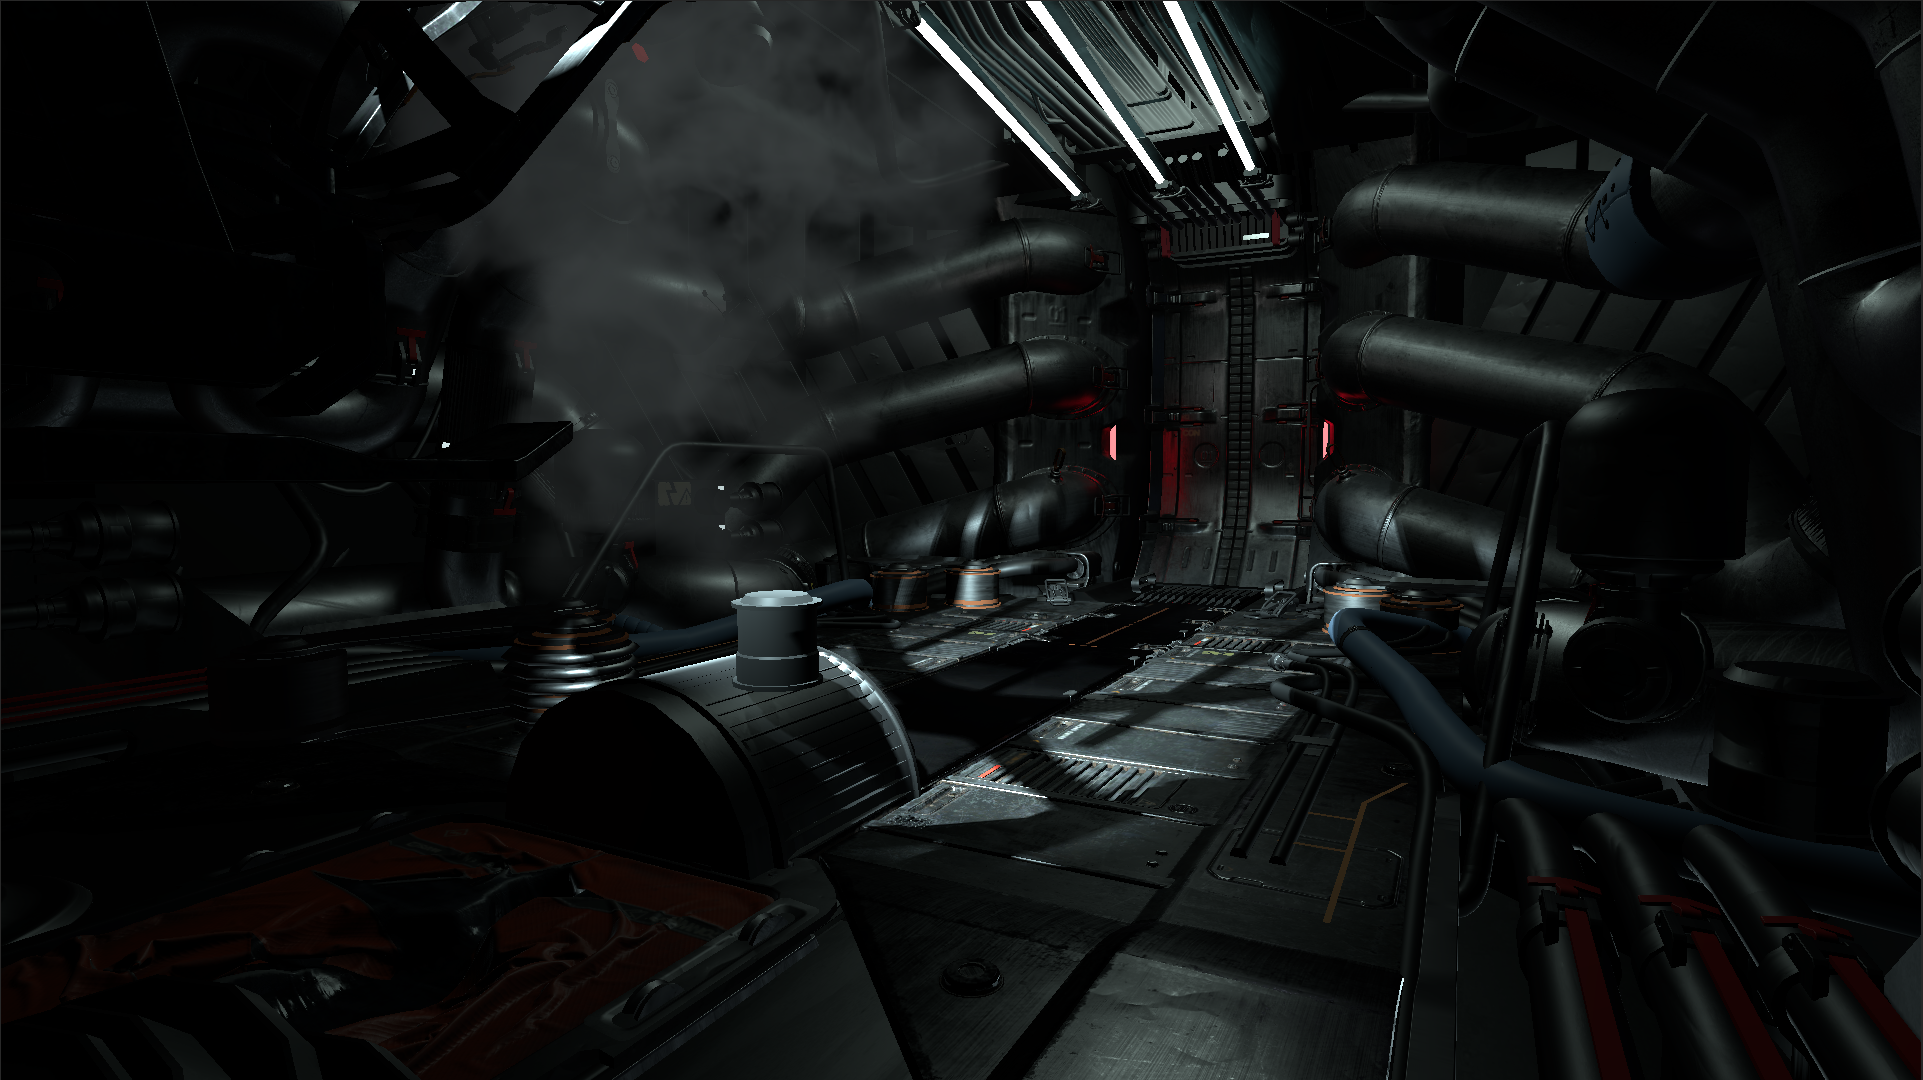
\includegraphics[width=\textwidth]{_raw_resources/composition/Composition-Full-Render.png}
		\caption{The full length rendering}
	\end{subfigure}
	\newline
	\begin{subfigure}[t]{.45\textwidth}
		\centering
		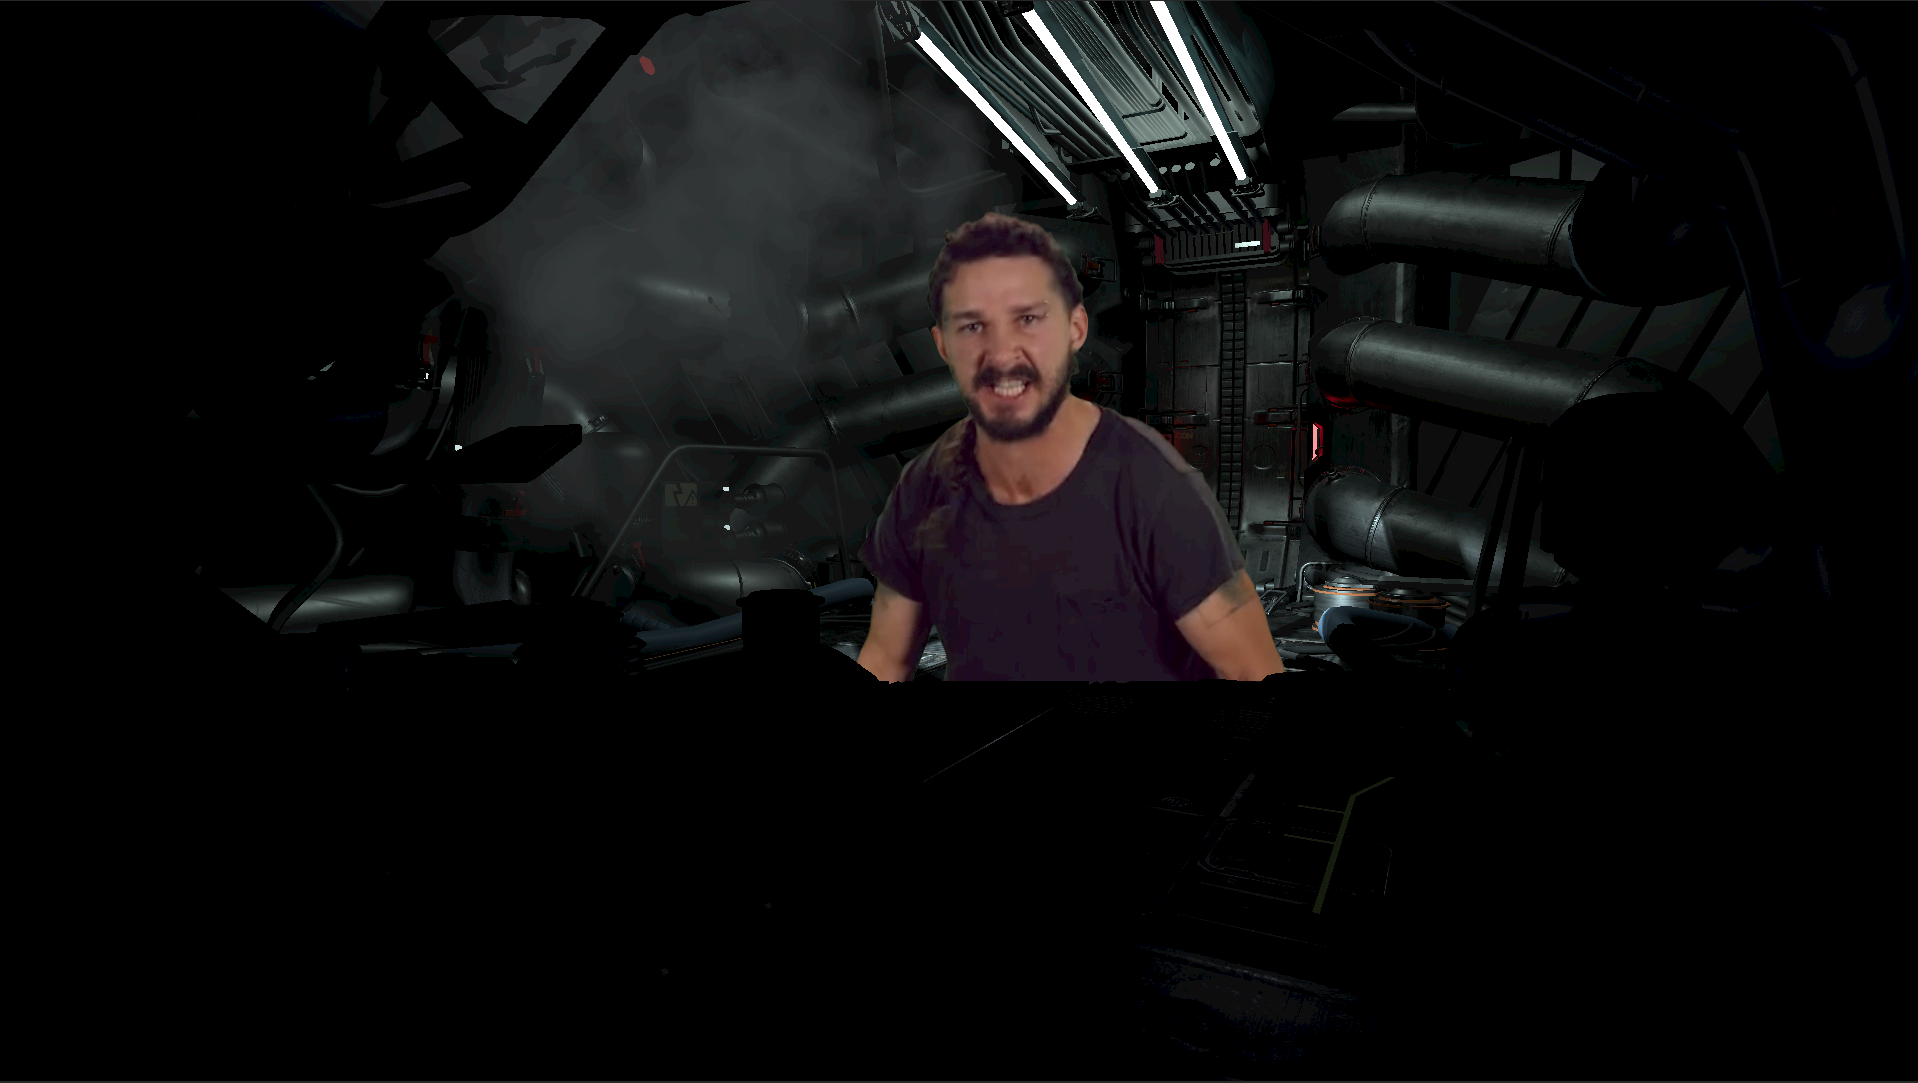
\includegraphics[width=\textwidth]{_raw_resources/composition/Composition-Front-Replace_orso.png}
		\caption{A composition by rendering a front, followed by the video and 
		then the background}
	\end{subfigure}
	\begin{subfigure}[t]{.45\textwidth}
		\centering
		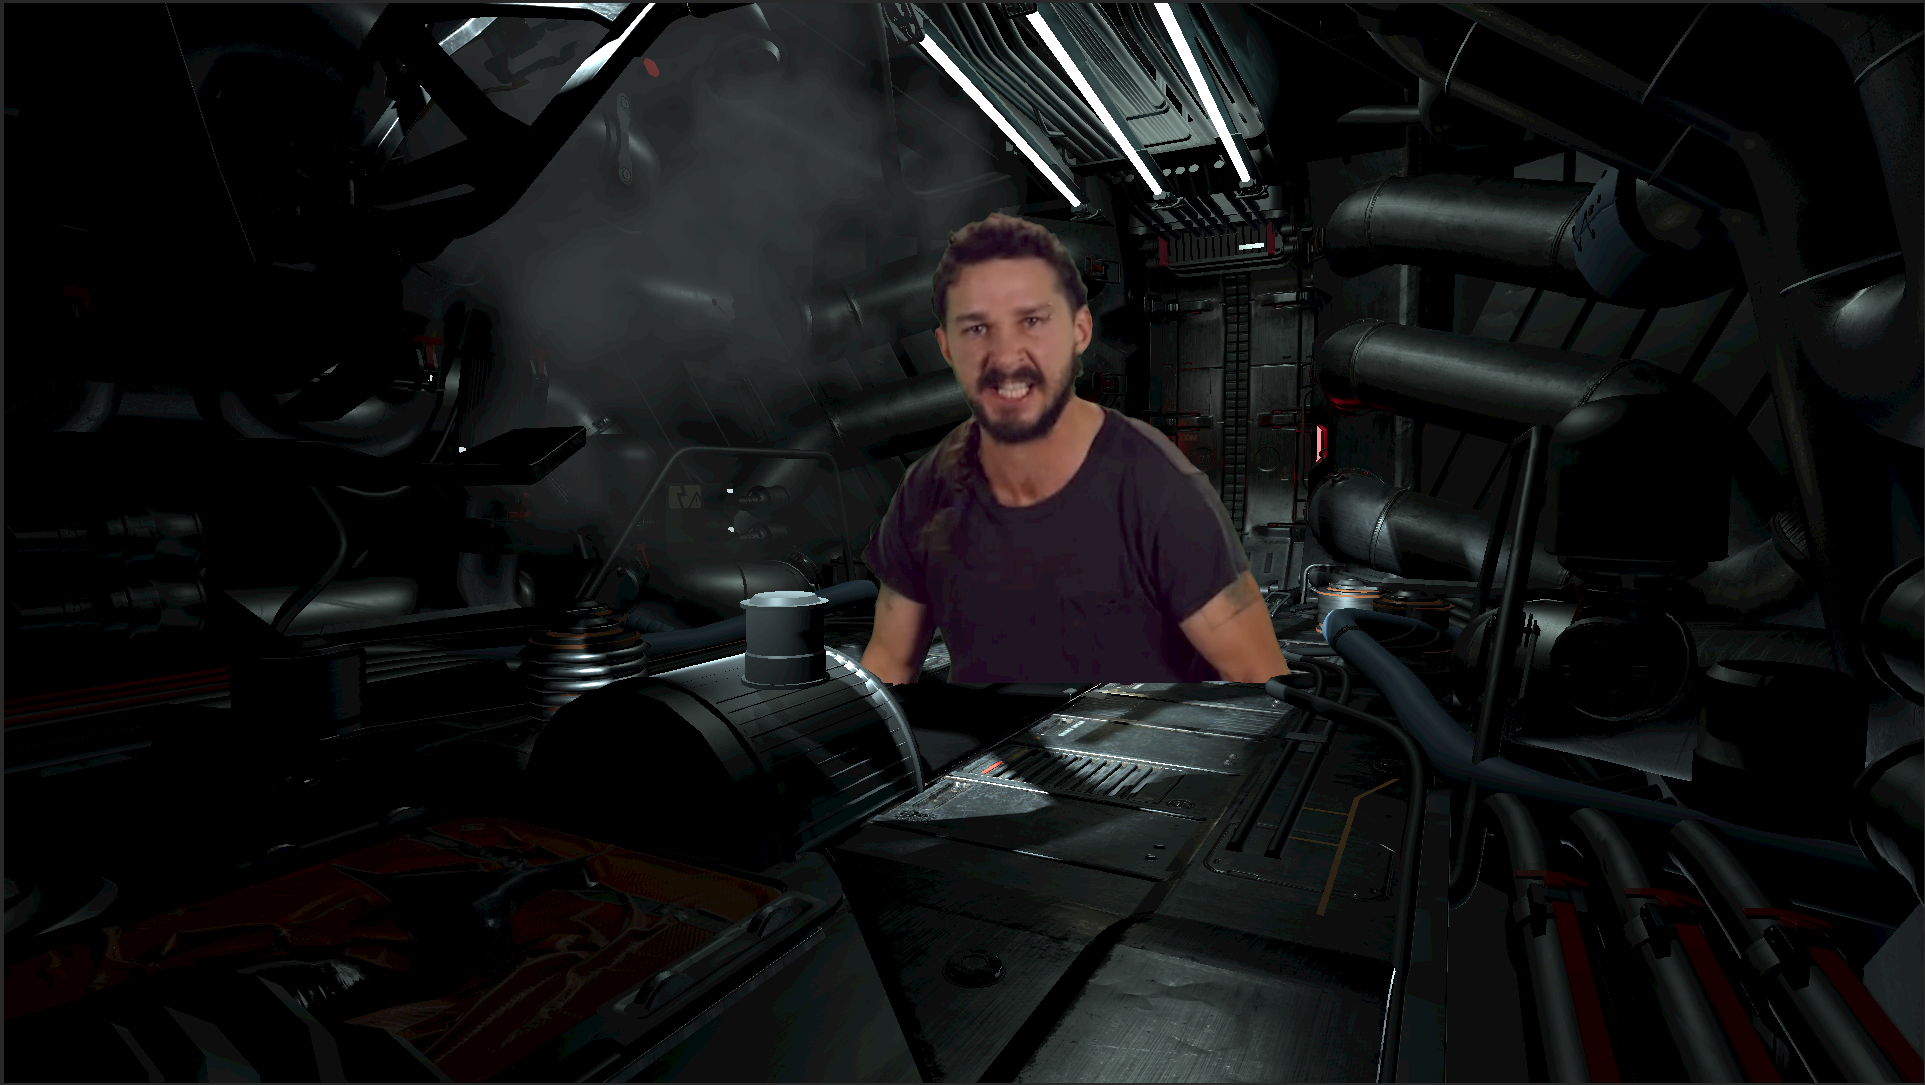
\includegraphics[width=\textwidth]{_raw_resources/composition/Composition-Front-Mask.png}
		\caption{A composition with the front geometry as mask, and then a 
		mixing of the video and a full length render}
	\end{subfigure}
	\newline
	\begin{subfigure}[t]{.45\textwidth}
		\centering
		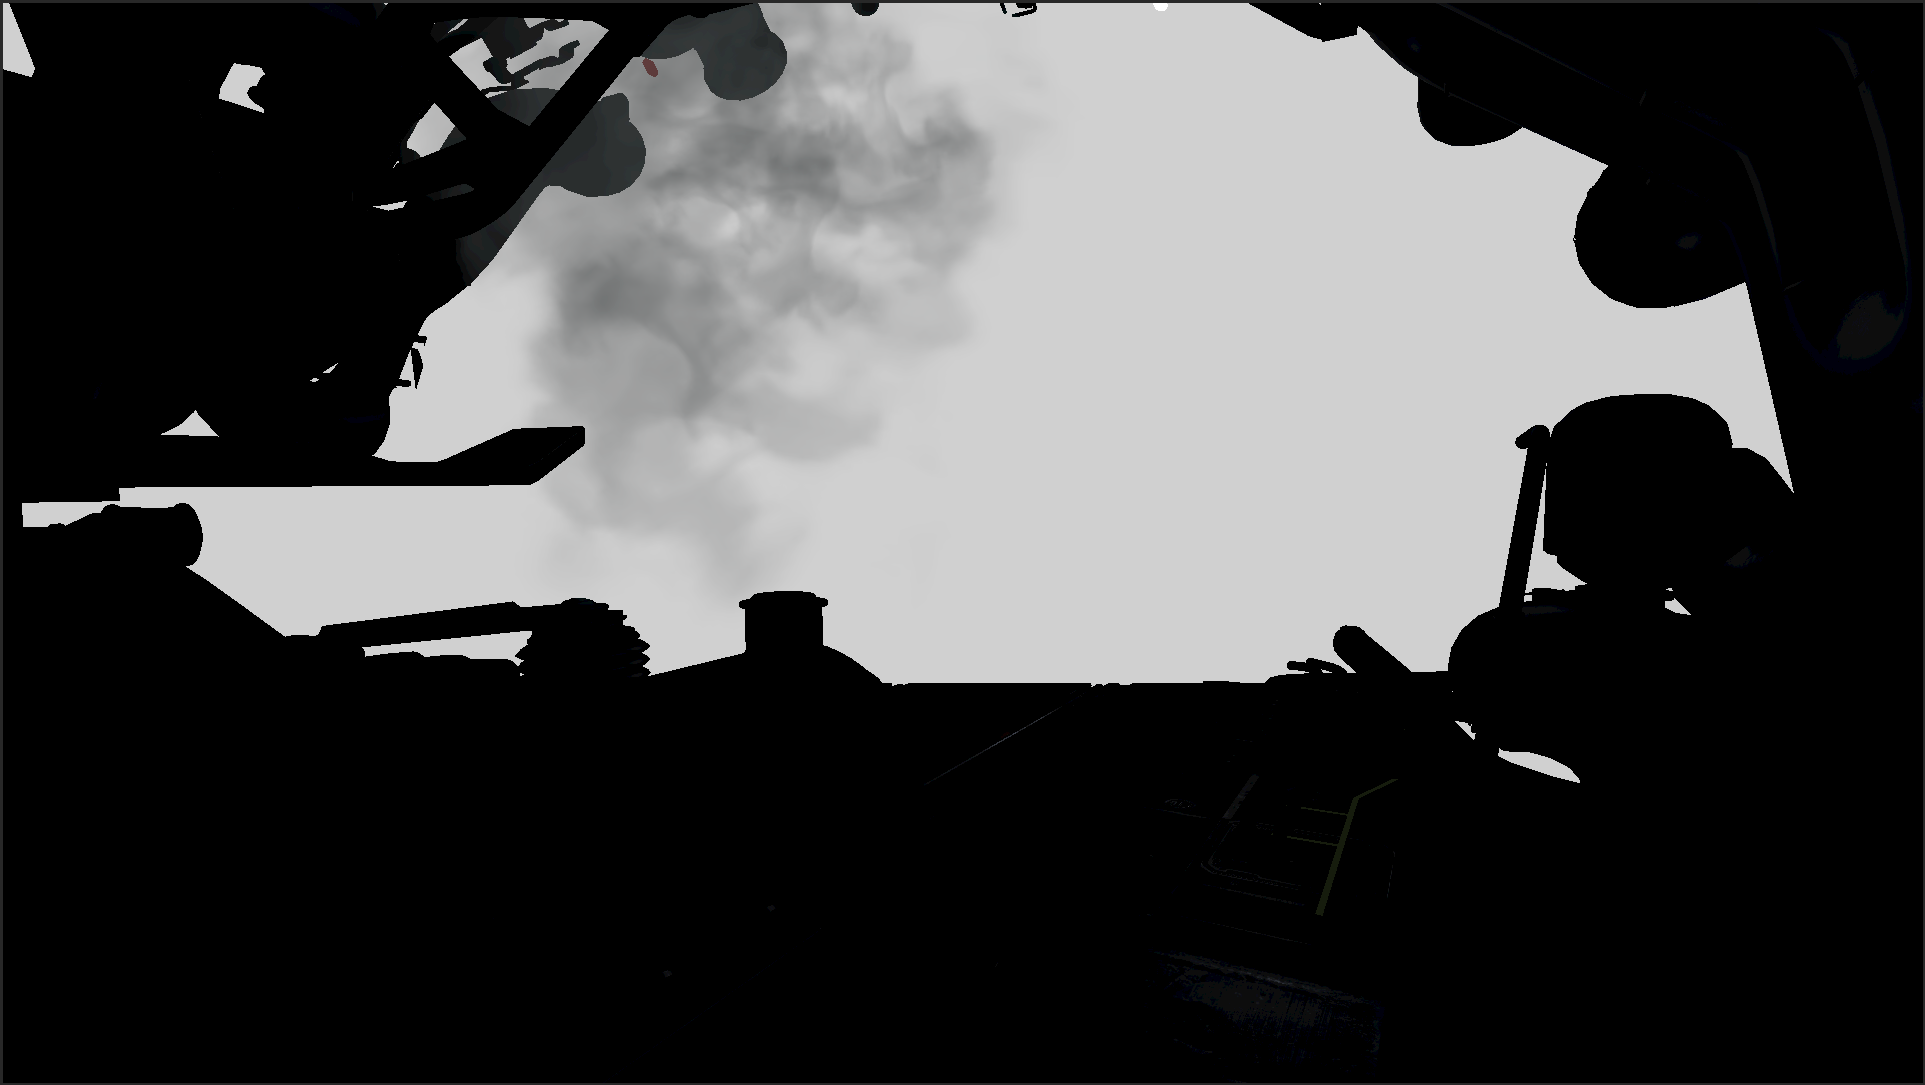
\includegraphics[width=\textwidth]{_raw_resources/composition/Composition-Front.png}
		\caption{The virtual projection of the front camera - volumetric 
		lightning does not work due to the short projection length}
		\label{fig:zsort:comparison:front}
	\end{subfigure}
	\begin{subfigure}[t]{.45\textwidth}
		\centering
		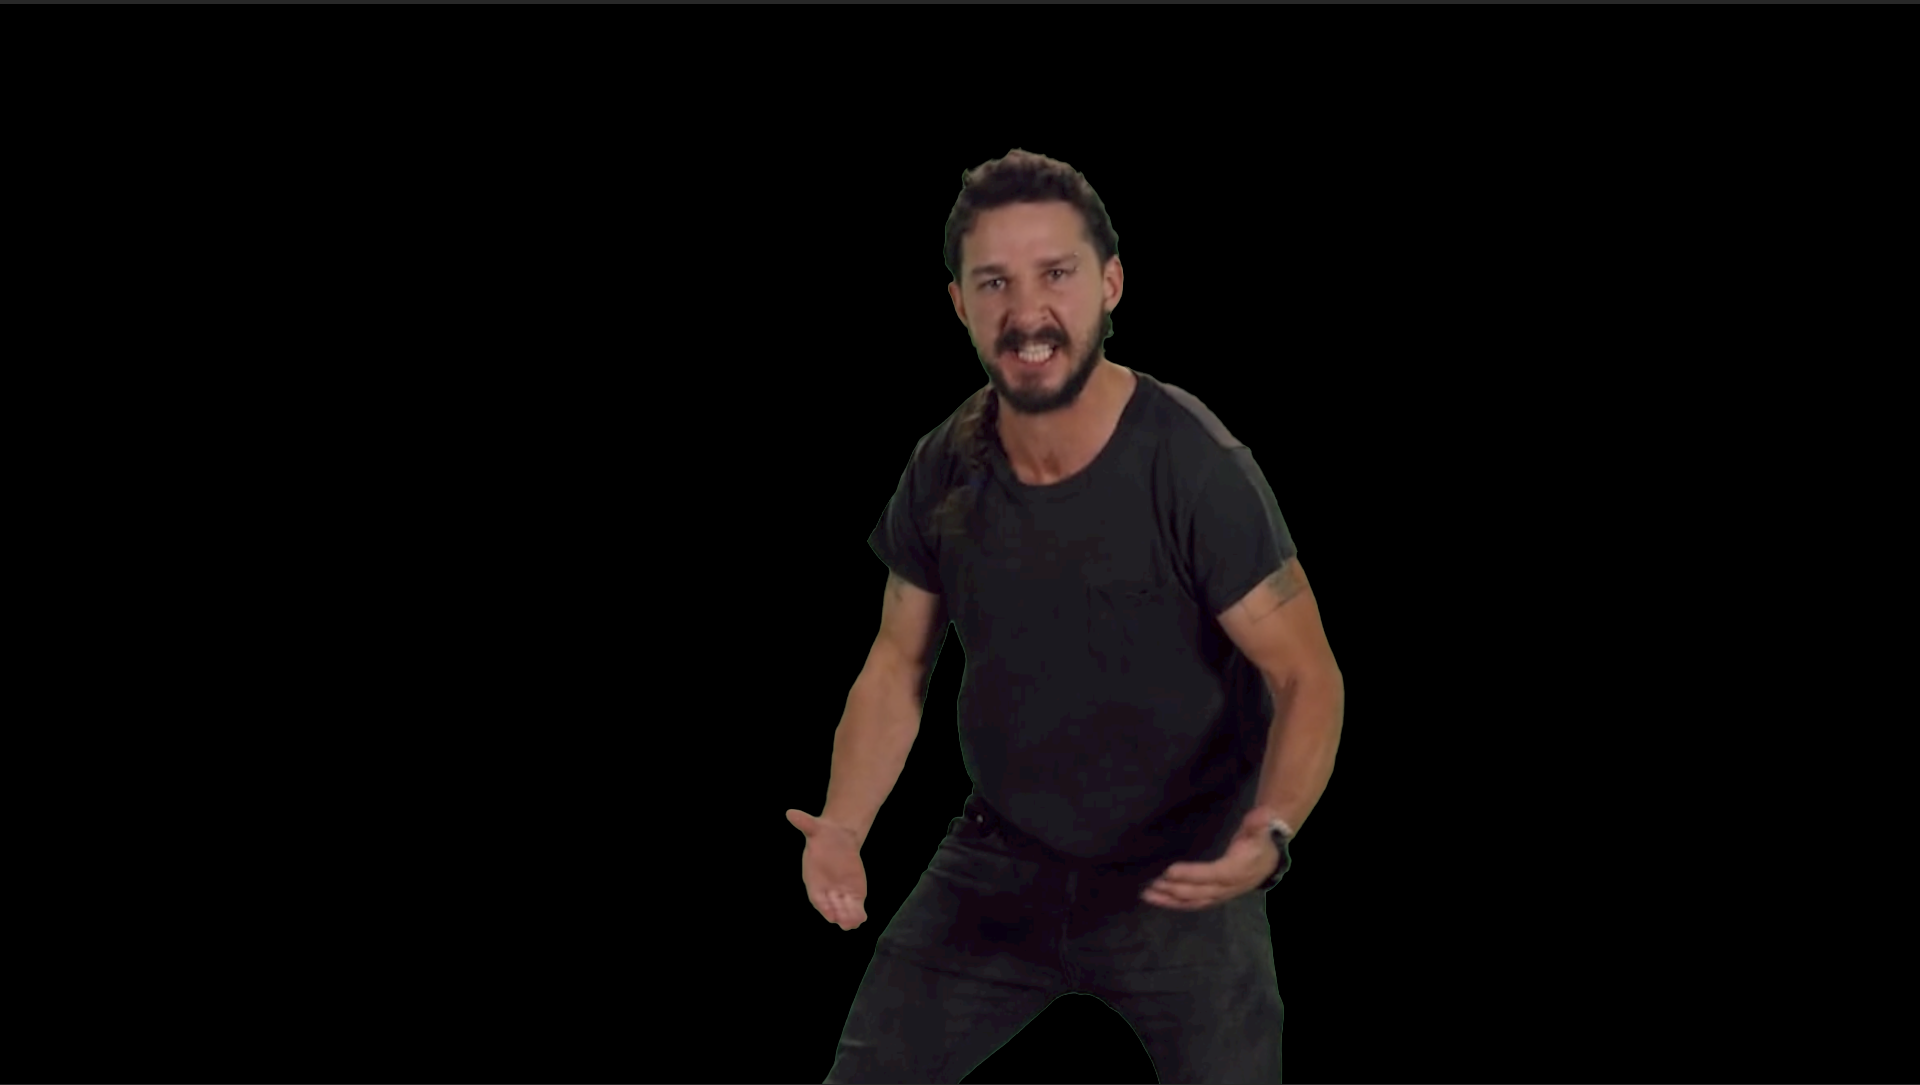
\includegraphics[width=\textwidth]{_raw_resources/composition/Composition-Chroma-Result.png}
		\caption{The chroma keying result}
	\end{subfigure}
\end{figure}

Mixing these three layers are similarly easy, using a previous equation 
\eqref{eq:chroma:assumption:alpha:weak} and 
\eqref{eq:chroma:assumption:alpha:cont}. Assuming an ARGB front render image 
$F$, a RGB video feed  $V$ and the RGB background $B$, 
we can mix all three layers effortlessly:

Replace Masking:

\eq{eq:zsort:replmask:1}{
	\alpha_T = \alpha_V * (1 - \alpha_F)
}


\eq{eq:zsort:replmask:2}{
	I(x, y) = (1 - \alpha_T) * F(x, y) + \alpha_T * V(x, y)
}

\eq{eq:zsort:replmask:3}{
	\alpha_S = \alpha_B * (1 - \alpha_{I(x, y)})
}


\eq{eq:zsort:replmask:4}{
	J(x, y) = (1 - \alpha_S) * I(x, y) + \alpha_S * B(x, y)
}

Alpha Masking is very similar with transforming the alpha-mask of the webcam 
footage after chroma-keying it. It is masking the video further, after the 
video matte is pulled already:

\eq{eq:zsort:alphamask:1}{
	\alpha_{V_T} = 
	\begin{cases}
		1 - \alpha_F  & \quad \text{if } \alpha_V > 0 \\
		\alpha_V      & \quad \text{otherwise}
	\end{cases}	
}

\todo[inline]{This is a bit incorrect as what is currently used in the shader.}

\eq{eq:zsort:alphamask:2}{
	\alpha_T =  \alpha_B * (1 - \alpha_{V_T})
}

\eq{eq:zsort:alphamask:3}{
	I(x, y) = (1 - \alpha_T) * V(x, y) + \alpha_T * B(x, y)
}

\todo[inline]{remindme: there is the depth-offset missing currently.}

Now we have a well mixed image composition where the actor is placed in between 
two projections and thus can have an interactive fore- and background. The 
initial assumption is, that the actors depth is flattened, based on the 
distance between a real world camera and the Vive Head Mounted Display.
    % Camera Z Sort
% !TeX spellcheck = en_US
% !TEX root = ../thesis-example.tex
%
\section{Additional Camera Stencil}

When producing on small and / or amateur sets, there are usually constraints to 
size and proportions of the greenscreen production, thus limiting the 
record-able space. Since a calibrated play space can be fetched from the 
SteamVR API to receive a proper-sized bounding box, it is possible to do a 
projection of the greenscreens real size inside a virtual scene and use this as 
a stencil for the incoming video feed, effectively cropping off around all 
edges outside of a calibrated greenscreen. Effectively this means that a real 
world camera can film outside the edges of a green screen and it will not 
degrade the visual performance of the image composition.

\begin{figure}[htb]
	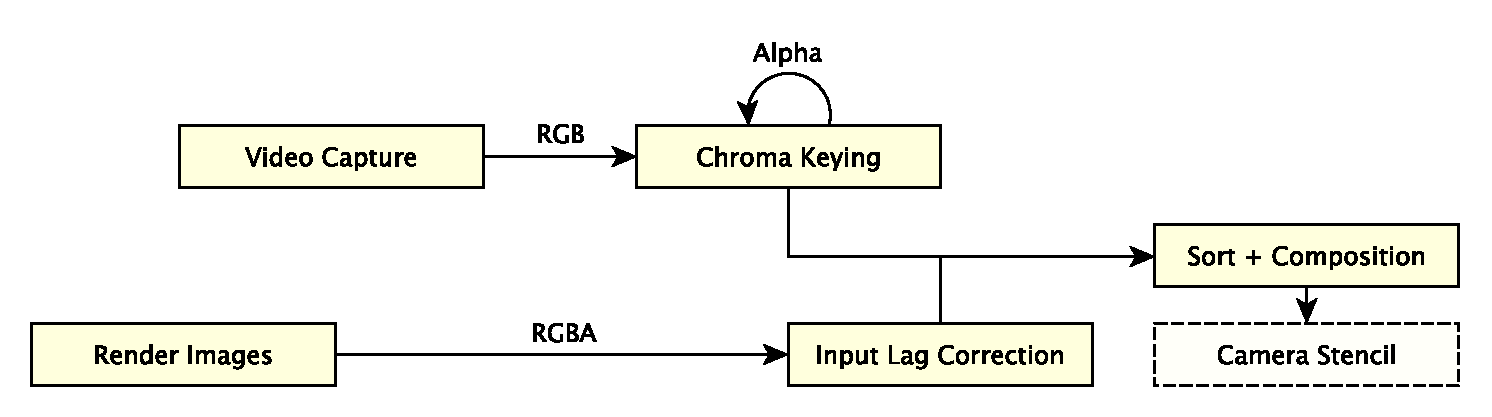
\includegraphics[width=\textwidth]{_raw_resources/pipeline_steps/4_6_stencil.pdf}
	\caption{After sorting the scene additional stenciling is necessary}
	\label{fig:steps:stencil}
\end{figure}

A virtual projection can be seen in figure \ref{fig:stencil:projection} with 
reconstructed camera parameters. With help of the engine-editor a greenscreen 
can be calibrated and should match very closely to all real world parameters, 
allowing a real world camera to film over the edges of a greenscreen without 
destroying the image composition. If a VR actor is outside of the chroma key 
planes, the resulting image composition wouldn't be usable, thus this solution 
enhances a resulting image without major drawbacks.

\begin{figure}[htbp]
	\caption{Virtual projection and photo of VR actor - note: in-engine 
	screenshot and photos were taken shortly apart and therefore don't fit 
	exactly}
	\label{fig:stencil:projection}
	\begin{subfigure}[t]{.45\textwidth}
		\centering
		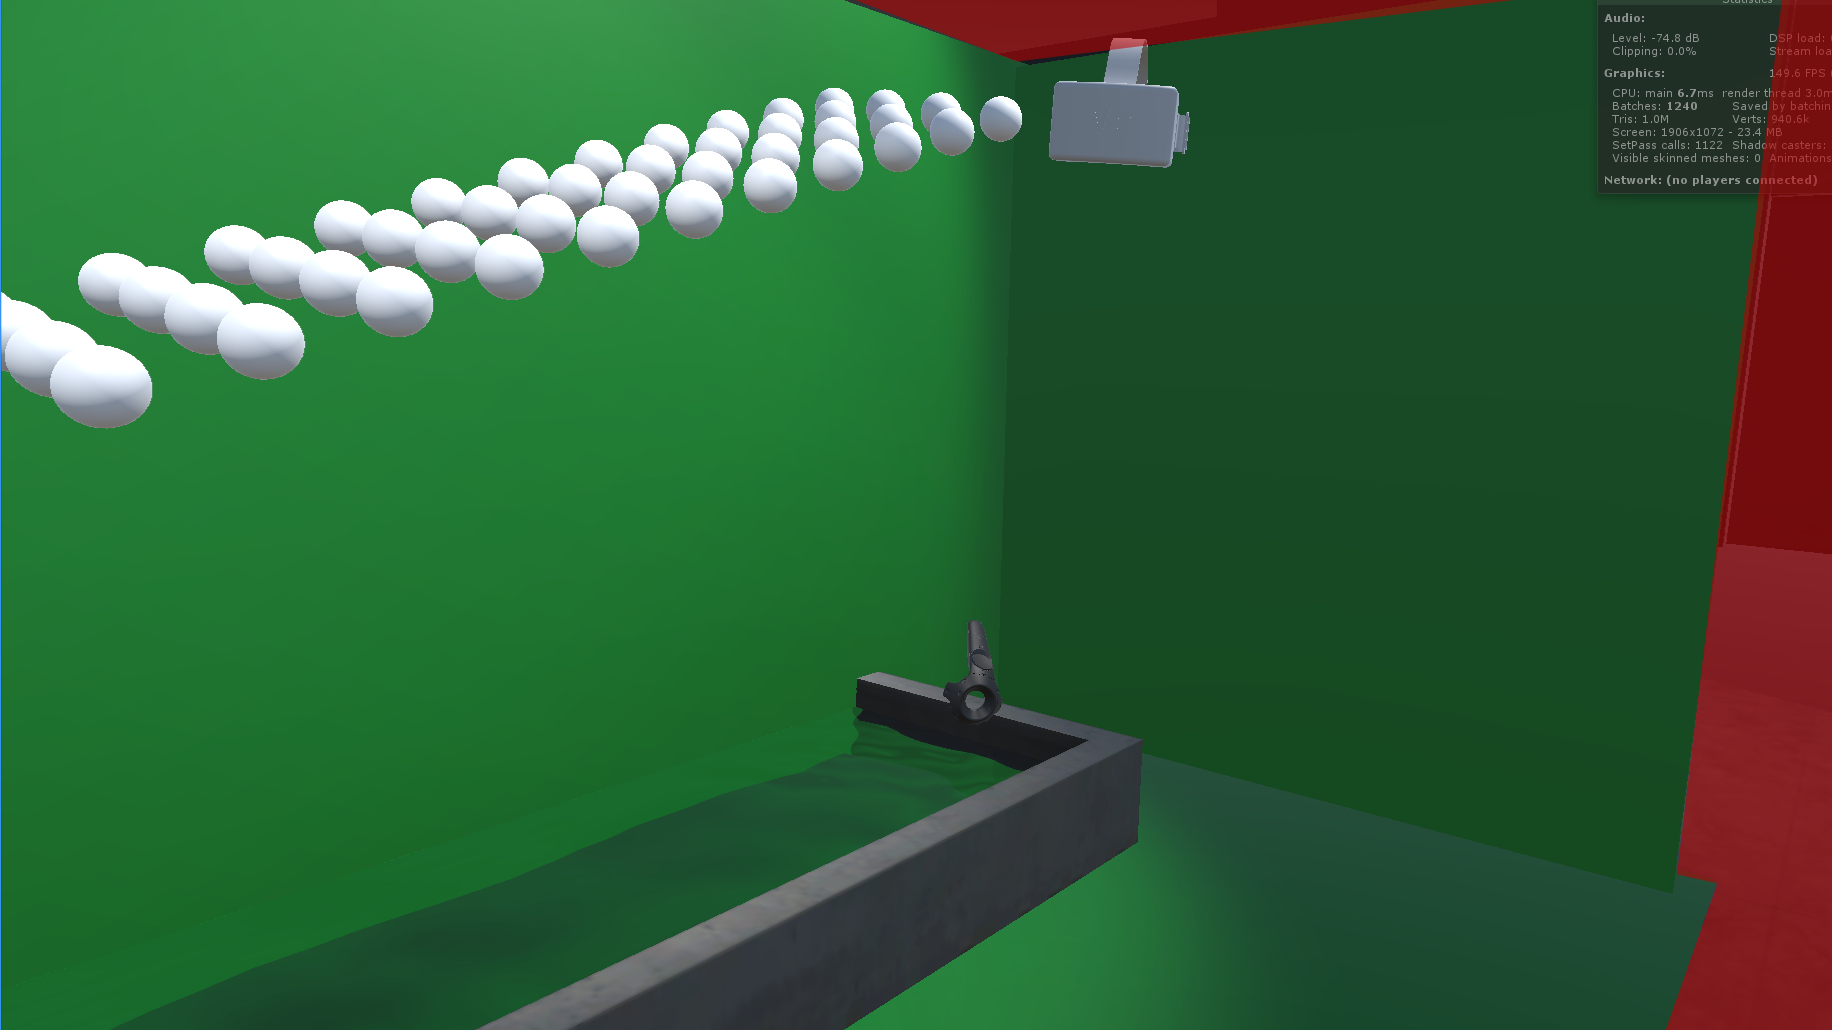
\includegraphics[width=\textwidth]{gfx/StencilProjection.png}
		\caption{Virtual reprojection of valid green screen - red colored areas 
		will be cut off}
	\end{subfigure}
	\begin{subfigure}[t]{.45\textwidth}
		\centering
		\includegraphics[width=\textwidth]{gfx/StencilCut.png}
		\caption{Masking what would be remaining video content - red colored 
		areas will be cut off}
	\end{subfigure}
\end{figure}

In-engine this setup is a simple addition: After registering another camera to 
the camera manager, it simply renders a green box. Taken from previous 
projection parameters in \ref{sec:projection-params} this virtual camera 
receives a dedicated culling mask which only contain all green box projection 
planes. All other cameras ignore this layer. After each drawn frame, Unity is 
able to clear the framebuffer with a color alpha as 0 - all remaining fragments 
from the green box write any color with an alpha as 1. This creates a lookup 
texture where an alpha-mask is created which will be transferred to the video 
feeds alpha.

Now we achieved a green box projection inside the same scene without using 
complex management processes with Unitys' scene manager. Due to the quick setup 
it works well for fast calibration and allows for a broad camera angle without 
degrading the mixed reality performance.
\newline
Unfortunately stencil-opertions are poorly documented in Unity and add an 
overhead which cannot be measured from builtin profiler tools - as such it adds 
unknown performance costs and have not been used in this thesis.		  % additional camera masking
% !TeX spellcheck = en_US
% !TEX root = ../thesis-example.tex
%
\section{Light Environment Reproduction}

To conclude all rendering steps taken by now: We have successfully created an 
image composition with correct projection parameters, recalculated a planar 
depth, synchronized in-engine frames with the camera input lag and realigned 
the frame rate between both image generating systems and cut off all overshot 
pixels that were recorded outside of the green screen.

\begin{figure}[htb]
	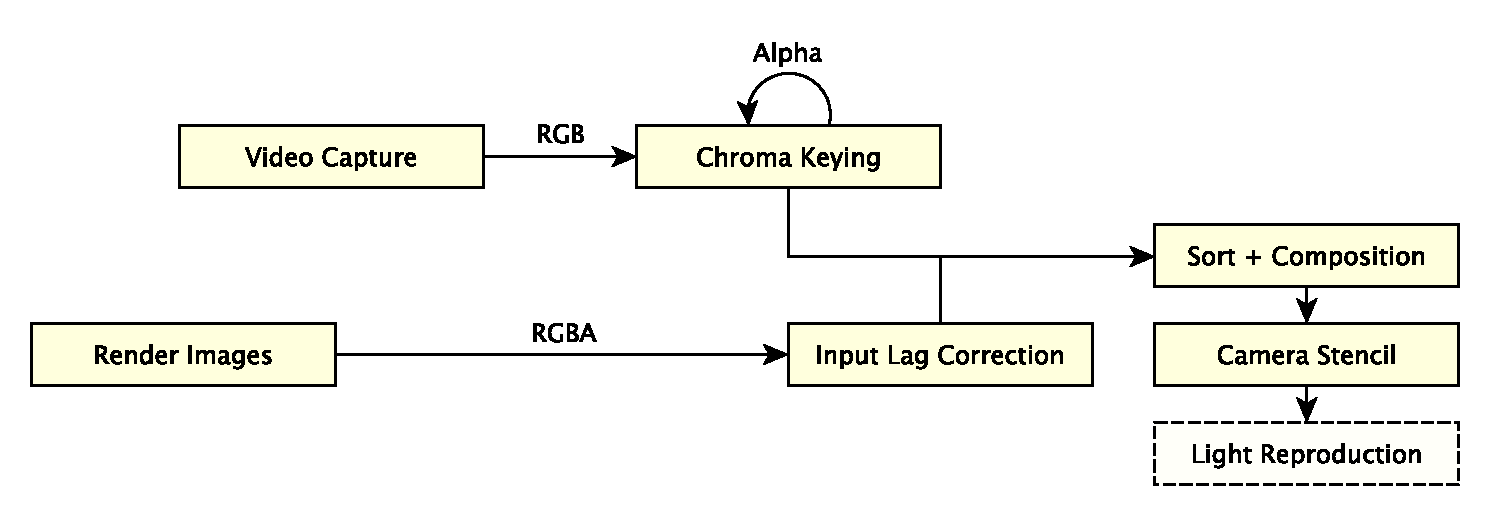
\includegraphics[width=\textwidth]{_raw_resources/pipeline_steps/4_7_lights.pdf}
	\caption{Following in this pipeline is lights reproduction}
	\label{fig:steps:lights}
\end{figure}

A minor last step is light-reproduction, in which an approximate lightning 
setting will be transferred from 3D environment to the video feed of a VR 
actor. Assuming that the video footage contains a natural lit, tint-free and 
calibrated video signal, it is possible to approximate how a VR actor would 
be lit like if he truly is inside the virtual environment.

\begin{figure}[htb]
	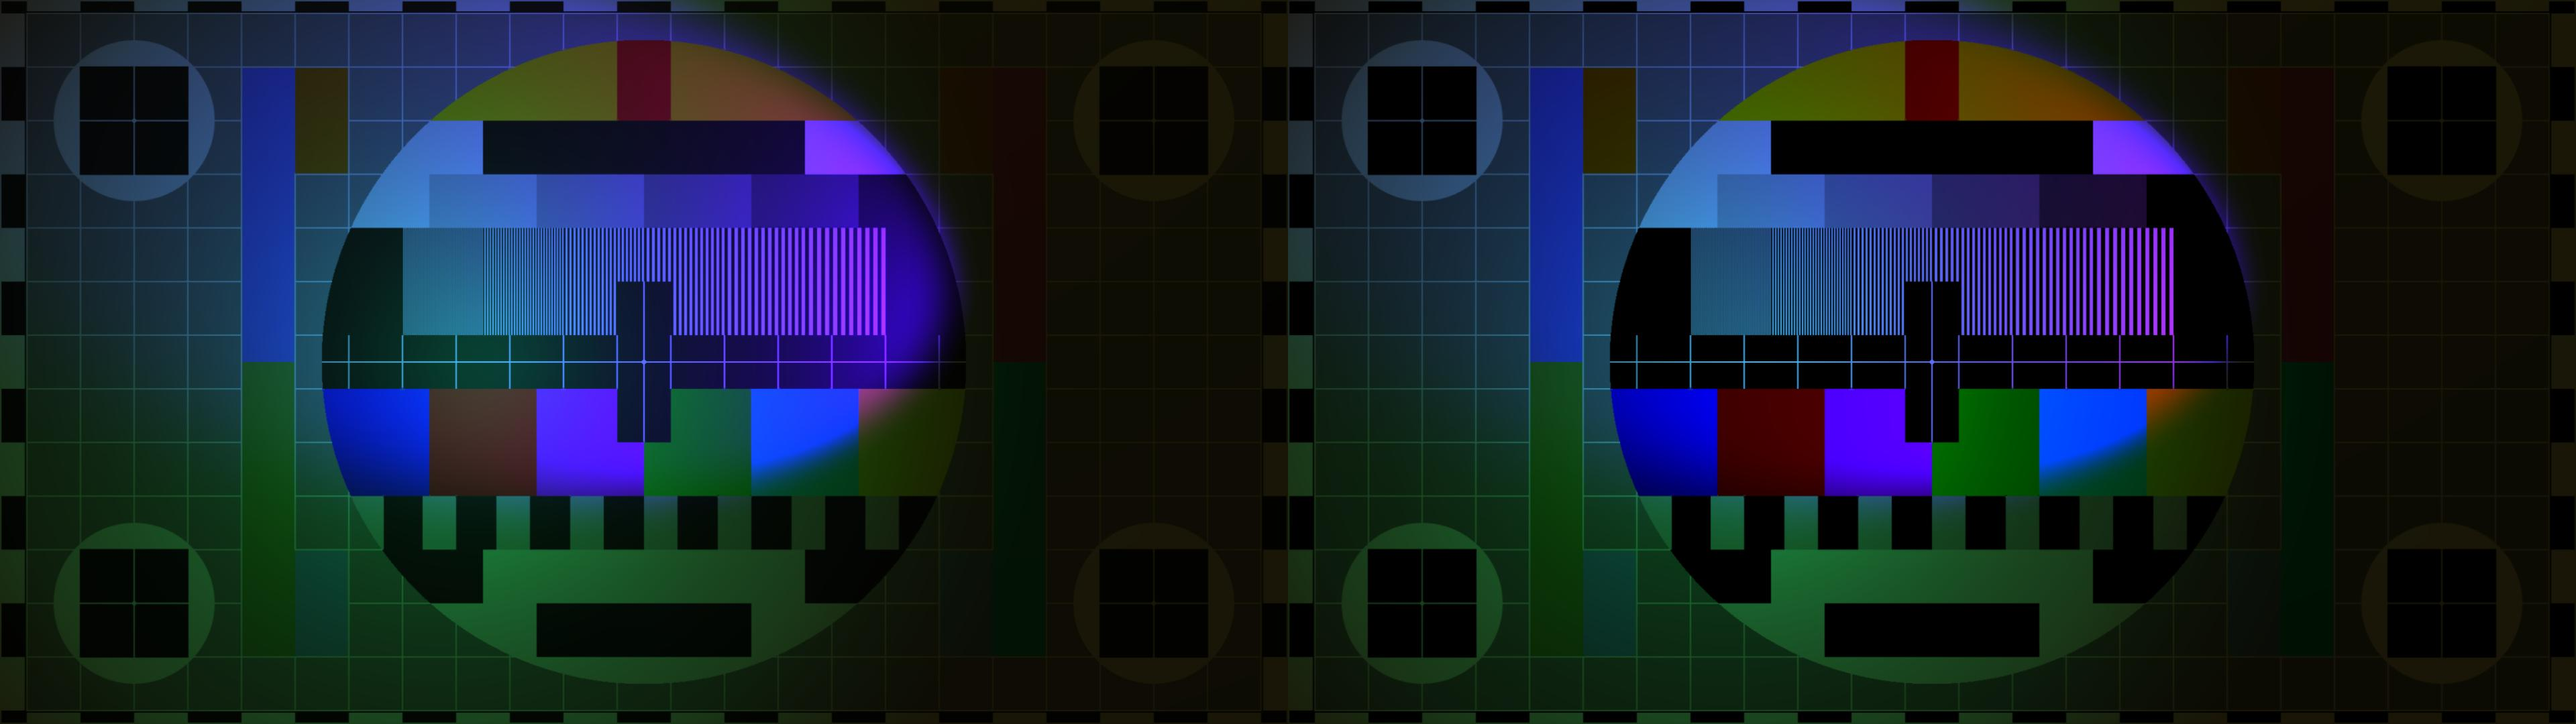
\includegraphics[width=\textwidth]{_raw_resources/light-reconstruction/comparison.jpg}
	\caption{Left: original, Right: reconstruction}
	\label{fig:light-reconstruction:comparison}
\end{figure}

Ambient light reproduction hinges on two assumptions: An actor's recorded video 
is flat for this purpose \textit{and} he receives clean and consistent light 
from all angles that has no additional glossiness. With that we can project a 
plane at the actor's position, filling the frustum edges of another virtual 
camera with the same camera projection parameters from section 
\ref{sec:projection-params}. This plane contains a simple lit material with 
white albedo coloring, which captures the lightning situation at this given 
point (figure \ref{fig:light-reconstruction:diff-capture} a).

To calculate the position $P_{pos}$ and size $\vec{P_{x, y}}$ with a 
given forward vector $\vec{C_{forward}}$ and position $C_{pos}$ of the 
camera, as well as a distance $Z$ between camera and actor and a current Field 
of View $FoV$ in radians by assuming a 16:9 video feed:

\eq{eq:light-reproduction:pos}{
	P_{pos} = C_{pos} + Z * \vec{C_{forward}}
}

\eq{eq:light-reproduction:size:1}{
	P_{x, y} =
	\begin{bmatrix}
		2 * \tan(FoV / 2) * Z \\
		P_{x} * \frac{16}{9}
	\end{bmatrix}	
}

These parameters can directly be applied to the transformation of said white 
plane which then captures the lightning environment inside the virtual scenes. 
As with all other composition-renderings, this step will be stored as a 
separate \code{RenderTexture} too and can operate on lower resolutions to speed 
up color and light sampling for performance gains.
\newline
The resulting frame buffer will be multiplied later onto the camera feed with a 
video color $C_V$ and the light plane $C_L$:

\eq{eq:light-reproduction:composition}{
	C_T = 
	\begin{bmatrix}
		C_{V_R} * C_{L_R} \\
		C_{V_G} * C_{L_G} \\
		C_{V_B} * C_{L_B}
	\end{bmatrix}
}

Lastly, a directional light with the same culling mask can be applied, to 
improve the overall brightness of this light mask to allow for more natural 
tint than a linear color operation.

\begin{figure}[htbp]
	\caption{A comparison of different composition methods in engine}
	\label{fig:light-reconstruction:diff-capture}
	\begin{subfigure}[t]{.45\textwidth}
		\centering
		
\includegraphics[width=\textwidth]{gfx/recoloring/plane.png}
		\caption{captured, lit plane}
	\end{subfigure}
	\begin{subfigure}[t]{.45\textwidth}
		\centering
		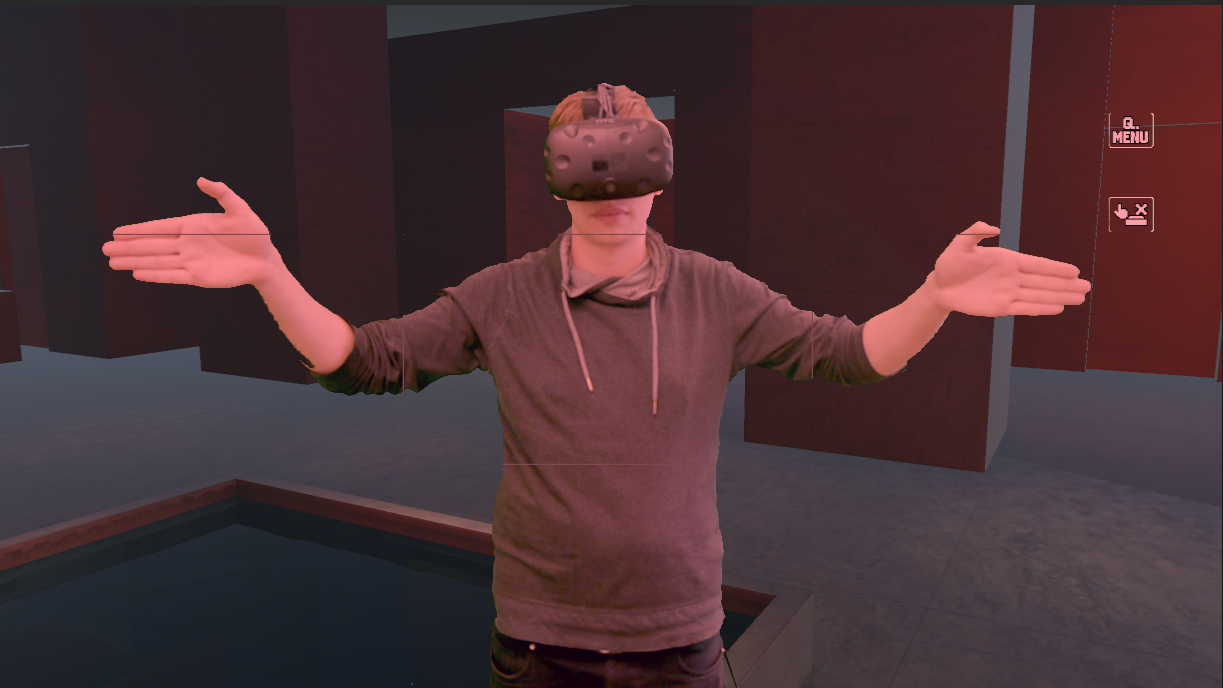
\includegraphics[width=\textwidth]{gfx/recoloring/img.png}
		\caption{Light plane applied to the actor}
	\end{subfigure}
\end{figure}

\todo[inline]{margin of error of light reproduction}
        % Light reproduction
% !TeX spellcheck = en_US
% !TEX root = ../thesis-example.tex
%
\section{Additional Coloring Operations}

Finally, we have created the best possible recreation of a VR actor inside the 
virtual reality scene. Now we can follow up with post effects on the video feed 
to fit it better into the environment.

\begin{figure}[htb]
	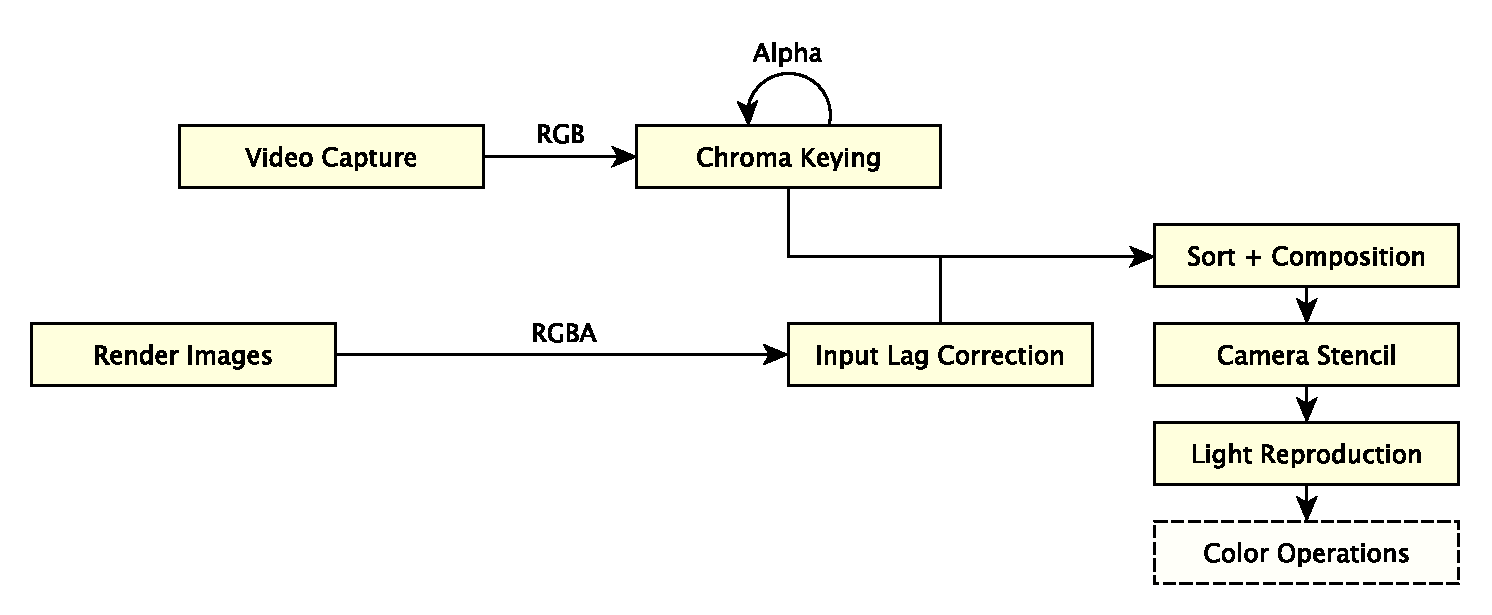
\includegraphics[width=\textwidth]{gfx/pipeline/4_8_color.pdf}
	\caption{Initial step upon receiving the camera image}
	\label{fig:steps:recolor}
\end{figure}

This can be done with regular coloring operations, like hue rotation, 
brightness, contrast and saturation procedures on the video alone. It gives a 
content producer direct enhancing tools which would be usually given by Unity's 
post effects stack, which are unavailable due to the nature of this render 
pipeline.

\subsection{Color Spill Removal \& Recoloring}

The green box as background spills --- so to say --- its green color on the 
actor to a certain degree. With proper lightning setups\footnote{A example 
setup can be found in the Appendix \ref{app:lightningsetup}} it is possible to 
mitigate this effect but color retouching is in almost all cases a necessity. 
\textbf{YCgCo} is, again, good enough to perform this color operation, thanks 
to its color decoupling properties and a green chrominance channel. By 
splitting a RGB image into YCgCo $C_{Input}$ (see equation 
\eqref{eq:ycgco:transformation}) and then shifting towards the complementary 
color of a given key color $C_{Key}$ for a factor weight $W \in [0, 1]$:

\eq{eq:retouch:spill:1}{
	R = \frac{C_{Key Cg, Co} \cdot C_{Input Cg, Co}}{C_{Key Cg, Co} \cdot 
	C_{Key Cg, Co}}
}

\eq{eq:retouch:spill:2}{
	\begin{bmatrix}
		Y  \\
		Cg \\
		Co \\
	\end{bmatrix}
	= 
	\begin{bmatrix}
		Y \\
		C_{Key Cg} * (R + 0.5) * W \\
		C_{Key Co} * (R + 0.5) * W
	\end{bmatrix}
}

Since this is a linear operation, it does not consider more apparent color 
spill around an actor's edges --- it slightly removes a green undertone to make 
the video image look more natural and fitting into a scene.

Additionally, we can apply a hue color rotation by using Rodrigues' rotation 
formula to make changes to the overall tint of an 
image\cite{shagam:hsv-rotation}. With that we can achieve a more natural 
looking video feed that integrates well into any given scene. Allowing for 
color-shifting degrades the signal but allows --- if needed --- for a more 
fitting composition between an actor and his surrounding virtual reality 
scenery.

\subsection{Brightness, Contrast and Saturation}

Additionally, to give a user full control over image composition, we have a 
brief look at other linear image transformations to give good control over the 
video feed, which are brightness, contrast and saturation operations:

Brightness increases all color channels of a given color $C_I$ for a brightness 
factor of $F_B$:

\eq{eq:retouch:brightness}{
	C_T =
	\begin{bmatrix}
		C_{I_R} + F_B \\
		C_{I_G} + F_B \\
		C_{I_B} + F_B
	\end{bmatrix}
}

Contrast is a color multiplication in which the input color $C_I$ will be 
decreased by half of a channels maximum value, multiplied by a contrast factor 
$F_C$ and increased by half a maximum channels color again:

\eq{eq:retouch:contrast}{
	C_T =
	\begin{bmatrix}
		(C_{I_R} - 0.5) * F_B + 0.5 \\
		(C_{I_G} - 0.5) * F_B + 0.5 \\
		(C_{I_B} - 0.5) * F_B + 0.5
	\end{bmatrix}
}

Saturation is done by calculating the color intensity $I$ and then mixing these 
both colors for a saturation factor $F_S$:

\eq{eq:retouch:saturation:1}{
	I_{R, G, B} =
	\begin{bmatrix}
		C_{I_R} * 0.2126 \\
		C_{I_G} * 0.7152 \\
		C_{I_B} * 0.0722
	\end{bmatrix}
}

And $Lerp(x, y, t)$ being defined as:

\eq{eq:retouch:saturation:2}{
	Lerp(a, b, t) = a (1 - t) + b t
}

\eq{eq:retouch:saturation:3}{
	C_T = 
	\begin{bmatrix}
		Lerp(C_{I_R}, I_R, F_S) \\
		Lerp(C_{I_G}, I_G, F_S) \\
		Lerp(C_{I_B}, I_B, F_S)
	\end{bmatrix}
}
       % additional color operations
% !TeX spellcheck = en_US
% !TEX root = ../thesis-example.tex
%
\section{Closing remark: order of calculation}

The discussed order is written in respect of transformation operations from an 
incoming feed, in reality an optimized pipeline is changed slightly. In 
example, post processing the video feed has to be done before it is composited 
into the mixed reality image. This flowchart (\ref{fig:steps:order:alt}) 
demonstrates the actual calculation sequence. Also shown is a separation 
between engine scripting and shader programming.

\begin{figure}[htb]
	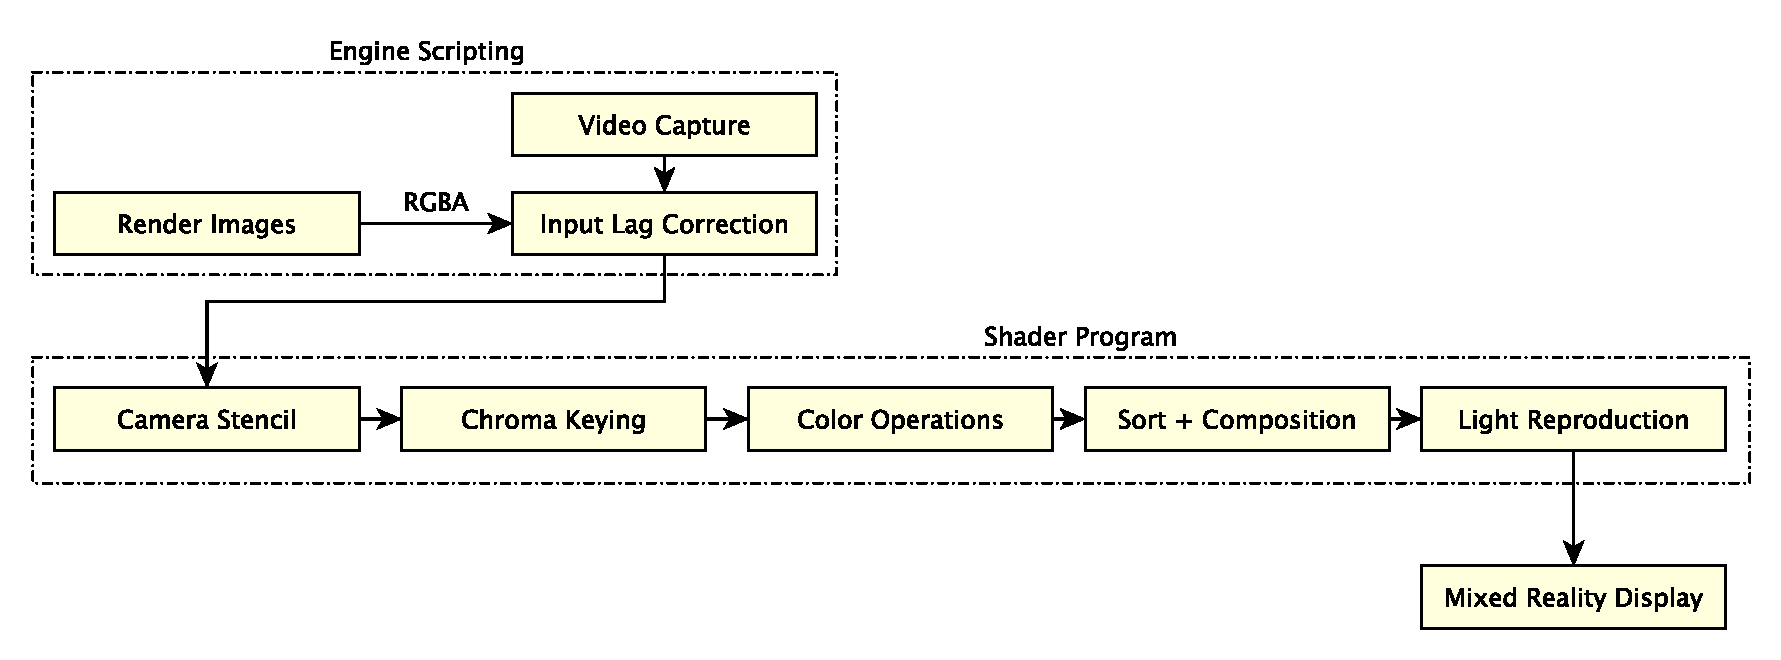
\includegraphics[width=\textwidth]{_raw_resources/pipeline_steps/4_9_order_alt.pdf}
	\caption{Actual order of computation}
	\label{fig:steps:order:alt}
\end{figure}

\todo[inline]{This might be appendix-worthy - then move a note to the chapters' 
beginning.}			  % order of calculation
% !TeX spellcheck = en_US
% !TEX root = ../thesis-example.tex
%
\chapter{Evaluation \& future work}

\section{Hardware setup variations}

Due to the nature of this setup and fine-tweaking options inside the engine, 
this approach discussed can have a wide variety of operational setups. By lose 
coupling of these hardware factors there are only a few limitations that can 
either solved by better, future hardware or a different approach that are 
outside of the scope.

As integral part of this setup is the motion tracking solution, it is possible 
to hook up an Oculus Rift\footnote{with its room-scale setup} instead of the 
HTC Vive and set one controller as camera-attachment point. For that there 
would be another 3D print needed to attach the controller to a camera solution. 
\newline
Other third market VR-HMDs usually follow the Vives specifications closely and 
integrate natively with SteamVR, thus no modification on the original 
instalment has to be done.
\newline
Through Virtual Reality Peripheral Network or OpenVR simliar solutions can be 
developed, since none of the software explicitly depends on SteamVR features 
and allow a wide variety of systems and sensors.

On other side, the video capture side, can be varied greatly too. Since the 
software only allows a webcam-compatible device, it would be possible to remove 
the Inogeni-Encoder and replace it with cheap and simple webcams. Similarly can 
a camera replaced along with other recording solutions, as long as it outputs 
an HDMI (or HDMI-convertible) video stream. This allows recording to be as 
complex as needed but in general a DSLR camera will suffice.

Finally, since the full pipeline is rather complex, a good desktop PC will be 
needed. The CPU overhead is minimal but the graphical complexity is based on 
limitations of the GPU. With future iteration of this hardware it will be 
possible to create more complex scenery, output higher resolution video and 
better frame rates if the video capture device allows for it.
\newline
In theory a low-poly environment could be render-able on mobile, combined with 
a low-sample rate on the camera image, to produce a "window" into VR for 
multiple users at the same time, thus enabling an indefinite view into virtual 
reality. This would remove the MR-pipeline from an actors system. Further work 
could tap into a Microsoft HoloLens solution, which could enable a direct 
contextualization of an actor into a VR scenery without a green screen at all. 
With fast approximate algorithms, like YCgCo-Keying, this could produce a 
high-framerate transparent overlay, so that the virtual scene does not clip the 
actor.

While working with this setup another possible use-case showed up: On June 2017 
Apple presented their native Augmented Reality kit integrated in their consumer 
devices. Thus a similar system could be used to send all tracking parameters 
from the HTC Vive headset to these devices and have a calibrated north-wall 
with additional feature markers. This would potentially allow to have an 
augmented reality view around the actors world with a fast approximated actor 
position. It could then be possible for multiple users to use these devices as 
window into the virtual reality experience without a green screen at all.

\section{Rendering Setup Variations}

There are a few approaches that work similarly, but are different in 
complexity, their capabilities and hardware requirements. They have been 
already explored by producing companies and are covered here for completeness.

\subsection{Single Camera - 3D plane in space}

A novel approach is rendering the camera image onto a 2D plane positioned 
inside the 3D scene. This gives high control over projection parameters inside 
the engine without a running software and has good visual feedback for artists. 
All additional steps previously discussed are invalid, since this render can 
take full advantage of all runtime rendering parameters - which in turn means 
for lower render overhead and better graphical performance. It fails however on 
delay mitigation, which makes time drift between engine and camera visible, 
thus only usable with low latency video capturing devices. (Figure 
\ref{fig:alt-render:single-camera} for reference)

\begin{figure}[htb]
	
\includegraphics[width=\textwidth]{_raw_resources/editor_single_camera.png}
	\caption{Demonstrative scene with a plane as camera rendering position}
	\label{fig:alt-render:single-camera}
\end{figure}

\subsection{Deferred shading Path}

Similarly to the single camera approach could be a deferred shader be used, in 
which the plane is projected and texturized after the scene has rendered and 
the graphics buffer is still present - this way the total time taken for 
rendering can be calculated and the chroma keying step can be chosen for a 
faster variant if needed. This gives generally better control and could yield 
higher performance, since all projected fragments have an assigned depth - the 
camera image only has to be calculated where the actors depth is smaller as the 
sceneries depth. This method is also lacking a way of adjusting for time drift. 
Additionally calculating lightning is relatively expensive, due to the 
reprojection of lighting parameters inside the graphics buffer. A snapshot of 
this buffer cannot be stored - which is a limitation of Unitys render pipeline 
- and is lost after the rendering loop completed.

\subsection{Composition Workstation (4 patch)}

Lastly, for full video production setups another rendering approach has been 
suggested, which was used for the initial promo material 
\cite{valve:vive-trailer:2016} includes rendering a 4K video signal, outputting 
it to a composition PC which then takes care about managing time drift and 
video input from the camera.
\newline
The general concept involves a production of four 1920x1080 video signals of 
the virtual environment:
\begin{my_list}
	\item Foreground
	\item Video matte of foreground
	\item Background
	\item First person view
\end{my_list}

\begin{figure}[htb]
	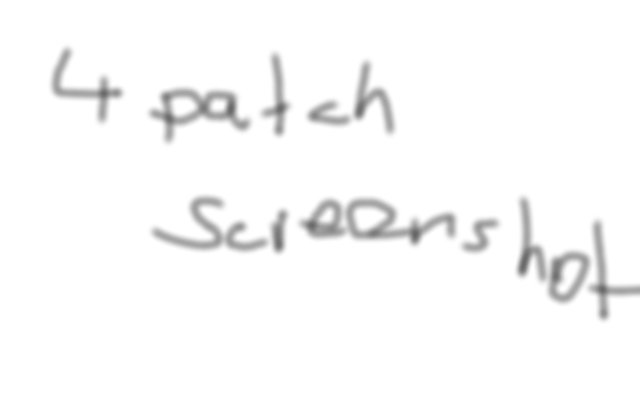
\includegraphics[width=\textwidth]{_raw_resources/4patch_composite.png}
	\caption{Actual order of computation}
	\label{fig:alt-render:4patch}
\end{figure}

Due to the system separation it is now possible to use green screen hardware 
compositor which have a visually higher quality in pulling the green background 
matte and then compositing it similarly into a mixed reality image. While this 
lifts some rendering overhead from the host PC, it fails in recreating a 
lightning environment for the VR actor and relies on two systems. While engine 
programming complexity decreases, operational setup complexity increases.

\section{Rendering operational variations}

This setup can handle another operational context by leaving out 
background-sorting and only rendering a virtual "front", by which a high 
quality augmented camera system can be achieved. Since time drift between 
camera and engine is already handled, it is possible to render an augmented 
image. Since depth information is lost, it is not possible to handle 
obstructions - in example by an interacting user that is standing in front of 
the augmented object. However, with some composition and choreography, AR 
footage can be showed and captured in live production for further use. A 
reference plane has to be used, either by a Vive Tracker\footnote{like a 
controller} or with feature markers.
\newline
This thesis assumes that the motion video feed is calibrated for a D65 white 
and augmented reality scenarios usually do not take real world lightning into 
account, it would give a good natural and high quality look into augmented 
reality use cases.

\section{Edge Cases}

The proposed method has edge cases which could be further improved by other 
approaches in rendering or capturing actor video. These highlight issues 
observed with the rendering operations discussed in this thesis.

\subsection{Image Clipping - incorrect Z calculation for hands}

Due to the planar projection of the real world feed inside the engine, any 
Z-information of the actor is squashed to a fixed depth. This means that hands 
are on the same plane. In cases with high z-difference between actor and actors 
hands, it is possible that hand motion look unnatural and does not seems like 
it is to be supposed - in figure \ref{fig:edge:z-clipping} is an actor 
depicted, that wraps his arms around a virtual cube. The produced mixed reality 
image shows his arms only behind the cube.

\begin{figure}[htb]
	\centering
	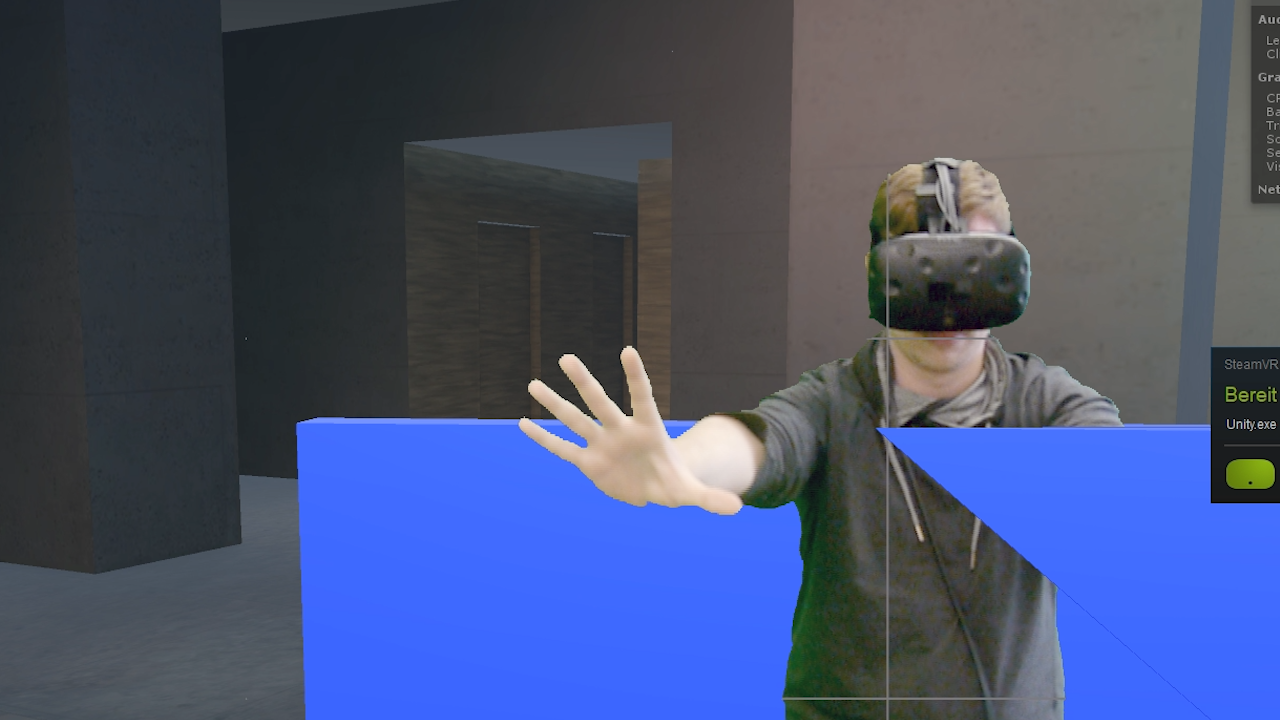
\includegraphics[width=\textwidth]{gfx/issues/z-clipping.png}
	\caption{The actors hands do not visibly reach through the blue cube and 
	the actor shears it because of the planar projection}
	\label{fig:edge:z-clipping}
\end{figure}

One solution for future research could be acquiring an actors depth by either 
using Time of Flight cameras and using a resulting point cloud or by 
calculating each camera pixels depth with a stereoscopic solution. Thus each 
pixel could have a quantifiable depth with additional calibration parameters 
from the virtual reality tracking solution.

\subsection{Matting failures}

There are multiple problems while green screening, which are as old as green 
screens are used in video production. First and foremost is a partial 
transparent actor if his clothing consists of similarly green shaded material.
\newline
Additional green screen spill causes artefacts while pulling the matte which 
then clips the actor off. This can be mitigated by better production 
environments, i. e. with higher quality cloth and a generally well lit set. 
\footnote{The appendix features a basic schematic of a small green screen 
setup.}
\newline
Sometimes, for example in low light environments or folded green screen 
material, the background covers a wide color range, thus calibrating a good 
green with a single color value is nearly impossible. This could be solved by 
smaller selection margins inside the shader while assigning an array of colors 
for the $\Delta E$ calculation. In turn, this would be even more taxing on the 
GPU, since the calculation has be done per selected color.
\newline
Lastly, real time chroma keying has problems with motion blur of the source 
video material - causing background mixing and invalid matting. This is a 
complex problem that is far beyond the scope of this thesis. One of the best 
solutions is a color unmixing approach researched by Disney and "typically 
requires 10s for local color estimation (assuming 8 dominant colors), another 
second to propagate the local color model to the following frame, and 
approximately 3s for color unmixing." \cite{disney:unmixing:2017}
\todo{Add graphics depicting each issue. Also cross reference to chapter 4}

\subsection{Calibration problems (wrong clipping, wrong reprojection, long 
setup times)}

The biggest margin of error is calibration of all projection parameters.
\newline
Beginning from field of view calculation, most DSLR cameras don't have 
specifications for their output feeds, where, for example, scaling factors 
could change the field of view angle. If these are not given or seem to be 
unfitting in production it is necessary to measure these parameters by hand, 
fixing the cameras position and calculating the spanning angle.
\todo{maybe add the ez calculation, too}
Another factor are offset-parameters between controllers and camera sensor, 
which have been minimized by the 3D printed attachment. However, minimal 
differences in this transformation matrix have tremendous impact on 
miscalculated projections, visible by wrongly placed objects and a disconnect 
between virtual interaction and actor.
\todo{Here comes a graphical representation of it}
Lastly, the most time spent after adding all mixed reality components to the 
scene is calibrating these parameters. A possible improvement could be done by 
fixing the cameras position, showing an overlay on the camera, where the 
secondary controller has to be placed and confirming it. This way the user can 
calibrate all projection parameters by himself with the help of a RANSAC / 
Lagrange Polynomial.
\todo[inline]{find out how this calibration is called: 
https://www.youtube.com/watch?v=c\_An0vxvPnk}
% !TEX root = ../thesis-example.tex
%
\chapter{Conclusion}

\subsection{3D Environment and Composition Considerations}
\subsection{Performance Considerations}
% !TEX root = ../thesis-example.tex
%
% \chapter{Related Work}
% 
% \section{Green Screen Video Composition}
% \section{Video Matting}
% \section{PostFX Mixed Reality}
% \section{Realtime Mixed Reality}
% % !TEX root = ../thesis-example.tex
%
\chapter{Concepts: This text is here to test a very long title, to simulate the line break behavior, to show that an extremely long tilte also works}
\label{sec:concepts}

\cleanchapterquote{Users do not care about what is inside the box, as long as the box does what they need done.}{Jef Raskin}{about Human Computer Interfaces}

\Blindtext[2][1]

\section{Concepts Section 1}
\label{sec:concepts:sec1}

\Blindtext[2][2]

\section{Concepts Section 2}
\label{sec:concepts:sec2}

\Blindtext[3][2]

\section{Concepts Section 3}
\label{sec:concepts:sec3}

\Blindtext[4][2]

\section{Conclusion}
\label{sec:concepts:conclusion}

\Blindtext[2][1]
 % INCLUDE: concepts
% % !TEX root = ../thesis-example.tex
%
\chapter{Conclusion}

\subsection{3D Environment and Composition Considerations}
\subsection{Performance Considerations} % INCLUDE: conclusion
\cleardoublepage

\begin{appendices}
	\printglossary
	\cleardoublepage
	% !TeX spellcheck = en_US
% !TEX root = ../thesis-example.tex
%

\chapter{Unitys' Monobehaviour Loop}
\label{app:engineloop}

The behavior of a Unity-initiated object is outlined by the following 
flowchart in \ref{fig:appendix:flowchart}, taken from Unitys' manual.

\begin{figure}[htb]
	\centering
	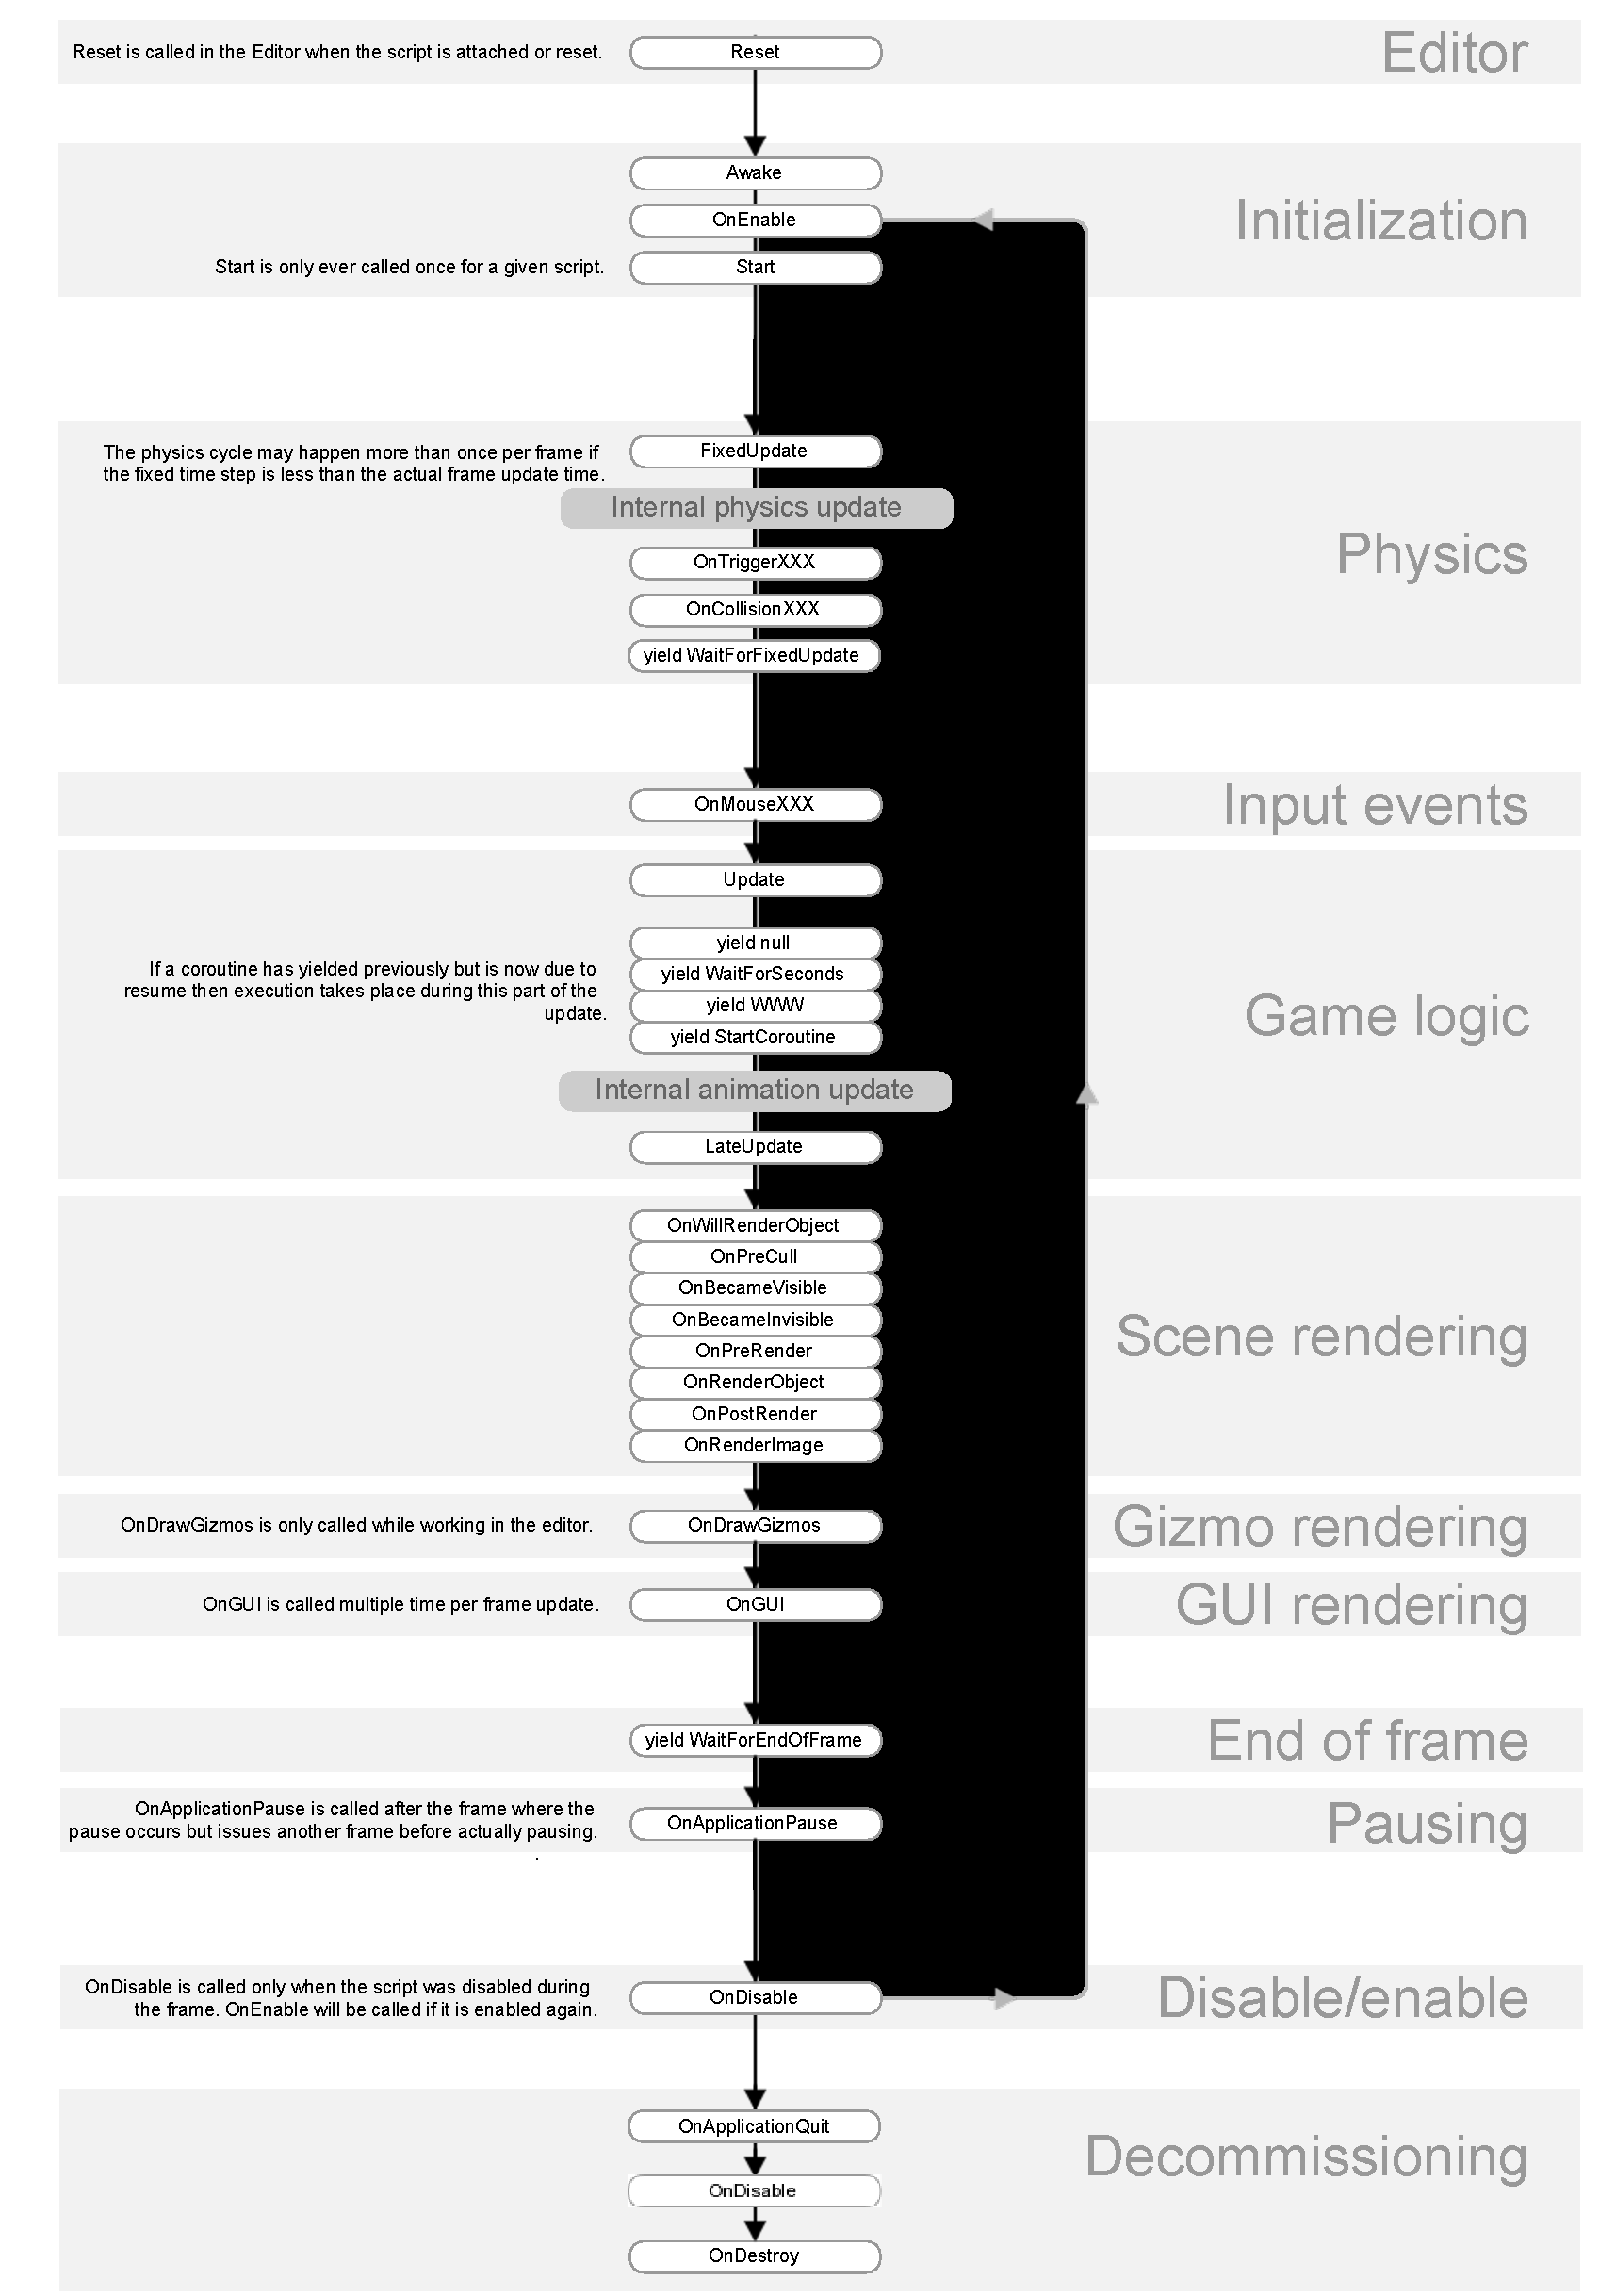
\includegraphics[width=0.85\textwidth]{_external/media/monobehaviour_flowchart.pdf}
	\caption{Monobehaviour Flowchart}
	\label{fig:offsets:components}
\end{figure}
\end{appendices}


% --------------------------
% Back matter
% --------------------------
{%
\setstretch{1.1}
\renewcommand{\bibfont}{\normalfont\small}
\setlength{\biblabelsep}{0pt}
\setlength{\bibitemsep}{0.5\baselineskip plus 0.5\baselineskip}
\printbibliography[nottype=online]
\printbibliography[heading=subbibliography,title={Websites},type=online]
}
\cleardoublepage

\listoffigures
\cleardoublepage

\listoftables
\cleardoublepage

% !TEX root = ../thesis-example.tex
%
\pagestyle{empty}
\hfill
\vfill
\pdfbookmark[0]{Colophon}{Colophon}
\section*{Colophon}

This thesis was typeset with \LaTeXe.
It uses the \textit{Clean Thesis} style developed by Ricardo Langner.
The design of the \textit{Clean Thesis} style is inspired by user guide documents from Apple Inc.

Download the \textit{Clean Thesis} style at \url{http://cleanthesis.der-ric.de/}.

\cleardoublepage

% !TEX root = ../thesis-example.tex
%
%************************************************
% Declaration
%************************************************
\pdfbookmark[0]{Declaration}{Declaration}
\chapter*{Declaration}
\label{sec:declaration}
\thispagestyle{empty}

Hereby I affirm that this thesis is written by myself and I have not used any 
additional resources or utilities.

\begin{center}
	\hrulefill
\end{center}

Ich versichere, dass ich meine Abschlussarbeit selbstständig verfasst und keine 
anderen als die angegebenen Quellen und Hilfsmittel benutzt habe.

\bigskip

\noindent\textit{\thesisUniversityCity, \thesisDate}

\smallskip

\begin{flushright}
	\begin{minipage}{5cm}
		\rule{\textwidth}{1pt}
		\centering\thesisName, Matr.-Nr. 824320
	\end{minipage}
\end{flushright}

%*****************************************
%*****************************************

\clearpage
\newpage
\mbox{}

% **************************************************
% End of Document CONTENT
% **************************************************
\end{document}
